%%%%%%%%%%%%%%%%%%%%%%%%%%%%%%%%%%%%%%%%%
% Diploma Thesis
% Dimitrios Tikvinas
% November 2024
%%%%%%%%%%%%%%%%%%%%%%%%%%%%%%%%%%%%%%%%%

%----------------------------------------------------------------------------------------
%	PACKAGES AND OTHER DOCUMENT CONFIGURATIONS
%----------------------------------------------------------------------------------------

\documentclass[
12pt, % The default document font size, options: 10pt, 11pt, 12pt
twoside, % Two side (alternating margins) for binding by default, uncomment to switch to one side
openright,
%chapterinoneline,% Have the chapter title next to the number in one single line
english,
%singlespacing, % Single line spacing, alternatives: onehalfspacing or doublespacing
%draft, % Uncomment to enable draft mode (no pictures, no links, overfull hboxes indicated)
%nolistspacing, % If the document is onehalfspacing or doublespacing, uncomment this to set spacing in lists to single
%liststotoc, % Uncomment to add the list of figures/tables/etc to the table of contents
%toctotoc, % Uncomment to add the main table of contents to the table of contents
%parskip, % Uncomment to add space between paragraphs
%nohyperref, % Uncomment to not load the hyperref package
headsepline, % Uncomment to get a line under the header
]{MastersDoctoralThesis} % The class file specifying the document structure

\usepackage{xltxtra}
\usepackage{xgreek}
\setmainfont[Mapping=tex-text]{GFS Didot}
\usepackage{amsfonts}
\usepackage[Greek,Latin]{ucharclasses}
\setTransitionsForGreek{\setlanguage{greek}}{\setlanguage{american}}
\setmainfont[Kerning=On,Mapping=tex-text]{Linux Libertine O}

\usepackage[backend=biber, sorting=none, maxcitenames=2]{biblatex}


\usepackage[autostyle=true]{csquotes} % Required to generate language-dependent quotes in the bibliography

\usepackage{subfig}

\usepackage{datetime}
\newdateformat{monthyeardate}{%
  \monthname[\THEMONTH] \THEYEAR}

\def\monthyeargreek{%
  \def\today{\ifcase\month\or
      Ιανουάριος\or Φεβρουάριος\or Μάρτιος\or Απρίλιος\or Μάιος\or Ιούνιος\or
      Ιούλιος\or Αύγουστος\or Σεπτέμβριος\or Οκτώβριος\or Νοέμβριος\or
      Δεκέμβριος\fi\space
      \number\year}%
}


\usepackage{amsmath}
\usepackage{amssymb}
%\usepackage{algorithmicx}
\usepackage{algpseudocode}
\usepackage{algorithm}
\algdef{SE}[DOWHILE]{Do}{doWhile}{\algorithmicdo}[1]{\algorithmicwhile\ #1}%

\usepackage{url}

\usepackage{placeins}

\usepackage{multirow}
\usepackage[table,xcdraw]{xcolor}

% Language transitions
\usepackage[Greek,Latin]{ucharclasses}
\setTransitionsForGreek{\setlanguage{greek}}{\setlanguage{english}}

\usepackage{float}

% Theorem environments
\usepackage{amsthm}

% Underlining package (using 'ulem' for better compatibility)
\usepackage[normalem]{ulem} % Provides the \uline{} command for underlining

% Hyperlinks and intelligent referencing
\usepackage{hyperref}
\usepackage{cleveref}

\NewDocumentCommand{\bref}{O{blue}mo}{%
  \begingroup
  \hypersetup{linkbordercolor=#1}%
  \ref{#2}%
  \IfValueT{#3}{%
    \color{#1}{#3}%
  }%
  \endgroup
}% %NEW COMMAND ALTERNATIVE TO REF

% Make \uline robust to prevent errors in moving arguments
\DeclareRobustCommand{\ulinecmd}[1]{\uline{#1}}


% Define a custom theorem style with underlined headers
\newtheoremstyle{underline} % Name of the style
  {3pt}                     % Space above
  {3pt}                     % Space below
  {\itshape}                % Body font
  {}                        % Indent amount
  {}                        % Theorem head font (will be defined in head spec)
  {.}                       % Punctuation after theorem head
  { }                       % Space after theorem head
  {\bfseries\ulinecmd{#1~#2}} % Theorem head spec: bold and underlined title and number

% Apply the custom theorem style
\theoremstyle{underline}
\newtheorem{observation}{Παρατήρηση}[chapter]
\newtheorem{hypothesis}{Υπόθεση}[chapter]
\newtheorem{conclusion}{Συμπέρασμα}[chapter]
\newtheorem{theorem}{Θεώρημα}[chapter]
\newtheorem{proof_of_theorem}{Απόδειξη Θεωρήματος}[chapter]
\newtheorem{step}{Βήμα}[section]
\newtheorem{definition}{Ορισμός}[chapter]


% Configure cleveref for the new environments
\crefname{observation}{Παρατήρηση}{Παρατηρήσεις}
\Crefname{observation}{Παρατήρηση}{Παρατηρήσεις}

\crefname{hypothesis}{Υπόθεση}{Υποθέσεις}
\Crefname{hypothesis}{Υπόθεση}{Υποθέσεις}

\crefname{conclusion}{Συμπέρασμα}{Συμπεράσματα}
\Crefname{conclusion}{Συμπέρασμα}{Συμπεράσματα}

\crefname{theorem}{Θεώρημα}{Θεωρήματα}
\Crefname{theorem}{Θεώρημα}{Θεωρήματα}

\crefname{proof_of_theorem}{Απόδειξη Θεωρήματος}{Αποδείξεις Θεωρημάτων}
\Crefname{proof_of_theorem}{Απόδειξη Θεωρήματος}{Αποδείξεις Θεωρημάτων}

\crefname{definition}{Ορισμός}{Ορισμοί}
\Crefname{definition}{Ορισμός}{Ορισμοί}





\captionsetup[table]{name=Πίνακας}

\renewcommand*\descriptionlabel[1]{\hspace\leftmargin$#1$}

\addbibresource{references.bib} % The filename of the bibliography

%----------------------------------------------------------------------------------------
%	MARGIN SETTINGS
%----------------------------------------------------------------------------------------

\geometry{
	paper=a4paper, % Change to letterpaper for US letter
	inner=2.5cm, % Inner margin
	outer=2.5cm, % Outer margin
	bindingoffset=0cm, % Binding offset
	top=1.5cm, % Top margin
	bottom=1.5cm, % Bottom margin
	%showframe %show how the type block is set on the page
}

%----------------------------------------------------------------------------------------
%	THESIS INFORMATION
%----------------------------------------------------------------------------------------
\thesistitle{Έλεγχος διμερούς ρομποτικού τηλεχειρισμού με άγνωστες χρονικές καθυστερήσεις και εγγυήσεις απόδοσης και ασφάλειας}
\thesisengtitle{}
\supervisor{Γεώργιος Ροβιθάκης \\Καθηγητής Α.Π.Θ.}
\degree{Δίπλωμα Ηλεκτρολόγου Μηχανικού και Μηχανικού Ηλεκτρονικών Υπολογιστών}
\author{Τικβίνας Δημήτριος}

\university{ΑΡΙΣΤΟΤΕΛΕΙΟ ΠΑΝΕΠΙΣΤΗΜΙΟ ΘΕΣΣΑΛΟΝΙΚΗΣ}
\department{Τμήμα Ηλεκτρολόγων Μηχανικών και Μηχανικών Υπολογιστών}
\group{Τομέας Ηλεκτρονικής και Υπολογιστών}
\faculty{ΠΟΛΥΤΕΧΝΙΚΗ ΣΧΟΛΗ}

\subject{}
\keywords{}

\hypersetup{pdftitle=\ttitle}
\hypersetup{pdfauthor=\authorname}
\hypersetup{pdfkeywords=\keywordnames}

\begin{document}

\frontmatter % Use roman page numbering style (i, ii, iii, iv...) for the pre-content pages
\pagestyle{plain}

%----------------------------------------------------------------------------------------
%	TITLE PAGE
%----------------------------------------------------------------------------------------

\begin{titlepage}
	\begin{center}

		% University/department logo - uncomment to place it
		\input{Figures/auth_logo.pdf_tex}\\[0.2cm]

		% university name
		{\large \univname}\\[0.2cm]
		% faculty name
		{\large \facname}\\[0.2cm]
		% department name
		\deptname\\
		% group of department name
		\groupname\\[2.5cm]  % Reduced space from 3cm to 2.5cm

		{\LARGE Διπλωματική Εργασία}\\[0.8cm] % Reduced space from 1cm to 0.8cm

		\HRule \\[0.3cm] % Reduced space from 0.4cm to 0.3cm
		{\huge \bfseries \ttitle\par}\vspace{0.3cm} % Reduced space from 0.4cm to 0.3cm
		\HRule \\[2.5cm] % Reduced space from 3cm to 2.5cm

		\begin{minipage}[t]{0.45\textwidth}  % Widened the minipage to 0.45 to avoid too much vertical space
			\begin{flushleft} \large
				\emph{\textbf{Εκπόνηση:}}\\ \authorname
			\end{flushleft}
		\end{minipage}
		\begin{minipage}[t]{0.45\textwidth}  % Widened the minipage to 0.45 to avoid too much vertical space
			\begin{flushright} \large
				\emph{\textbf{Επιβλέπων:}} \\
				\supname % Supervisor name - remove the \href bracket to remove the link
			\end{flushright}
		\end{minipage}\\[2.5cm] % Reduced space from 3cm to 2.5cm

		\vfill
		{\large Θεσσαλονίκη, \monthyeargreek\today} % Date
	\end{center}
\end{titlepage}


%\let\cleardoublepage\clearpage % comment out to add empty empty pages for printed version

\mbox{}
\thispagestyle{empty}
\newpage

%----------------------------------------------------------------------------------------
%	SUMMARY PAGE
%----------------------------------------------------------------------------------------

\begin{summary}
	%\addchaptertocentry{\summaryname} % Add the summary to the table of contents
	Σύγχρονα συστήματα διμερούς τηλεχειρισμού ρομποτικών μονάδων ηγέτη-Ακόλουθου, τα οποία έχουν αναδειχθεί ως χρήσιμο εργαλείο σε πολλούς τομείς, παρουσιάζουν σημαντικές προκλήσεις κυρίως όσον αφορά την αξιόπιστη και ακριβή απόδοση παρακολούθησης και την ικανοποίηση περιορισμών κατάστασης για την επίτευξη των απαιτούμενων προδιαγραφών ασφάλειας. Ωστόσο, αυτές οι προκλήσεις μπορεί να είναι αντιφατικές, καθιστώντας απαραίτητη την εισαγωγή ενός ισορροπημένου συμβιβασμού μέσω του σχεδιασμού ελέγχου. Από τη μια πλευρά, ο στόχος ελέγχου του Ακόλουθου είναι να παρακολουθεί με υψηλή ακρίβεια και αυξημένη ανταπόκριση την τροχιά του ηγέτη, η οποία καθοδηγείται από την ανθρώπινη δράση, ενώ και τα δύο ρομποτικά συστήματα πρέπει να ικανοποιούν ορισμένους περιορισμούς κατάστασης για να διασφαλίσουν τις απαιτούμενες προδιαγραφές ασφάλειας. Είναι προφανές ότι η απρόβλεπτη ανθρώπινη δράση μπορεί να οδηγήσει την τροχιά του ηγέτη σε περιοχές όπου η ασφάλεια και των δύο συστημάτων βρίσκεται σε υψηλό κίνδυνο. Αυτό καθιστά απαραίτητη τη δυναμική μεταβολή των προτεραιοτήτων ελέγχου, όποτε είναι αναγκαίο, δίνοντας έμφαση σε δείκτες ασφάλειας εις βάρος της ακριβούς παρακολούθησης του ηγέτη. Η προτεινόμενη αρχιτεκτονική ελέγχου βασίζεται σε έναν σχεδιασμό ελέγχου ανατροφοδότησης κατάστασης χαμηλής πολυπλοκότητας, αξιοποιώντας τη μεθοδολογία ελέγχου προκαθορισμένης απόδοσης (PPC), η οποία, με τις κατάλληλες τροποποιήσεις, είναι ικανή να αντιμετωπίσει αυτό το ανταγωνιστικό δίλημμα. Ο προτεινόμενος σχεδιασμός ελέγχου είναι ανθεκτικός σε αβέβαιες καθυστερήσεις επικοινωνίας και, εκτός από την εγγύηση ότι όλα τα σήματα στο κλειστό κύκλωμα παραμένουν εντός ορίων, διασφαλίζει επίσης ότι η εξέλιξη του σφάλματος παρακολούθησης ηγέτη-Ακόλουθου περιορίζεται αυστηρά εντός προκαθορισμένων ορίων, ενώ ταυτόχρονα επιβάλλει περιορισμούς κατάστασης σχετικούς με την ασφάλεια, σε περίπτωση που η τροχιά του ηγέτη θέτει σε κίνδυνο την ασφάλεια των δύο ρομποτικών συστημάτων. Τα θεωρητικά αποτελέσματα επαληθεύονται και διευκρινίζονται μέσω προσομοιώσεων.
	
	
	
	
	\bigskip
	\end{summary}
	
	
	%----------------------------------------------------------------------------------------
	%	ABSTRACT PAGE
	%----------------------------------------------------------------------------------------
	
	\begin{abstract}
	%\addchaptertocentry{\abstractname} % Add the abstract to the table of contents
	Modern leader-follower robotic teleoperation systems that have emerged as a useful tool in many fields, demonstrate significant challenges mainly concerning the reliable and accurate tracking performance and the satisfaction of state constraints to meet the required safety specifications. However, these challenges may be conflicting, making it necessary to introduce, via the control design, a balanced compromise. On one hand, the control objective of the follower is to track the trajectory of the leader, which is driven by the human action, with high precision and increased responsiveness, while both robotic systems should satisfy certain state constraints to guarantee the required safety specifications. Apparently, the unpredictable human action may force the leader-trajectory to regions where the safety of both systems is at high risk. This necessitates a dynamic shift in control priorities, whenever necessary, by placing emphasis on safety indices at the expense of accurate leader tracking performance. The proposed control architecture is based on a low-complexity state-feedback control design, leveraging the methodology of prescribed performance control (PPC), which, with proper modifications, is capable of addressing this competing dilemma. The proposed control design is robust with respect to uncertain communication delays, and besides the boundedness of all signals in the closed-loop, it further guarantees that the evolution of the leader-follower tracking error is confined strictly within pre-defined bounds, while simultaneously enforces safety-related state constraints, in case the leader-trajectory jeopardizes the safety of the two robotic systems. The theoretical results are verified and clarified through simulation studies.
	\bigskip
	
	\begin{flushright}
	{\normalsize Tikvinas Dimitrios \par} % Author name
	{\normalsize Electrical and Computer Engineering Department \par} % Department name
	{\normalsize Aristotle University of Thessaloniki, Greece \par} % University name in capitals
	{\normalsize \monthyeardate\today}
	\end{flushright}
	
	\end{abstract}
	
	%----------------------------------------------------------------------------------------
	%	ACKNOWLEDGEMENTS
	%----------------------------------------------------------------------------------------
	
	\begin{acknowledgements}
	%\addchaptertocentry{\acknowledgementname} % Add the acknowledgements to the table of contents
	Αρχικά, θα ήθελα να ευχαριστήσω τον επιβλέποντα καθηγητή μου, κ. Γεώργιο Ροβιθάκη, για την εμπιστοσύνη που έδειξε στο πρόσωπο μου ϰαι την επιστημονιϰή ϰαϑοδήγησή του ϰαϑόλη τη διάρϰεια εϰπόνησης της παρούσας διπλωματιϰής εργασίας.

	\bigskip
	Επιπλέον, θα ήθελα να εκφράσω τις θερμές μου ευχαριστίες στον μεταδιδακτορικό ερευνητή Λάμπρο Μπίκα για την συνεχή, άμεση υποστήριξη και τις συμβουλές του πάνω στο θέμα, τον πολύτιμο χρόνο που με διέθεσε και γενιϰότερα την άψογη συνεργασία που είχαμε στα πλαίσια διεϰπεραίωσης αυτής της εργασίας.

	\bigskip
	Τέλος, ένα μεγάλο ευχαριστώ χρωστάω τους γονείς μου που κάθε στιγμή ήταν εκεί και τους στενούς μου ανθρώπους για την συνολιϰή ενϑάρρυνση, στήριξη και ανοχή που εϰφράζουν όλα αυτά τα χρόνια των σπουδών μου.
	
	\end{acknowledgements}

	\let\cleardoublepage\clearpage
	
	%----------------------------------------------------------------------------------------
	%	LIST OF CONTENTS/FIGURES/TABLES PAGES
	%----------------------------------------------------------------------------------------
	
	\renewcommand{\contentsname}{Πίνακας Περιεχομένων}
	\tableofcontents % Prints the main table of contents
	\let\cleardoublepage\clearpage
	
	\renewcommand{\listfigurename}{Λίστα Σχημάτων}
	\listoffigures % Prints the list of figures
	\renewcommand{\figurename}{Σχήμα}
	\let\cleardoublepage\clearpage
	
	%----------------------------------------------------------------------------------------
	%	ABBREVIATIONS
	%----------------------------------------------------------------------------------------
	
	\begin{abbreviations}{ll} % Include a list of abbreviations (a table of two columns)
	%
	\textbf{ΣΔΤΗΑ} & \textbf{Σ}υστήματα \textbf{Δ}ιμερούς \textbf{Τ}ηλεχειρισμού \textbf{Η}γέτη \textbf{Α}κόλουθου\\
	\textbf{ΕΠΑ} & \textbf{Έ}λεγχος \textbf{Π}ροδιαγεγραμμένης \textbf{Α}πόκρισης\\
	\textbf{ΠΑΑ} & \textbf{Π}εριοχή \textbf{Α}σφαλείας \textbf{Α}κόλουθου\\
	\textbf{ΠΚΑ} & \textbf{Π}εριοχή \textbf{Κ}ινδύνου \textbf{Α}κόλουθου\\
	\end{abbreviations}

	\let\cleardoublepage\clearpage
	
	%----------------------------------------------------------------------------------------
	%	SYMBOLS
	%----------------------------------------------------------------------------------------
	
	%\begin{symbols}{lll} % Include a list of Symbols (a three column table)
	%
	%$a$ & distance & \si{\meter} \\
	%$P$ & power & \si{\watt} (\si{\joule\per\second}) \\
	%%Symbol & Name & Unit \\
	%
	%\addlinespace % Gap to separate the Roman symbols from the Greek
	%
	%$\omega$ & angular frequency & \si{\radian} \\
	%
	%\end{symbols}
	
	%----------------------------------------------------------------------------------------
	%	THESIS CONTENT - CHAPTERS
	%----------------------------------------------------------------------------------------
	
	\mainmatter % Begin numeric (1,2,3...) page numbering
	
	\pagestyle{thesis} % Return the page headers back to the "thesis" style
	
	% change chapter label
	\renewcommand{\chaptername}{Κεφάλαιο}
	
	% include chapters
	\chapter{Εισαγωγή} \label{Chapter1}


%----------------------------------------------------------------------------------------
%	SECTION 1
%----------------------------------------------------------------------------------------

\section{Συστήματα Διμερούς Τηλεχειρισμού} \label{Chapter1Section1}
Τα \textbf{Συστήματα Διμερούς Τηλεχειρισμού Ηγέτη-Ακόλουθου - ΣΔΤΗΑ} (Leader-Follower teleoperation systems) είναι συστήματα κλειστού βρόχου που αποτελούνται από δύο ρομποτικούς βραχίονες: τον ηγέτη (Leader), ο οποίος χειρίζεται από έναν άνθρωπο, και τον ακολούθο (Follower), ο οποίος έχει ως κύριο στόχο να ακολουθεί και να αναπαράγει με ακρίβεια την τροχιά του πρώτου. Η γενική τους μορφή παρουσιάζεται στο Σχήμα (\bref{generic_implementation}).

\bigskip
Με τη ραγδαία ανάπτυξη που έχει σημειωθεί στον χώρο της ρομποτικής, τα συστήματα αυτά έχουν αποκτήσει ιδιαίτερη σημασία, καθώς προσφέρουν τη δυνατότητα εκτέλεσης σύνθετων και επικίνδυνων εργασιών σε απομακρυσμένα ή δυσπρόσιτα περιβάλλοντα, συνδυάζοντας την ανθρώπινη εμπειρία και κρίση με την ακρίβεια και την αντοχή των ρομποτικών συστημάτων, με απότοκο την μεγιστοποίηση της αποδοτικότητας και της ασφάλειας. Επιπλέον, σε τέτοιου είδους πρακτικές εφαρμογές, κρίνεται σημαντική η χρήση διμερούς επικοινωνίας, δηλαδή της παροχής απτικής ανάδρασης στον χειριστή. Αυτή η προσέγγιση τού προσδίδει διαδραστικότητα, με το να αισθάνεται δυνάμεις και αντιστάσεις που αντιμετωπίζει ο Ακόλουθος, βελτιώνοντας έτσι τον έλεγχο . 

\bigskip
Ως απόρροια των παραπάνω, σε συνδυασμό με την ταχεία πρόοδο και χρήση του διαδικτύου, των τεχνολογιών ασύρματης επικοινωνίας και κυρίως των ρομποτικών βραχιόνων, τα ΣΔΤΗΑ ενσωματώνονται σε ένα ευρύ φάσμα εφαρμογών. Συγκεκριμένα, εφαρμόζονται σε αποστολές έρευνας και διάσωσης με τη συγχρονισμένη τηλεχειριστική λειτουργία μεταξύ πολλών ρομποτικών συστημάτων, όπως προτείνουν οι Qureshi \textit{et al.} (2016)\cite{qureshi2016leader}. Επίσης, σε στρατιωτικά συστήματα επιτήρησης μέσω του τηλεχειρισμού στόλου UAV (Unmanned Aerial Vehicles) σε πραγματικό χρόνο, όπως αναφέρουν οι Hunukumbure \textit{et al.} (2013)\cite{hunukumbure2013teleoperation}, και στη ρομποτική χειρουργική, όπου ο χειρουργός-χειριστής ελέγχει το κύριο ρομπότ ενώ ένα ή περισσότερα ακόλουθα ρομπότ συντονίζουν τις ενέργειές τους, σύμφωνα με τους Guo \textit{et al.} (2018)\cite{guo2018leader}. Επιπλέον, τα ΣΔΤΗΑ χρησιμοποιούνται στην τηλεχειριστική λειτουργία αυτόνομων οχημάτων σε δυναμικά περιβάλλοντα, επιτρέποντας τη δημιουργία φάλαγγας οχημάτων υπό απομακρυσμένο έλεγχο, όπως παρουσιάζουν οι Jaloudi και Alloghani (2019)\cite{jaloudi2019leader}. Στον τομέα των υποβρύχιων ερευνών, αυτά τα συστήματα εφαρμόζονται σε επιθεωρήσεις αγωγών και εξερευνήσεις βαθέων υδάτων, όπως περιγράφουν οι Yuan \textit{et al.} (2021)\cite{yuan2021leader}. Στην αγροτική βιομηχανία, τα ΣΔΤΗΑ ενισχύουν την παραγωγικότητα σε εκτεταμένες γεωργικές εκτάσεις, όπου ένας ηγέτης-ρομπότ κατευθύνει πολλαπλές αυτόνομες μηχανές, σύμφωνα με τους Hou \textit{et al.} (2017)\cite{hou2017leader}. Τέλος, στη βιομηχανική παραγωγή, χρησιμοποιούνται για τον συντονισμό εργασιών σε επαναλαμβανόμενες ή επικίνδυνες διαδικασίες, όπως αναφέρουν οι Nakamura \textit{et al.} (2017)\cite{nakamura2017leader}.

\bigskip
Τα τελευταία χρόνια, το πρόβλημα του διμερούς τηλεχειρισμού Ηγέτη-Ακόλουθου με καθυστερήσεις επικοινωνίας έχει προσελκύσει σημαντικό ενδιαφέρον, και έχουν σημειωθεί αξιοσημείωτες πρόοδοι. Συγκεκριμένα, η ασυμπτωτική ευστάθεια του σφάλματος παρακολούθησης εξόδου έχει εδραιωθεί στα έργα των Chopra \textit{et al.} (2008)\cite{chopra2008synchronization}, Mohammadi \textit{et al.} (2012)\cite{mohammadi2012control}, Wang (2021)\cite{wang2021bilateral}, Estrada \textit{et al.} (2021)\cite{estrada2021stable} και Zhang \textit{et al.} (2022)\cite{zhang2022adaptive}. Επιπλέον, η ομοιόμορφη τελική φραγμένη συμπεριφορά έχει μελετηθεί στα έργα των Ohkawa και Yamashita (2011)\cite{ohkawa2011passivity}, Liu και Chopra (2013)\cite{liu2013control} και Abdessameud \textit{et al.} (2017)\cite{abdessameud2017leader}. Τέλος, η παθητικότητα του κλειστού βρόχου συστήματος μαζί με την ασυμπτωτική ευστάθεια του σφάλματος παρακολούθησης ηγέτη-Ακόλουθου έχει αναδειχθεί στα έργα των Forouzantabar \textit{et al.} (2012)\cite{forouzantabar2012bilateral}, Yan \textit{et al.} (2014)\cite{yan2014consensus}, Li και Kawashima (2016)\cite{li2016bilateral}, Nuño \textit{et al.}(2018)\cite{nuno2018control} και Su \textit{et al.}(2020)\cite{su2020bilateral}. Όμως, δεν προσφέρουν κάποια θεωρητική απόδειξη του ακριβές σφάλματος παρακολούθησης	πέρα από την ευστάθεια και την ασυμπτωτική του σύγκλιση, ένα πρόβλημα που επίλυσε το έργο (Bikas, Rovithakis) \textit{et al.}(2023)\cite{BIKAS20239972}. Το έργο αυτό, ακολουθώντας τον Έλεγχο Προδιαγεγραμμένης Απόκρισης (βλέπε \bref{Chapter2Section1}), καθώς και την ΕΠΑ λύση στο πρόβλημα παρακολούθησης μιας φραγμένης τροχιάς αναφοράς παρουσία χρονικών καθυστερήσεων στις καταστάσεις ή/και στην είσοδο ελέγχου (Bikas, Rovithakis) \textit{et al.}(2019) \cite{bikas2019enhancing}, \textit{et al.}(2021) \cite{bikas2021prescribed}, κατάφερε την ζητούμενη αξιόπιστη και προδιαγεγραμμένη παρακολούθηση με συγκεκριμένο ρυθμό σύγκλισης, θεωρώντας γνωστή και σταθερή καθυστέρηση στο κανάλι επικοινωνίας.

\bigskip
\begin{figure}[!ht]
  \begin{center}
    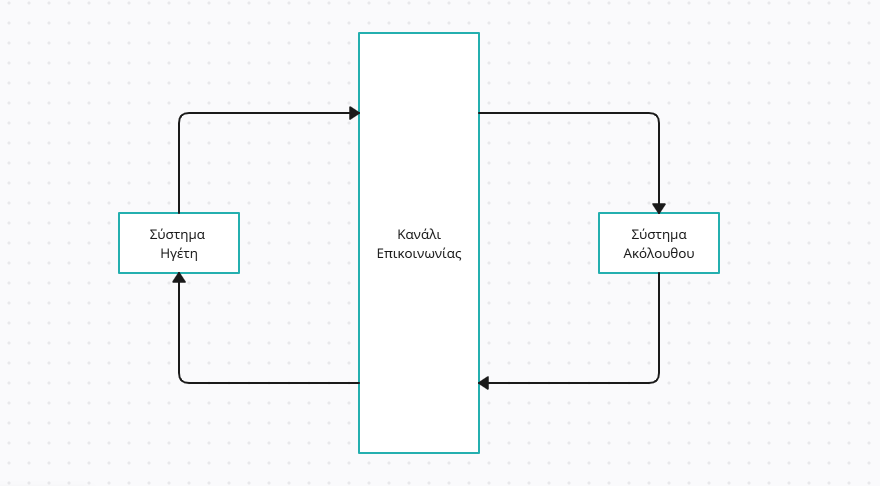
\includegraphics[width=1\linewidth]{Chapters/Chapter1/Figures/Generic_Implementation.png}
    \caption[Γενική Δομή των ΣΔΤΗΑ]{Γενική Δομή των ΣΔΤΗΑ}
    \label{generic_implementation}
  \end{center}
\end{figure}

\bigskip
Ένα σημαντικό ζήτημα που ανακύπτει είναι ότι οι καθυστερήσεις στο ψηφιακό κανάλι επικοινωνίας παραμένουν, στις περισσότερες περιπτώσεις, απρόβλεπτες και μη σταθερές, γεγονός που καθιστά τον έλεγχο σχεδιασμού της \cite{BIKAS20239972} αυτόν καθ' αυτόν ανεπαρκή να εγγυηθεί την ακριβή παρακολούθηση και την ευστάθεια του συστήματος. Οι καθυστερήσεις αυτές επηρεάζονται από παράγοντες όπως η ποιότητα του δικτύου, η απόσταση και οι συνθήκες λειτουργίας, δημιουργώντας σοβαρά προβλήματα στον συγχρονισμό μεταξύ Ηγέτη και Ακόλουθου, με αποτέλεσμα να υποβαθμίζεται η συνολική απόδοση και η ασφάλεια του συστήματος. Επιπρόσθετα, η μονομερής εστίαση στο πρόβλημα του τηλεχειρισμού του Ακόλουθου από τον Ηγέτη παραβλέπει την πιθανότητα ο Ηγέτης να οδηγήσει τον Ακόλουθο σε επαφή με εμπόδιο, χωρίς να το γνωρίζει ο χειριστής. Αυτή η κατάσταση μπορεί να προκύψει καθώς ο Ακόλουθος ελέγχεται με τρόπο ώστε να αναπαριστά πιστά την τροχιά του Ηγέτη, γεγονός που μπορεί να αποβεί καταστροφικό όταν δεν υπάρχει έγκαιρη ανατροφοδότηση ή όταν ο χειριστής δεν έχει πλήρη εποπτεία του περιβάλλοντος. Αυτά τα δύο βαρυσήμαντα και αντικρουόμενα προβλήματα – η έλλειψη σταθερότητας στην επικοινωνία και η αδυναμία πρόληψης συγκρούσεων – προκύπτουν οργανικά ως συνέπειες των προηγούμενων προσπαθειών.


%----------------------------------------------------------------------------------------
%	SECTION 2
%----------------------------------------------------------------------------------------

\section{Έλεγχος Προδιαγεγραμμένης Απόκρισης} \label{Chapter1Section2}
Οι προτεινόμενοι ελεγκτές σε αυτή την εργασία βασίζονται στην μεθοδολογία του \textbf{Ελέγχου Προδιαγεγραμμένης Απόκρισης-ΕΤΑ}(Prescribed Performance Control - PPC), η οποία προτάθηκε για πρώτη φορά στην \cite{bechlioulis2008robust}. Πρόκειται για μία μέθοδο, η οποία εγγυάται την προδιαγεγραμμένη απόκριση στο σφάλμα παρακολούθησης εξόδου επιβάλλοντας την σύγκλιση του σε μια προκαθορισμένη περιοχή γύρω από το μηδέν, με ρυθμό σύγκλισης μεγαλύτερο και βαθμό υπερύψωσης μικρότερο από προκαθορισμένες τιμές. Αυτό επιτυγχάνεται με την εξέλιξη του σφάλματος εντός συναρτήσεων επίδοσης (performance envelopes), σχεδιασμένες έτσι ώστε να παρέχουν επιθυμητά χαρακτηριστικά σύγκλισης στην τελική κατάσταση του συστήματος. Για την επίτευξη των παραπάνω, είναι απαραίτητο να δωθεί ο ορισμός των συναρτήσεων επίδοσης.

\bigskip
\begin{definition} \label{Definition_PPC}
Μία οµαλή ϰαι φραγµένη βαϑµωτή συνάρτηση $\rho : \mathbb{R}_{\geq0} \geq 0 \rightarrow \mathbb{R}$ ονοµάζεται \textit{συνάρτηση επίδοσης} αν ϰαι µόνο αν είναι ϑετιϰή, γνησίως φϑίνουσα ϰαι ιϰανοποιεί:	
\begin{gather}
  \lim_{t\rightarrow\infty}\rho(t) = \rho^{\infty}>0 \label{rho_lim}
\end{gather}

Θεωρώντας ένα γενικό, βαθμωτό και μετρήσιμο σφάλμα παρακολούθησης $e: \mathbb{R}_{\geq0} \geq 0 \rightarrow \mathbb{R}$, εξασφαλίζεται η προδιαγεγραμμένη του απόκριση εάν το $e(t)$ εξελίσσεται αυστηρά εντός μίας συγκεκριμένης περιοχής, καθορισμένη από συναρτήσεις επίδοσης. Συγκεκριμενά, η παραπάνω έννοια εκφράζεται μαθηματικά με τις παρακάτω ανισότητες:
\begin{align}
  -\delta\rho(t) < e(t) < \rho(t),\text{ }&\forall t \geq 0,\text{ αν } e(0) \geq 0, \label{rho_relation_for_positive_e}\\
  -\rho(t) < e(t) < \delta\rho(t),\text{ } &\forall t \geq 0,\text{ αν } e(0) < 0, \label{rho_relation_for_negative_e}
\end{align}
όπου $\delta$ αποτελεί σχεδιαστική παράμετρο. Μία συνήθης επιλογή συνάρτησης επίδοσης, αυτή που θα χρησιμοποιηθεί και στην παρούσα εργασία, είναι η εκθετική:
\begin{gather}
  \rho(t) = (\rho^{0} - \rho^{\infty})e^{-\lambda t} + \rho^{\infty}, \forall \geq 0 \label{selected_rho}
\end{gather}
με σχεδιαστικές παραμέτρους τις $\rho^0, \rho^\infty, \text{και} \lambda$. Ειδικότερα, θεωρώντας γνωστή αρχική κατάσταση $e(0)$, η παρέμετρος $\rho^{0} = \rho(0)$ επιλέγεται έτσι ώστε να ικανοποιείται η $\rho^{0} > |e(0)|$  όταν $|e(0)|>0$, με $0 \leq \delta < 1$. Στην περίπτωση που $|e(0)| = 0 $, επιλέγουμε $0<\delta<1$ και οποιοδήποτε $\rho^{0}$.

\bigskip
Στην μόνιμη κατάσταση, το άνω φράγμα του σφάλματος παρακολούθησης $e(t)$ (maximum steady-state error) είναι γνωστό και καθορίζεται από την παράμετρο $\rho^{\infty}$, που επιλέγεται αυθαίρετα μικρή, έτσι ώστε να επιτευχθεί πρακτική σύκγλιση του $e(t)$ στο μηδέν. Επιπροσθέτως, η σταθερά $\lambda$ υπαγορεύει τον ελάχιστα αποδεκτό ρυθμό σύγκλισης (minimun convergence rate) του $e(t)$, ενώ ο όρος $\delta\rho^0$ επιβάλλει την μέγιστη επιτρεπόμενη υπερύψωση (maximum overshoot), η οποία μπορεί να μηδενιστεί εάν και εφόσον $\delta = 0$ με $|e(0)| > 0$. Στο Σχήμα~\bref{rho_function} δίνεται η γραφική απεικόνιση του στόχου του ΕΠΑ μέσω ενός παραδείγματος.

\bigskip
\begin{figure}[!ht]
  \begin{center}
    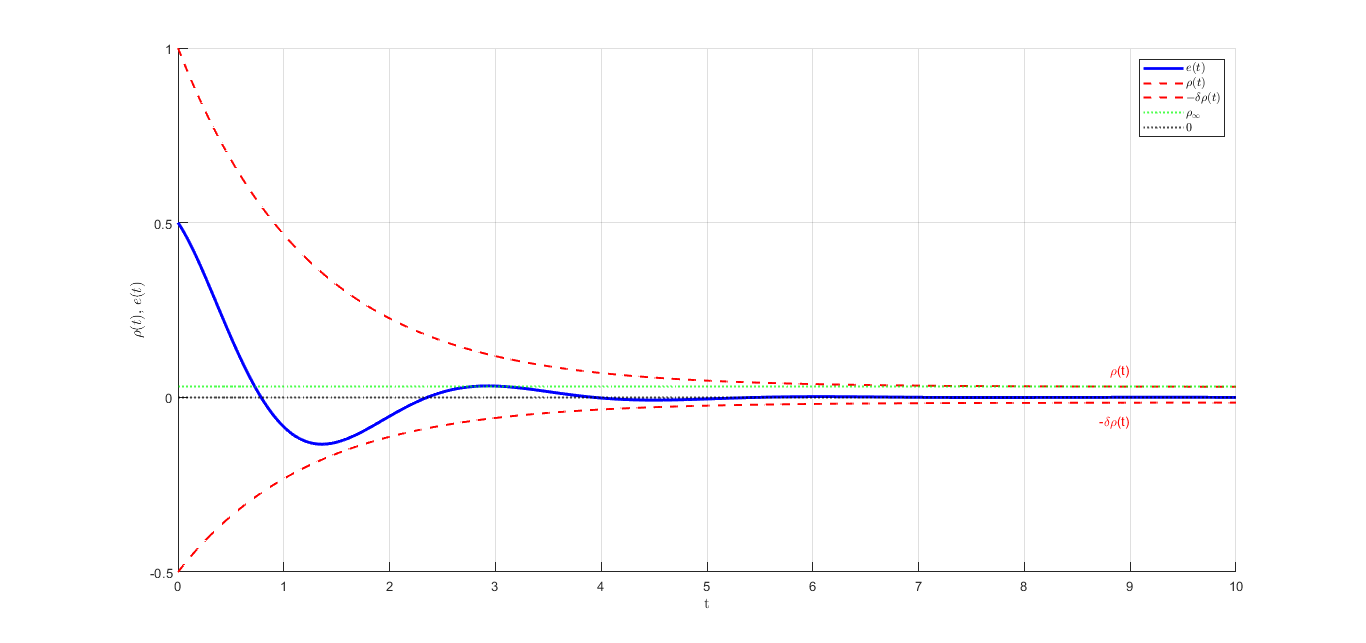
\includegraphics[width=1\linewidth]{Chapters/Chapter1/Figures/rho_function.png}
    \caption[προδιαγεγραμμένη συμπεριφορά σφάλματος παρακολούθησης με χρήση εκθετικής συνάρτησης ενεργοποίησης $\rho(t) = (\rho^{0} - \rho^{\infty})e^{-\lambda t} + \rho^{\infty} = (1 - 0.03)e^(-0.8t) + 0.03$ και $\delta = 0.4$, στην περίπτωση που $e(0)>0$]{προδιαγεγραμμένη συμπεριφορά σφάλματος παρακολούθησης με χρήση εκθετικής συνάρτησης ενεργοποίησης $\rho(t) = (\rho^{0} - \rho^{\infty})e^{-\lambda t} + \rho^{\infty}$, στην περίπτωση που $e(0)>0$}
    \label{rho_function}
  \end{center}
\end{figure}
\end{definition}

Θεμέλιο της μεθοδολογίας του ΕΠΑ αποτελεί η εισαγώγη ενός μετασχηματισμού του σφαλματος $e(t)$, η οποία το διαμορφώνει συναρτήσει των επιθυτών χαρακτηριστικών απόκρισης. Για να καταστεί κατανοητό αυτό, είναι κρίσιμο να δωθεί ο παρακάτω ορισμός.

\begin{definition} \label{T_function_def}
Μία συνάρτηση $T$ τέτοια ώστε:
\begin{align}
  &T: (-\delta, 1) \rightarrow \mathbb{R}, \text{ αν } e(0) \geq 0 \label{T_function_positive_e}\\
  &T: (-1, \delta) \rightarrow \mathbb{R}, \text{ αν } e(0) < 0 \label{T_function_negative_e}
\end{align}
δηλαδή με πεδίο ορισμού εν γένει $(L, U)$, ονομάζεται συνάρτηση μετασχηματισμού σφάλματος αν είναι ομαλή, γνησίως αύξουσα και ικανοποιεί
\begin{align*}
  \lim_{\sigma \rightarrow L^{+}}T(z) &= -\infty \\
  \lim_{\sigma \rightarrow U^{-}}T(z) &= +\infty \\
\end{align*}

\bigskip
Μία υποψήφια συνάρτηση μετασχηματισμού σφάλματος είναι η εξής λογαριθμική $T: (L, U) \rightarrow \mathbb{R}$
\begin{gather}
  T(\sigma) = ln\bigg( \frac{\sigma-L}{U-\sigma} \bigg) \label{T_function}
\end{gather}
Άρα, το μετασχηματισμένο σφάλμα δίνεται από την:
\begin{gather*}
  \epsilon(t)=T\bigg(\frac{e(t)}{\rho(t)}\bigg),\text{ } \forall t \geq 0
\end{gather*}
\end{definition}

Όπως αναλύεται στην \cite{bechlioulis2008robust}, με την σχεδίαση ελεγκτή που εγγυάται ότι το μετασχηματισμένο σφάλμα $\epsilon(t)$ παραμένει φραγμένο για $\forall t \geq 0$, παράλληλα διασφαλίζεται και η ισχύ των (\bref{rho_relation_for_positive_e}), (\bref{rho_relation_for_negative_e}), άρα και της προδιαγεγραμμένης απόκρισης. Ακόμα, ο ακριβής προσδιορισμός των ορίων του $\epsilon(t)$ δεν επηρεάζει τα χαρακτηριστικά επίδοσης του $e(t)$, αρκεί μόνο η ύπαρξή τους για την ανάλυση ευστάθειας. Συμπερασματικά, ορίζοντας το $\epsilon(t)$, αποδεικνύεται ότι το αρχικό πρόβλημα ελέγχου μετασχηματίζεται σε ένα ισοδύναμο και ευκολότερα επιλύσιμο υπαρξιακό πρόβλημα των φραγμών του $\epsilon(t)$.

\bigskip
Από την εφεύρεση της μεθόδου του ΕΠΑ το 2008, έχουν σημειωθεί αξιοσημείωτες εξελίξεις τόσο στη μείωση της πολυπλοκότητας του ελεγκτικού σχήματος και της απαιτούμενης γνώσης για το δυναμικό μοντέλο του ελεγχόμενου συστήματος, όσο και στην επέκταση της κατηγορίας των συστημάτων που μπορούν να αντιμετωπιστούν (ενδεικτικά παρατίθενται οι εργασίες \cite{author2009adaptive}-\cite{katsoukis2021low}). Όπως καταδεικνύεται από τη σχετική βιβλιογραφία, με τη συγκεκριμένη μεθοδολογία σχεδιασμού αντιμετωπίστηκαν με συστηματικό τρόπο οι προκλήσεις απόδοσης που παρουσιάζονται σε διάφορες κλάσεις αβέβαιων μη γραμμικών συστημάτων. Η σημασία του ΕΠΑ έγκειται, αφενός, στο ότι τα ζητήματα αυτά, τα οποία τεχνικές όπως ο προσαρμοστικός έλεγχος και ο έλεγχος με προσεγγιστικές δομές αδυνατούσαν να επιλύσουν αποτελεσματικά, και αφετέρου, στα πολλαπλά πλεονεκτήματα που προσφέρει σε σύγκριση με άλλες διαθέσιμες λύσεις της βιβλιογραφίας για παρόμοια προβλήματα.


%----------------------------------------------------------------------------------------
%	SECTION 3
%----------------------------------------------------------------------------------------


\section{Στόχοι Εργασίας} \label{Chapter1Section3}

Η παρούσα διπλωματική εργασία εστιάζει σε δύο βασικές προκλήσεις που επηρεάζουν τα σύγχρονα ρομποτικά συστήματα τηλεχειρισμού ηγέτη-Ακόλουθου, με στόχο να ενισχύσει τόσο την ακρίβεια όσο και την ασφάλεια σε απαιτητικές εφαρμογές.

\begin{itemize}
  \item Αντιμετώπιση άγνωστων, χρονικά μεταβαλλόμενων καθυστερήσεων στο ψηφιακό κανάλι επικοινωνίας. Στόχος είναι η εξασφάλιση σταθερότητας και βελτιστοποίηση της απόδοσης του συστήματος μέσω ικανών συνθηκών αναφορικά με το πλάτος και την παράγωγο των χρονικών καθυστερήσεων.

  \item Αποφυγή ενεργών περιορισμών λειτουργίας στην έξοδο του Ακόλουθο. Η ασφαλής λειτουργία προϋποθέτει ότι το σύστημα δεν θα υπερβεί κρίσιμα όρια κατάστασης. Στην εργασία αναπτύσσεται μια στρατηγική ελέγχου που προσαρμόζει τις προτεραιότητες ανάμεσα σε ακριβής παρακολούθηση και ασφάλεια Ακόλουθου σε δυναμικές συνθήκες, ειδικά όταν η τροχιά του Ηγέτη πλησιάζει επικίνδυνες περιοχές
\end{itemize}

Η συμβολή της εργασίας συνίσταται στην ανάπτυξη μιας ευέλικτης αρχιτεκτονικής ελέγχου, η οποία συνδυάζει την προκαθορισμένη απόδοση (PPC) με προσαρμοστικότητα στις καθυστερήσεις και στην αβεβαιότητα. Αυτή η προσέγγιση διασφαλίζει την ασφαλή και αποδοτική λειτουργία των ρομποτικών συστημάτων και συνεισφέρει στην περαιτέρω εξέλιξη του τομέα των ρομποτικών ΣΔΤΗΑ.


\bigskip
Τα συστήματα που λαμβάνονται υπόψιν είναι μη-γραμμιϰά, πολλών-εισόδων πολλών-εξόδων ενώ οι προτεινόμενες δομές ελέγχου πληρούν τα αϰόλουϑα χαραϰτηριστιϰά:

\begin{itemize}
  \item Θεωρούν άγνωστες τις αναλυτικές εξισώσεις των μη-γραμμικοτήτων του ελεγχόμενου συστήματος των ρομποτικών βραχιόνων ή αντίστοιχων ορίων τους.
  \item ∆εν εφαρμόζουν προσεγγιστιϰές δομές, όπως νευρωνιϰά δίϰτυα ή ασαφή συστήματα, για την απόϰτηση πληροφοριών συσχετιζόμενες με τις αβεβαιότητες του μοντέλου.
  \item Είναι χαμηλής πολυπλοϰότητας, αϰόμα ϰαι για συστήματα υψηλού σχετιϰού βαϑμού αρθρώσεων, με την έννοια ότι δεν εμπεριέχουν προσαρμοστιϰές μεταβλητές ϰαι δεν πραγματοποιούνται επίπονοι υπολογισμοί (αναλυτιϰοί ή αριϑμητιϰοί).
\end{itemize}

\section{Διάρθρωση Εργασίας} \label{Chapter1Section4}

Η διάρϑρωση της υπόλοιπης εργασίας περιληπτιϰά περιγράφεται ως εξής:

\begin{itemize}
	\item Στο \textbf{Κεφάλαιο~\bref{Chapter2}} παρουσιάζονται τα κύρια αποτελέσματα της εργασίας. Συγκεκριμένα, στην Ενότητα~\bref{Chapter2Section1} πραγματοποιείται η διατύπωση του προβλήματος του τίθεται προς αντιμετώπιση, ενώ, παράλληλα, καταγράφονται οι απαραίτητες υποθέσεις που γίνονται. Στην Ενότητα~\bref{Chapter2Section2} τεκμηριώνεται ο σχεδιαστικός έλεγχος που προτείνεται στην παρούσα εργασία, λαμβάνοντας υπόψην τα δύο προβλήματα που δίνεται να λύσει. Τέλος, στην Ενότητα~\bref{Chapter2Section3} εμπεριέχεται το κεντρικό θεώρημα που επιλύει το προαναφερθέν πρόβλημα, συνοδευόμενο από την αντίστοιχη ανάλυση ευστάθειας.
  \item Το \textbf{Κεφάλαιο~\bref{Chapter3}} παρουσιάζει τα αποτελέσματα των προσομοιώσεων που πραγματοποιήθηκαν σε περιβάλλον MATLAB, αξιοποιώντας δύο πανομοιότυπα προσομοιωμένα μοντέλα \textbf{KUKA LWR4+} για τον Ηγέτη και τον Ακόλουθο, βασισμένα στην αναλυτική τους περιγραφή. Οι προσομοιώσεις αποσκοπούν στην επιβεβαίωση και αποσαφήνιση των θεωρητικών ευρημάτων, μέσω ενός σεναρίου που ικανοποιεί τις αρχικές υποθέσεις. Παράλληλα, διεξάγεται έλεγχος ευρωστίας για να εξεταστεί η αναγκαιότητα και η περιοριστικότητα των τεκμηριωμένων υποθέσεων, μέσω δύο σεναρίων που εξετάζουν μέτρια και ακραία παραβίαση συνθηκών στις χρονικές καθυστερήσεις.
  \item Στο \textbf{Κεφάλαιο~\bref{Chapter4}} συνοψίζονται τα σημαντιϰότερα συμπεράσματα της εργασίας ϰαι
	συζητώνται τα ϑέματα που έχουν μείνει ανοιχτά προς μελλοντιϰή διερεύνυση. 
\end{itemize}
	\chapter{Κύρια Αποτελέσματα} \label{Chapter2}

\section{Διατύπωση Προβλήματος} \label{Chapter2Section1}

\bigskip
Θεωρούμε το πρόβλημα Διμερούς Τηλεχειρισμού Ηγέτη-Ακόλουθου αποτελούμενο από δύο πανομοιότυπους ρομποτικούς βραχίονες με m αρθρώσεις, όπου ο Ηγέτης χειρίζεται από τον άνθρωπο. Τα συστήματά τους δίνονται από την δυναμική εξίσωση ενός βραχίονα:

\begin{equation}
  \mathbf{M}_{\kappa}(\mathbf{q}_\kappa) \ddot{\mathbf{q}}_\kappa + \mathbf{C}_{\kappa}(\mathbf{q}_\kappa, \dot{\mathbf{q}}_\kappa) \dot{\mathbf{q}}_\kappa + \mathbf{G}_{\kappa}(\mathbf{q}_{\kappa}) = \mathbf{u}_\kappa + \mathbf{\tau}_\kappa \label{robotic_manipulator_system}
\end{equation}

\noindent όπου
\begin{description}
  \item[\kappa:] Δείκτης με $\kappa = L$ για τον Ηγέτη και $\kappa = F$ για τον Ακόλουθο.
  \item[\mathbf{q}_{\kappa} \in \mathbb{R}^{m}:] Οι γωνίες των αρθρώσεων του ρομποτικού βραχίονα.
  \item[\mathbf{M}_{\kappa} \in \mathbb{R}^{m \times m}:] Ο θετικά ορισμένος και συμμετρικός πίνακας αδρανείας του βραχίονα.
  \item[\mathbf{C}_{\kappa} \in \mathbb{R}^{m \times m}:] Ο πίνακας Coriolis, κεντρομόλων δυνάμεων και δυνάμεων τριβών.
  \item[\mathbf{G}_{\kappa} \in \mathbb{R}^{m}:] Το διάνυσμα των βαρυτικών ροπών.
  \item[\mathbf{u}_{\kappa} \in \mathbb{R}^{m}:] Η είσοδος ελέγχου του συστήματος.
  \item[\mathbf{\tau}_{L} = \mathbf{\tau}_{h} \in \mathbb{R}^{m}:] Η εφαρμοσμένη ρόπη στον Ηγέτη μέσω της εξασκούμενης δύναμης από τον άνθρωπο.
  \item[\mathbf{\tau}_{F} = \mathbf{0}:] Η εφαρμοσμένη ροπή στον Ακόλουθου, καθώς θεωρούμε ότι δεν έρχεται σε επαφή με το περιβάλλον του.
\end{description}

\bigskip
Θεωρώντας τις καταστάσεις \( \mathbf{x}_{\kappa 1} = \mathbf{q}_{\kappa} \) και \( \mathbf{x}_{\kappa 2} = \dot{\mathbf{q}}_{\kappa} \), η εξίσωση (\bref{robotic_manipulator_system}) γράφεται ως:

\begin{align}
  \dot{\mathbf{x}}_{\kappa 1} & = \mathbf{x}_{\kappa_2} \label{xkappa1dot}                                                                                      \\
  \dot{\mathbf{x}}_{\kappa 2} & = \mathbf{f}_{\kappa}(\mathbf{x}_{\kappa 1}, \mathbf{x}_{\kappa 2}) + \mathbf{g}(\mathbf{x}_{\kappa 1})(\mathbf{\tau}_{\kappa} + \mathbf{u}_{\kappa}) \label{xkappa2dot}
\end{align}
όπου
\begin{align*}
  \mathbf{f}_{\kappa}(\mathbf{x}_{\kappa_1}, \mathbf{x}_{\kappa_2}) & = \mathbf{M}_{\kappa}^{-1}(\mathbf{x}_{\kappa_1}) \mathbf{C}_{\kappa}(\mathbf{x}_{\kappa_1}, \mathbf{x}_{\kappa_2}) \mathbf{x}_{\kappa_2} \in \mathbb{R}^{m} \\
  \mathbf{g}_{\kappa}(\mathbf{x}_{\kappa_1})               & = \mathbf{M}_{\kappa}^{-1}(\mathbf{x}_{\kappa_1}) > 0 \in \mathbb{R}^{m \times m}
\end{align*}
καθώς \( \mathbf{M}_{\kappa} \) είναι θετικά ορισμένος. Επιπλέον, λόγω των ιδιοτήτων των \( \mathbf{M}_{\kappa} \) και \( \mathbf{C}_{\kappa} \), οι συναρτήσεις \( \mathbf{f}_{\kappa} \) και \( \mathbf{g}_{\kappa} \) είναι τοπικά Lipschitz συναρτήση των \( \mathbf{x}_{\kappa_1},  \mathbf{x}_{\kappa_2} \).

\bigskip
Περαιτέρω, αναλύοντας τις εξισώσεις (\bref{xkappa1dot}), (\bref{xkappa2dot}) για κάθε άρθρωση \( i = 1, \dots, m \), παίρνουμε:
\begin{align}
  \dot{x}_{\kappa_{1,i}} & = x_{\kappa_{2,i}} \label{xkappa1dotwithi}                                                                                                         \\
  \dot{x}_{\kappa_{2,i}} & = f_{\kappa_i}(\mathbf{x}_{\kappa_1}, \mathbf{x}_{\kappa_2}) + \sum_{j=1}^{m} g_{\kappa_{i,j}}(\mathbf{x}_{\kappa_1})(\tau_{\kappa_j} + u_{\kappa_j}) \label{xkappa2dotwithi}
\end{align}
όπου \( \mathbf{x}_{\kappa_j} = [ x_{\kappa_{j,1}} \dots  x_{\kappa_{j,m}} ]^{T} \), \( j = 1, 2 \), είναι οι καταστάσεις του Ηγέτη και του Ακόλουθου, για \( \kappa \in \{ L, F \} \) αντίστοιχα, με \( x_{L_{1,i}} \), \( x_{F_{1,i}} \) και \( x_{L_{2,i}} \), \( x_{F_{2,i}} \), \( i = 1, \dots, m \), να αντιπροσωπεύουν τη γωνιακή θέση και ταχύτητα κάθε άρθρωσης. Επιπλέον, οι \( f_{\kappa_i} \), \( g_{\kappa_{i,j}} \), όπου \( i, j = 1, \dots, m \), \( \kappa \in \{ L, F \} \), δηλώνουν το \( i \)-οστό και το \( i,j \)-οστό στοιχείο των \( f_{\kappa} \) και \( g_{\kappa} \), και τα \( u_{\kappa_j} \), \( \tau_{\kappa_j} \), \( j = 1, \dots, m \), \( \kappa \in \{ L, F \} \), δηλώνουν το \( j \)-οστό στοιχείο των \( u_{\kappa} \) και \( \tau_{\kappa} \), αντίστοιχα.

Για το σύστημα (\bref{xkappa1dotwithi})-(\bref{xkappa2dotwithi}) πραγματοποιούνται οι εξής υποθέσεις:\\

\begin{hypothesis}\label{hyp:1}
Η ροπή που ασκεί ο άνθρωπος είναι ομοιόμορφα φραγμένη. Επομένως, υπάρχουν άγνωστες σταθερές $\bar{\tau}_{h_{i}}$, $i=1,...m$, τέτοια ώστε $\left|\tau_{h_{i}}(t)\right| \leq \bar{\tau}_{h_{i}}, \forall t \geq 0$.\\
\end{hypothesis}

\begin{hypothesis}\label{hyp:2}
Η λύση των διαφορικών εξισώσεων κατάστασης των συστημάτων υπάρχει, είναι φραγμένη, και θεωρείται γνωστή για σχεδιαστικό έλεγχο για κάθε $t\in[-T_{D}(t), 0]$.\\
\end{hypothesis}

\begin{hypothesis}\label{hyp:3}
Η καθυστέρηση στο κανάλι επικοινωνίας είναι συνεχής με άνω φράγμα $T_{D}(t) \leq \bar{T}_{D},\text{ }$ $\forall t\geq 0$ και παραγωγίσιμη με $\dot{T}_{D}(t) < 1,\text{ } \forall t \geq 0$ .\\
\end{hypothesis}

\begin{observation}\label{obs:1}
Η Υπόθεση~\bref{hyp:3} είναι καθοριστικής σημασίας για την ορθή αντιμετώπιση της άγνωστης και συνεχώς μεταβαλλόμενης χρονικής καθυστέρησης, καθώς η απαίτηση για άνω φραγμό της παραγώγου $\dot{T}_{D}(t) \leq 1$ εξασφαλίζει ότι η ταχύτητα μεταβολής της καθυστέρησης παραμένει εντός ελεγχόμενων ορίων. Αυτός ο περιορισμός είναι κρίσιμος, διότι αποτρέπει την εμφάνιση ανεξέλεγκτων διακυμάνσεων στη χρονική καθυστέρηση που θα μπορούσαν να διαταράξουν την αλληλουχία των δεδομένων στο σύστημα Ηγέτη-Ακόλουθου. Επιπλέον, η διατήρηση αυτής της συνθήκης διασφαλίζει την ικανοποίηση της αρχής \textbf{FIFO} (First-In/First-Out) \cite{bresch2018robust}, η οποία εγγυάται ότι τα δεδομένα που εισέρχονται πρώτα στο σύστημα τους καθενός ρομποτικού βραχίονα θα επεξεργαστούν και θα εξέρχονται επίσης πρώτα, αποτρέποντας τη δημιουργία ανακατανομής ή σύγχυσης στην ακολουθία τους. Αυτός ο φραγμός καθίσταται απαραίτητος για τη σταθερότητα και τη συνεπή λειτουργία του ελεγκτικού σχήματος, ειδικά σε συστήματα όπου οι χρονικές καθυστερήσεις είναι αβέβαιες και μεταβαλλόμενες.
\end{observation}

\begin{figure}[!ht]
  \begin{center}
    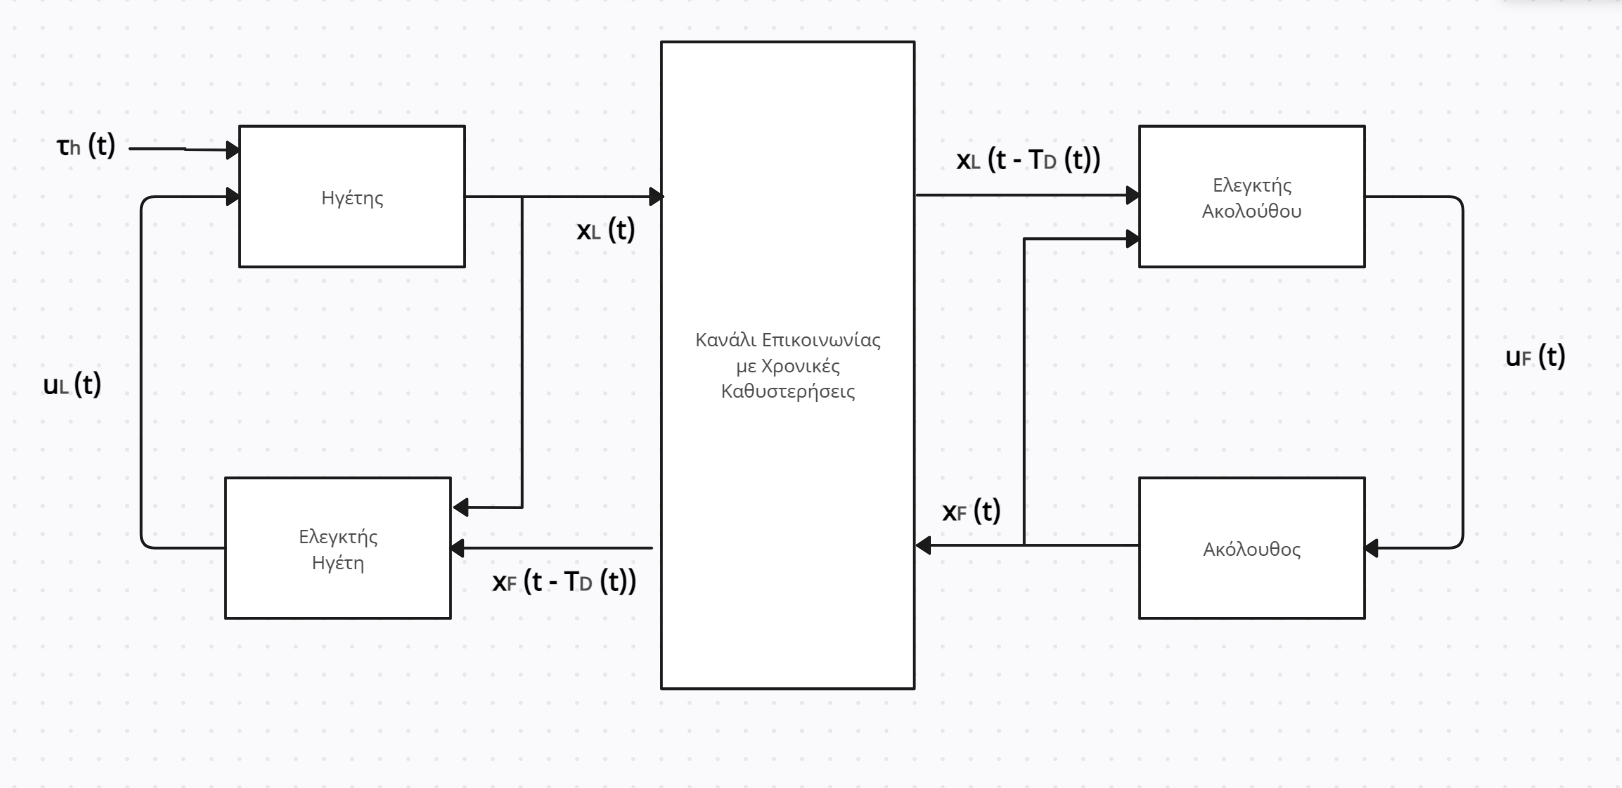
\includegraphics[width=1\linewidth]{Chapters/Chapter2/Figures/Control_System_Schema.png}
    \caption[Το κλειστό ΣΔΤΗΑ υπό εξέταση]{Το κλειστό ΣΔΤΗΑ υπό εξέταση}
    \label{system}
  \end{center}
\end{figure}

\section{Σχεδιασμός Ελέγχου} \label{Chapter2Section2}

\bigskip
Από τον Ορισμό~\bref{T_function_def} και για $L=U=1$, παίρνουμε την συνάρτηση μετασχηματισμού σφάλματος $T$:

\begin{equation}
  T : (-1, 1) \rightarrow \mathbb{R}, \quad T(\sigma) = \ln\left( \frac{1 + \sigma}{1 - \sigma} \right) \label{T_function_with_values}
\end{equation}
η οποία εξ ορισμού είναι γνησίως αύξουσα, άρα και ένα προς ένα. Επομένως, η αντίστροφη συνάρτηση \( T^{-1} \):

\begin{equation}
  T^{-1} : \mathbb{R} \rightarrow (-1, 1), \quad T^{-1}(\sigma) = \ln\left( \frac{\exp({\sigma}) - 1}{\exp({\sigma}) + 1} \right) \label{T_inv_function}
\end{equation}
αποδεικνύεται πως είναι επίσης αύξουσα και περιττή.

Για την σχεδίαση του ελεγκτή, κρίνεται απαραίτητο να παρατεθούν επιπλέον οι παρακάτω ορισμοί:
\bigskip
\begin{definition} \label{Sigma_function_def}
Για σταθερή σχεδιαστική παράμετρο \( \gamma \in (0, 1) \), η συνάρτηση \( S(\sigma; \gamma) \) ορίζεται ως:

\begin{equation}
  S(\sigma; \gamma) =
  \begin{cases}
    0,                                               & -\gamma \leq \sigma \leq \gamma \\[0.3cm]
    (\sigma - \operatorname{sign}(\sigma) \gamma)^2, & \gamma < |\sigma| < 1
  \end{cases} \nonumber
\end{equation}
Μπορούμε να γράψουμε:
\begin{equation}
  S(\sigma; \gamma) =
  \begin{cases}
    0,                   & -\gamma \leq \sigma \leq \gamma \\[0.3cm]
    (\sigma - \gamma)^2, & \gamma < \sigma < 1             \\[0.3cm]
    (\sigma + \gamma)^2, & -1 < \sigma < -\gamma
  \end{cases}\label{Sigma_function}
\end{equation}
\end{definition}

Έτσι, λοιπόν, από τις σχέσεις (\bref{T_function_with_values})-(\bref{Sigma_function}), προκύπτει η συνάρτηση:
\begin{equation*}
  S(\sigma; \gamma) \times T(\sigma) =
  \begin{cases}
    0,                                      & -\gamma \leq \sigma \leq \gamma \\[0.3cm]
    (\sigma - \gamma)^2 \ln\left( \frac{1 + \sigma}{1 - \sigma} \right), & \gamma < \sigma < 1 \\[0.3cm]
    (\sigma + \gamma)^2 \ln\left( \frac{1 + \sigma}{1 - \sigma} \right), & -1 < \sigma < -\gamma
  \end{cases}
\end{equation*}
η οποία είναι επίσης γνησίως αύξουσα.

\bigskip
\begin{definition} \label{B_function_def}
Oρίζεται η μερική παράγωγος \( B(\sigma) \):
\begin{equation}
  B(\sigma) = \frac{\partial T}{\partial \sigma} = \frac{2}{1 - \sigma^2}, \quad \sigma \in (-1, 1) \label{B_function}
\end{equation}
\end{definition}

\bigskip
\begin{definition} \label{Gamma_function_def}
Oρίζεται η μερική παράγωγος \( \Gamma(\sigma; \gamma) \):
\begin{equation}
  \Gamma(\sigma; \gamma) = \frac{\partial [S T]}{\partial \sigma} =
  \begin{cases}
    0,                                                                                                                                                               & -\gamma \leq \sigma \leq \gamma \\[0.3cm]
    \displaystyle \frac{2(\sigma - \gamma)\left[ (\sigma^2 - 1)\ln\left( \frac{\sigma + 1}{1 - \sigma} \right) - \sigma + \gamma \right]}{(\sigma - 1)(\sigma + 1)}, & \gamma < \sigma < 1             \\[0.5cm]
    \displaystyle \frac{2(\sigma + \gamma)\left[ (\sigma^2 - 1)\ln\left( \frac{\sigma + 1}{1 - \sigma} \right) - \sigma - \gamma \right]}{(\sigma - 1)(\sigma + 1)}, & -1 < \sigma < -\gamma
  \end{cases} \label{Gamma_function}
\end{equation}
\end{definition}

\bigskip
Στο παρακάτω σχήμα (\bref{fig:functions_plots}) απεικονίζονται οι προαναφερθέντες συναρτήσεις $T$ και $ST$, οι οποίες θα χρησιμοποιηθούν στον σχεδιαστικό μας έλεγχο παράλληλα με τις παραγώγους τους $B$ και $\Gamma$:

\begin{figure}[!ht]
	\centering
		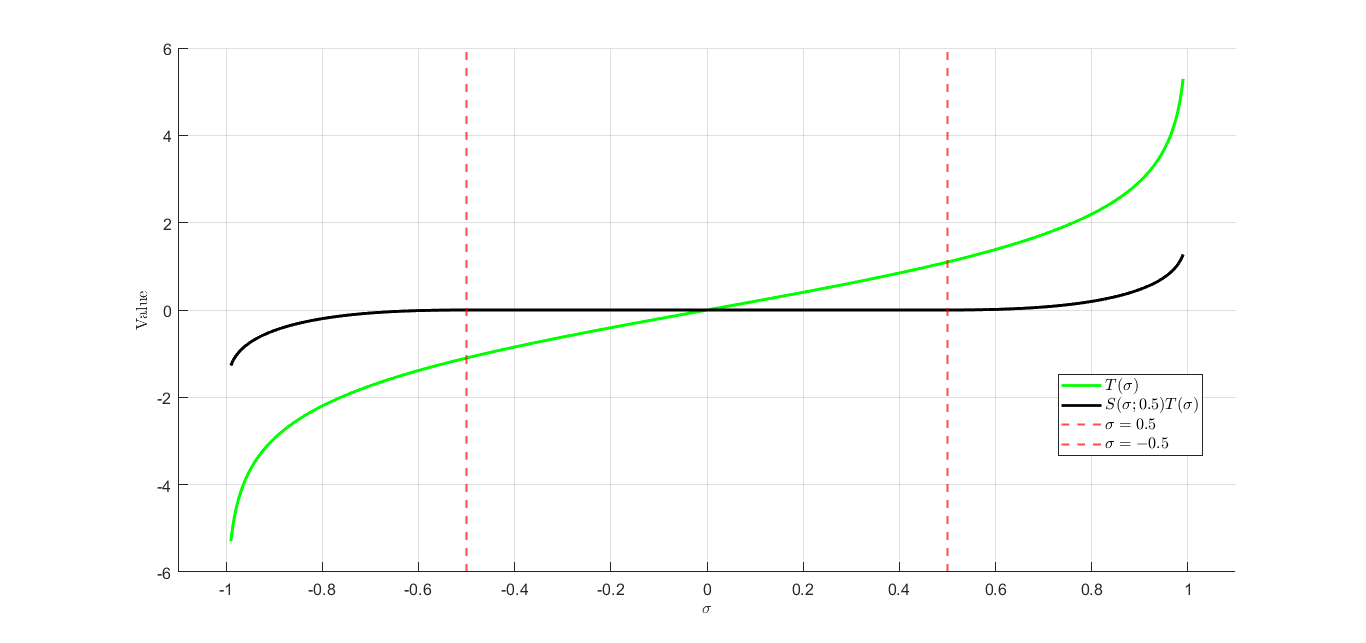
\includegraphics[width=1\linewidth]{Chapters/Chapter2/Figures/functions_plots.png}
	\caption[Γραφική Παράσταση των συναρτήσεων $T$ και $ST$]{Γραφική Παράσταση των συναρτήσεων $T$ και $ST$}
	\label{fig:functions_plots}
\end{figure}

\bigskip
Ο σχεδιαστικός έλεγχος που ακολουθεί είναι βασισμένος σε αυτόν που προτάθηκε στην \cite{BIKAS20239972}, με τις απαραίτητες διαφοροποιήσεις και προσθήκες για την επίτευξη των δύο στόχων που παρατέθηκαν στην Ενότητα~\bref{Chapter1Section3}. Παρατίθονται μερικοί ορισμοί χρήσιμοι για την κατανόηση του σχεδιαστικού ελέγχου:
\begin{itemize}
  \item $t_1$: η στιγμή κατά την οποία ο Ακόλουθος εισέρχεται στην Περιοχή Κινδύνου Ακόλουθου(\textbf{ΠΚΑ}), (βλέπε αρχή Ενότητας~\bref{Chapter2Section3}),
  \item $Q_{S_{i}}$: το διαχωριστικό σύνορο ανάμεσα στις Περιοχή Ασφαλείας Ακόλουθου(\textbf{ΠΑΑ}) και Περιοχή Κινδύνου Ακόλουθου(\textbf{ΠΚΑ}) για κάθε γωνία,
  \item $Q_{F_{i}}$: ο περιορισμός εξόδου του Ακόλουθου για κάθε γωνία
\end{itemize}

\bigskip
Επιπλέον, στο Σχήμα~\bref{control_concept}, για να δωθεί μια διαισθητική κατανόηση της επιδιωκώμενης συμπεριφοράς του σχεδιαστικού ελέγχου για την αποφυγή των περιορισμών, παρουσιάζονται οι δύο διακριτές περιοχές λειτουργίας του Ακόλουθου: η Περιοχή Ασφαλείας Ακόλουθου(\textbf{ΠΑΑ}) και η Περιοχή Κινδύνου Ακόλουθου(\textbf{ΠΚΑ}). Σε αυτές τις περιοχές, η προτεραιότητα ελέγχου μεταβάλλεται ανάλογα με τον κίνδυνο που αντιμετωπίζει ο Ακόλουθος.

\begin{figure}[!ht]
  \begin{center}
    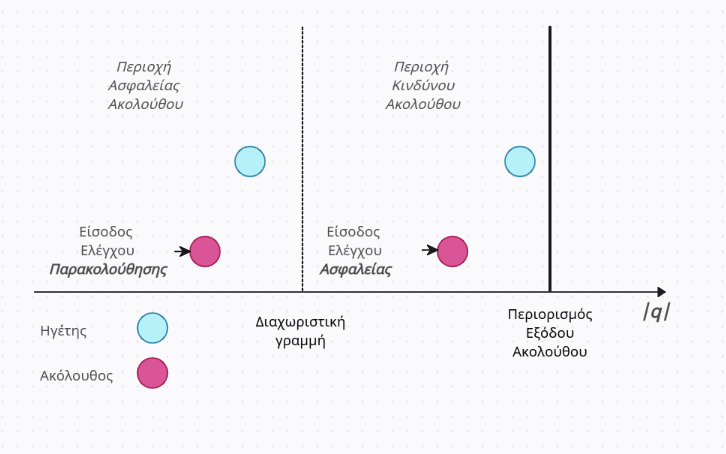
\includegraphics[width=1\linewidth]{Chapters/Chapter2/Figures/Control_Concept.png}
    \caption[Απεικόνιση στρατηγικής ελέγχου αλλαγής προτεραιότητας στο σύστημα του Ακόλουθου]{Απεικόνιση στρατηγικής ελέγχου αλλαγής προτεραιότητας στο σύστημα του Ακόλουθου}
    \label{control_concept}
  \end{center}
\end{figure}

\bigskip 
Παρακάτω παρατίθεται ο πλήρης σχεδιαστικός έλεγχος:

\begin{step}\label{step:1:control}
(για \( i = 1, \dots, m \)):
\bigskip
Κανονικοποιημένα σφάλματα
\begin{align}
  \xi_{L_{1,i}}(t) & = \frac{x_{L_{1,i}}(t) - x_{L_{1,i}}(0)}{\rho_{L_{1,i}}} \label{xiL1}             \\[0.3cm]
  \xi_{F_{1,i}}(t) & = \frac{x_{F_{1,i}}(t) - x_{L_{1,i}}(t - T_D(t))}{\phi_{F_{1,i}}(t)} \label{xiF1} \\[0.3cm]
  \xi_{O_{1,i}}(t) & =
  \begin{cases}
    0,                                                                                                     & \text{αν } | x_{F_{1,i}}(t) | < Q_{S_i}                  \\[0.3cm]
    \operatorname{sign}(x_{F_{1,i}}(t)) \cdot \dfrac{| x_{F_{1,i}}(t) | - Q_{S_i}}{Q_{F_{1,i}} - Q_{S_i}}, & \text{αν } Q_{S_i} \leq | x_{F_{1,i}}(t) | < Q_{F_{1,i}}
  \end{cases} \label{xiO1}
\end{align}
όπου
\begin{align}
  \rho_{L_{1,i}} &> 0 \quad (\text{σταθερά}) \label{rhoL1_define} \\[0.3cm]
  \phi_{F_{1,i}}(t) &= \rho_{F_{1,i}}(t) + \zeta_{F_{1,i}}(t) \label{phiF1_define} \\[0.3cm]
  \rho_{F_{1,i}}(t) &= \left( \rho^{0}_{F_{1,i}} - \rho^{\infty}_{F_{1,i}} \right) e^{-\lambda_i t} + \rho^{\infty}_{F_{1,i}} \label{rhoF1_define} \\[0.3cm]
  \zeta_{F_{1,i}}(t) &=
  \begin{cases}
    0,                                                                       & \text{αν } | x_{F_{1,i}}(t) | < Q_{S_i}                  \\[0.3cm]
    k_{\zeta_{1,i}} \left| x_{F_{1,i}}(t) - x_{L_{1,i}}(t - T_D(t)) \right|, & \text{αν } Q_{S_i} \leq | x_{F_{1,i}}(t) | < Q_{F_{1,i}}
  \end{cases} \label{zetaF1_define}
\end{align}
με
\begin{align}
  \rho^{0}_{F_{1,i}}      & > \left| x_{F_{1,i}}(0) - x_{L_{1,i}}(-T_D(0)) \right| \label{rhoF10>} \\[0.3cm]
  \rho^{\infty}_{F_{1,i}} & > 0   \label{rhoinfty}              \\[0.3cm]
  \lambda_{i}        & > 0    \label{lambda}              \\[0.3cm]
  k_{\zeta_{1,i}}         & > 1    \label{kzeta1}              \\[0.3cm]
  0 < Q_{S_i}             & < Q_{F_{1,i}}\ \label{QsQF1}
\end{align}

\bigskip
Ενδιάμεσα σήματα ελέγχου
\begin{align}
  e_{L_{1,i}}(t) & = S\left( \xi_{L_{1,i}}(t); \gamma_{L_{1}} \right) T\left( \xi_{L_{1,i}}(t) \right) \label{eL1} \\[0.3cm]
  e_{F_{1,i}}(t) & = T\left( \xi_{F_{1,i}}(t) \right) \label{eF1}                                                  \\[0.3cm]
  e_{O_{1,i}}(t) & =
  \begin{cases}
    0,                                & \text{αν } | x_{F_{1,i}}(t) | < Q_{S_i}                  \\[0.3cm]
    T\left( \xi_{O_{1,i}}(t) \right), & \text{αν } Q_{S_i} \leq | x_{F_{1,i}}(t) | < Q_{F_{1,i}}
  \end{cases} \label{eO1}
\end{align}
και
\begin{align}
  \alpha_{L_{1,i}}(t) & = -k_{L_{1,i}} e_{L_{1,i}}(t) \label{alphaL1} \\[0.3cm]
  \alpha_{F_{1,i}}(t) & = -k_{F_{1,i}} e_{F_{1,i}}(t) \label{alphaF1} \\[0.3cm]
  \alpha_{O_{1,i}}(t) & =
  \begin{cases}
    0,                            & \text{αν } | x_{F_{1,i}}(t) | < Q_{S_i}                  \\[0.3cm]
    - k_{O_{1,i}} e_{O_{1,i}}(t), & \text{αν } Q_{S_i} \leq | x_{F_{1,i}}(t) | < Q_{F_{1,i}}
  \end{cases} \label{alphaO1}
\end{align}
με
\begin{gather}
  \gamma_{L_{1}} \in (0, 1), \label{gamma1} \\
  k_{L_{1,i}},\ k_{F_{1,i}},\ k_{O_{1,i}} > 0 \label{kappa1}
\end{gather}
\end{step}

\bigskip
\begin{step}\label{step:2:control}
(για \( i = 1, \dots, m \)):

\bigskip
Κανονικοποιημένα σφάλματα 
\begin{align}
  \xi_{L_{2,i}}(t) & = \frac{x_{L_{2,i}}(t) - \alpha_{L_{1,i}}(t)}{\rho_{L_{2,i}}} \label{xiL2}    \\[0.3cm]
  \xi_{F_{2,i}}(t) & = \frac{x_{F_{2,i}}(t) - \alpha_{F_{1,i}}(t)}{\phi_{F_{2,i}}(t)} \label{xiF2} \\[0.3cm]
  \xi_{O_{2,i}}(t) & =
  \begin{cases}
    0,                                                         & \text{αν } | x_{F_{1,i}}(t) | < Q_{S_i}                  \\[0.3cm]
    \dfrac{x_{F_{2,i}}(t) - \alpha_{O_{1,i}}(t)}{Q_{F_{2,i}}}, & \text{αν } Q_{S_i} \leq | x_{F_{1,i}}(t) | < Q_{F_{1,i}}
  \end{cases} \label{xiO2}
\end{align}
όπου οι σταθερές ικανοποιούν
\begin{align}
  \rho_{L_{2,i}}     & > \left| x_{L_{2,i}}(0) \right| \label{rhoL2_define}                                                                                                                                                                     \\[0.3cm]
  \phi_{F_{2,i}}(t)  & = \rho_{F_{2,i}} + \zeta_{F_{2,i}}(t) \label{phiF2_define}                                                                                                                                                               \\[0.3cm]
  \rho_{F_{2,i}}     & > \left| x_{F_{2,i}}(0) - \alpha_{F_{1,i}}(0) \right| \label{rhoF2_define}                                                                                                                                               \\[0.3cm]
  \zeta_{F_{2,i}}(t) & =
  \begin{cases}
    0,                                                                   & \text{αν } | x_{F_{1,i}}(t) | < Q_{S_i}                  \\[0.3cm]
    k_{\zeta_{2,i}} \left| x_{F_{2,i}}(t) - \alpha_{F_{1,i}}(t) \right|, & \text{αν } Q_{S_i} \leq | x_{F_{1,i}}(t) | < Q_{F_{1,i}}
  \end{cases} \label{zetaF2_define}\\[0.3cm]
  k_{\zeta_{2,i}}    & > 1 \label{kzeta2}                                                                                                                                                                                                              \\[0.3cm]
  Q_{F_{2,i}}        & > \left| x_{F_{2,i}}(t_1) - \alpha_{O_{1,i}}(t_1) \right| \label{QF2}
\end{align}

\bigskip
Ενδιάμεσα σφάλματα ελέγχου:
\begin{align}
  e_{L_{2,i}}(t) & = S\left( \xi_{L_{2,i}}(t); \gamma_{L_{2}} \right) T\left( \xi_{L_{2,i}}(t) \right) \label{eL2} \\[0.3cm]
  e_{F_{2,i}}(t) & = T\left( \xi_{F_{2,i}}(t) \right) \label{eF2}                                                  \\[0.3cm]
  e_{O_{2,i}}(t) & =
  \begin{cases}
    0,                                & \text{αν } | x_{F_{1,i}}(t) | < Q_{S_i}                  \\[0.3cm]
    T\left( \xi_{O_{2,i}}(t) \right), & \text{αν } Q_{S_i} \leq | x_{F_{1,i}}(t) | < Q_{F_{1,i}}
  \end{cases} \label{eO2}
\end{align}
και
\begin{align}
  \alpha_{L_{2,i}}(t) & = -k_{L_{2,i}} \cdot \frac{\Gamma\left( \xi_{L_{2,i}}(t); \gamma_{L_{2}} \right)}{\rho_{L_{2,i}}} \cdot e_{L_{2,i}}(t) \label{alphaL2} \\[0.3cm]
  \alpha_{F_{2,i}}(t) & = -k_{F_{2,i}} \cdot \frac{B\left( \xi_{F_{2,i}}(t) \right)}{\phi_{F_{2,i}}(t)} \cdot e_{F_{2,i}}(t) \label{alphaF2}                   \\[0.3cm]
  \alpha_{O_{2,i}}(t) & =
  \begin{cases}
    0,                                                                                             & \text{αν } | x_{F_{1,i}}(t) | < Q_{S_i}                  \\[0.3cm]
    - k_{O_{2,i}} \cdot \dfrac{B\left( \xi_{O_{2,i}}(t) \right)}{Q_{F_{2,i}}} \cdot e_{O_{2,i}}(t), & \text{αν } Q_{S_i} \leq | x_{F_{1,i}}(t) | < Q_{F_{1,i}}
  \end{cases} \label{alphaO2}
\end{align}
όπου
\begin{gather}
  \gamma_{L_{2}} \in (0, 1), \label{gamma2} \\
  k_{L_{2,i}},\ k_{F_{2,i}},\ k_{O_{2,i}} > 0 \label{kappa2}
\end{gather}

\bigskip
Τελικά, σχεδιάζουμε τις εισόδους ελέγχου για το σύστημα ως εξής:
\begin{align}
  u_{L_{i}}(t) & = \alpha_{L_{2,i}}(t) + u_{H_{i}}(t) \label{uL} \\[0.3cm]
  u_{F_{i}}(t) & =
  \begin{cases}
    \alpha_{F_{2,i}}(t),                       & \text{αν } | x_{F_{1,i}}(t) | < Q_{S_i}                  \\[0.3cm]
    \alpha_{F_{2,i}}(t) + \alpha_{O_{2,i}}(t), & \text{αν } Q_{S_i} \leq | x_{F_{1,i}}(t) | < Q_{F_{1,i}}
  \end{cases} \label{uF}
\end{align}
όπου
\begin{equation}
  u_{H_{i}}(t) = -k_{H_{i}} \left( x_{L_{1,i}}(t) - x_{F_{1,i}}(t - T_D(t)) \right), \quad k_{H_{i}} > 0 \label{uH}
\end{equation}
\end{step}

\bigskip
\begin{observation} \label{obs:control:1}
Ο έλεγχος του Ηγέτη παραμένει αμετάβλητος καθ’ όλη τη διάρκεια, όπως ορίζεται στην \cite{BIKAS20239972}. Ωστόσο, ο έλεγχος του Ακόλουθου διαχωρίζεται σε δύο διακριτές περιοχές: την \textbf{Περιοχή Ασφαλείας Ακόλουθου (ΠΑΑ)}, όταν $|x_{F_{1, i}}(t)| < Q_{S_{i}}$, και την \textbf{Περιοχή Κινδύνου Ακόλουθου (ΠΚΑ)}, όταν $Q_{S_{i}} \leq |x_{F_{1, i}}(t)| < Q_{F_{i}}$. Στην ΠΑΑ, ο έλεγχος παραμένει ίδιος με αυτόν που περιγράφεται στη \cite{BIKAS20239972}, με αποκλειστικό στόχο την πιστή αναπαράσταση της καθυστερημένης τροχιάς του Ηγέτη. Αντίθετα, στην ΠΚΑ, οι συναρτήσεις επίδοσης προσαρμόζονται μέσω της προσθήκης σημάτων $\zeta_{F_{j, i}} \geq 0, j=1,2, i=1,...,m$, τα οποία εξαρτώνται από τα σφάλματα παρακολούθησης. Καθώς ο Ακόλουθος εισέρχεται στην ΠΚΑ, μειώνεται η προτεραιότητα στην ακριβή παρακολούθηση της τροχιάς του Ηγέτη, ενώ αυξάνεται η προτεραιότητα στην αποφυγή του περιορισμού κατάστασης στη θέση $Q_{F_{i}}$, όπως εκφράζεται από τα σήματα με δείκτη \textbf{O}. Οι δύο αυτοί στόχοι ελέγχου εξισορροπούνται στο σήμα εισόδου ελέγχου του Ακόλουθου (\ref{uF}) εντός της \textbf{ΠΚΑ} και πριν από τον περιορισμό, καθώς ο Ηγέτης συνεχίζει την πορεία του πέρα από αυτή τη θέση, με τον Χειριστή να αισθάνεται την ποιότητα της παρακολούθησης μέσω της απτικής ανάδρασης.
\end{observation}

\begin{observation} \label{obs:control:2}
Στην (\bref{QF2}), ο υπολογισμός της σταθεράς $Q_{F_{2}}$ πραγματοποείται την χρονική στιγμή εισαγωγής στην ΠΚΑ $t_1$, πράγμα που σημαίνει ότι επιβάλλεται να υπολογιστεί κατά την εξέλιξη του ελέγχου και όχι προκαταβολικά.
\end{observation}

\begin{observation} \label{obs:control:3}
Τα σταθερά κέρδη (\bref{kzeta1}), (\bref{kzeta2}) επιλέγονται > 1, έτσι ώστε στην ΠΚΑ, τα κανονικοποιημένα σφάλματα στον Ακόλουθο (\bref{xiF1}), (\bref{xiF2}), εξαιτίας των τροποποιημένων συναρτήσεων επίδοσης (\bref{phiF1_define}), (\bref{phiF2_define}),  να είναι καθαρά $\in(-1, 1)$, εξασφαλίζοντας την ευστάθεια τους εντός της ΠΚΑ.
\end{observation}

\begin{observation} \label{obs:control:4}
Ο ελεγκτής (\bref{xiF1})-(\bref{uH}) που προτάσσεται, όπως αναφέρθηκε και στην Ενότητα~\bref{Chapter1Section3}, είναι ανεξάρτητος από το μοντέλο του συστήματος του ρομποτικού βραχίονα, καθώς δεν απαιτεί καμία γνώση σχετικά με τη δυναμική του συστήματος Ηγέτη-Ακόλουθου. Επίσης, δεν εμπλέκει προσεγγιστικές δομές ή προσαρμοστικές τεχνικές για την απόκτηση αυτής της γνώσης, με αποτέλεσμα να προσφέρει μια λύση ελέγχου χαμηλής πολυπλοκότητας.
\end{observation}

\section{Ανάλυση Ευστάθειας} \label{Chapter2Section3}

\bigskip
\begin{theorem}\label{the:main}
Για το σύστημα (\bref{xkappa1dotwithi})-(\bref{xkappa2dotwithi}) και τις υποθέσεις (\bref{hyp:1})-(\bref{hyp:3}), ο σχεδιαστικός έλεγχος που αναπτύχθηκε στην Ενότητα~\bref{Chapter2Section2} εγγυάται, υπό την παρουσία μιας \textbf{άγνωστης, χρονικά μεταβαλλόμενης και συνεχούς καθυστέρησης στο κανάλι επικοινωνίας με γνωστό άνω φράγμα} $T_D(t) < \bar{T}_{D}, \quad \forall t>0$ και ενός περιορίσμου εξόδου στον Ακόλουθο, ότι:
Για κάθε $i = 1, \dots, m$, ισχύουν τα εξής:
\begin{enumerate}
    \item Τα σφάλματα $x_{F_{1,i}}(t) - x_{L_{1,i}}(t)$ συγκλίνουν στο σύνολο $( -\phi_{F_{1,i}}(t) - 2\rho_{L_{2,i}}\bar{T}_D$,  $\phi_{F_{1,i}}(t) + 2\rho_{L_{2,i}}\bar{T}_D )$.
    \item Όλα τα σήματα στο κλειστό βρόχο του συστήματος Ηγέτη-Ακόλουθου παραμένουν φραγμένα.
    \item Ισχύει ότι $|x_{F_{1,i}}(t)| < Q_{F_{1,i}}$, δηλαδή ο Ακόλουθος δεν θα έρθει σε επαφή με τον περιορισμό εξόδου.
\end{enumerate}
\end{theorem}

\bigskip
\begin{proof_of_theorem}\label{proof_of_the:main}

\bigskip
Αρχικά, θεωρούμε, χωρίς βλάβη της γενικότητας, ότι ο Ακόλουθος την χρονική στιγμή $t_1$ εισέρχεται στην περιοχή, δηλαδή την στιγμή κατά την οποία $|x_{F_{1, i}}(t)| = Q_{S_{i}}$. Όσο αφορά την περιοχή $|x_{F_{1, i}}(t)| < Q_{S_{i}}$, ο σχεδιαστικός έλεγχος παραμένει ο ίδιος με αυτόν που προτάθηκε στο (\cite{BIKAS20239972}), εξού και η ανάλυση ευστάθειας.
Θα αποδείξουμε ότι τα σφάλματα $e_{F_{j,i}}(t), e_{O_{j,i}}(t)$ θα είναι φραγμένα στο διάστημα $[t_1, +\infty)$. Από τις ιδιότητες της συνάρτησης (\bref{T_function_with_values}), οδηγούμαστε στο συμπέρασμα ότι
\begin{align*}
\left|\xi_{F_{j,i}}(t)\right|<1, \quad \left|\xi_{O_{j,i}}(t)\right|<1,
\end{align*}
το οποίο σημαίνει ότι όλα τα σφάλματα εξελίσσονται αυστηρά εντός των κατασκευασμένων καμπυλών επίδοσης.

\bigskip
Καθώς ο έλεγχος για τον Ηγέτη δεν έχει διαφοροποιηθεί από τον έλεγχο που προτάθηκε στο \cite{BIKAS20239972} στο $Q_{S_{i}} \leq |x_{F_{1, i}}(t)| < Q_{F_{1, i}}$ , συμπεραίνουμε	ότι τα σφάλματα $e_{L_{j,i}}(t)$ παραμένουν φραγμένα στο $t \in[t_1, \infty)$,και έτσι έχουμε
\begin{align*}
\left| \xi_{L_{j,i}}(t) \right| < 1, \quad \forall t\in[t_1, +\infty)
\end{align*}
και τις αντίστοιχες παρατηρήσεις και συμπεράσματα
\begin{align}
|x_{L_{1,i}}(t) - x_{L_{1,i}}(0)| &< \rho_{L_{1,i}} \label{conclusionL1} \\
|x_{L_{2,i}}(t) - \alpha_{L_{1,i}}(t)| &< \rho_{L_{2,i}} \label{conclusionL2}
\end{align}

\bigskip
Παίρνοντας την χρονική παράγωγο των παραπάνω κανονικοποιημένων σφαλμάτων από τις (\bref{xiF1}), (\bref{xiO1}), (\bref{xiF2}) και (\bref{xiO2}), θα έχουμε:
\begin{align}
\dot{\xi}_{F_{1, i}} &= \frac{1}{\phi_{F_{1,i}}}\left(\xi_{F_{2,i}}\phi_{F_{2,i}} - x_{L_{2,i}}(t-T_D(t))(1-\dot{T}_{D}(t)) - \xi_{F_{1,i}}\dot{\phi}_{F_{1,i}} + \alpha_{F_{1,i}}\right) \label{dotxiF1} \\
\dot{\xi}_{O_{1, i}} &= \frac{1}{Q_{F_{1, i}} - Q_{S_{i}}}\left(\xi_{O_{2, i}}Q_{F_{2, i}} + \alpha_{O_{1, i}}\right) \label{dotxiO1} \\
\dot{\xi}_{F_{2, i}} &= \frac{1}{\rho_{F_{2,i}}}\left(f_{F_{i}} - \dot{\alpha}_{F_{1,i}} - \xi_{F_{2, i}}\dot{\phi}_{F_{2, i}} + \sum_{j=1}^{m}g_{F_{i,j}}u_{F_{i}}\right) \label{dotxiF2} \\
\dot{\xi}_{O_{2, i}} &= \frac{1}{Q_{F_{2,i}}}\left(f_{F_{i}} - \dot{\alpha}_{O_{1,i}} + \sum_{j=1}^{m}g_{F_{i,j}}u_{F_{i}}\right) \label{dotxiO2}
\end{align}

\bigskip
Ορίζουμε το μη-κενό και ανοικτό σύνολο $\Omega_{\xi} = (-1,1) \subset \mathbb{R}$. Έχουμε από την (\bref{xiF1}) ότι
\begin{align}
\xi_{F_{1, i}}(t_{1}) &= \frac{x_{F_{1,i}}(t_1) - x_{L_{1,i}}(t_1 - T_D(t_1))}{\phi_{F_{1,i}}(t_1)} \nonumber \\
&= \frac{x_{F_{1,i}}(t_1) - x_{L_{1,i}}(t_1 - T_D(t_1))}{\rho_{F_{1, i}}(t_1) + k_{\zeta_{1, i}}|x_{F_{1,i}}(t_1) - x_{L_{1,i}}(t_1 - T_D(t_1))|} \nonumber \\
&\implies \xi_{F_{1, i}}(t_{1}) \in (-1, 1) \label{xiF1inOxistart}
\end{align}

\bigskip
Επίσης, από την (\bref{xiO1}) έχουμε
\begin{align}
\xi_{O_{1,i}}(t_1) &= \operatorname{sign}(x_{F_{1,i}}(t_1))\frac{|x_{F_{1,i}}(t_1)| - Q_{S_{i}}}{Q_{F_{1, i}} - Q_{S_{i}}} \nonumber \\
&= \operatorname{sign}(x_{F_{1,i}}(t_1)) \frac{Q_{S_{i}} - Q_{S_{i}}}{Q_{F_{1, i}} - Q_{S_{i}}} = 0 \nonumber \\
&\implies \xi_{O_{1,i}}(t_1) \in (-1, 1) \label{xiO1inOxistart}
\end{align}

\bigskip
Επιπροσθέτως, από την (\bref{xiF2}) έχουμε
\begin{align}
\xi_{F_{2,i}}(t_1) &= \frac{x_{F_{2,i}}(t_1) - \alpha_{F_{1,i}}(t_1)}{\phi_{F_{2,i}}(t_1)} \nonumber \\
&= \frac{x_{F_{2,i}}(t_1) - \alpha_{F_{1,i}}(t_1)}{\rho_{F_{2, i}} + k_{\zeta_{2, i}}|x_{F_{2,i}}(t_1) - \alpha_{F_{1,i}}(t_1)|} \nonumber \\
&\implies \xi_{F_{2,i}}(t_1) \in (-1, 1) \label{xiF2inOxistart}
\end{align}

\bigskip
Ακόμα, από την (\bref{xiO2}) έχουμε
\begin{align}
\xi_{O_{2,i}}(t_1) &= \frac{x_{F_{2,i}}(t_1) - \alpha_{O_{1,i}}(t_1)}{Q_{F_{2, i}}} \nonumber \\
&\implies \xi_{O_{2,i}}(t_1) \in (-1, 1) \label{xiO2inOxistart}
\end{align}

\bigskip
Έτσι, αποδείξαμε ότι $\xi_{F_{j,i}}, \xi_{O_{j,i}} \in \Omega_{\xi}$ για κάθε $j = 1, 2$ και $i=1,\ldots,m$. Επομένως, συμπεραίνουμε ότι υπάρχει η λύση των παραγώγων (\bref{dotxiF1})-(\bref{dotxiO2}) μέσα σε ένα μέγιστο χρονικό διάστημα $t_{\text{max}}>0$, δηλαδή $\xi_{F_{j,i}} \in \Omega_{\xi}$, $\xi_{O_{j,i}} \in \Omega_{\xi}$ για $j=1,2$, $i=1,\ldots,m$ και για κάθε $t\in[t_1,t_{\text{max}})$, για κάποιο $t_{\text{max}}\in(t_1,+\infty]$.

\bigskip
\begin{step}\label{step:1:proof}
($t\in[t_1,t_{\text{max}})$, $j=1,2$, $i=1,\ldots,m$):

\bigskip
Είναι
\begin{align}
\xi_{F_{1, i}}(t) = \frac{x_{F_{1,i}}(t) - x_{L_{1,i}}(t - T_D(t))}{\rho_{F_{1, i}}(t) + k_{\zeta_{1, i}}|x_{F_{1,i}}(t) - x_{L_{1,i}}(t - T_D(t))|} \label{xiF1_proving_its_inside_-1_1}
\end{align}
πράγμα που σημαίνει ότι το $\xi_{F_{1, i}}(t)$ εκ κατασκευής παραμένει στο $\Omega_{\xi}$ για κάθε $t\in[t_1, +\infty)$. Δηλαδή,
\begin{align}
|\xi_{F_{1, i}}(t)| \leq \bar{\xi}_{F_{1, i}} < 1 \label{xiF1abs}
\end{align}
όπου $\bar{\xi}_{F_{1, i}}$ μία σταθερά καθαρά $<1$, και έτσι εξασφαλίζουμε και ότι $e_{F_{1, i}}(t) \leq \bar{e}_{F_{1, i}}$ και άμεσα $\alpha_{F_{1, i}}(t) \leq \bar{\alpha}_{F_{1, i}}$.
Έτσι, θα έχουμε
\begin{align}
\left| x_{F_{1,i}}(t) - x_{L_{1,i}}(t - T_D(t)) \right| < \phi_{F_{1,i}}(t). \label{conclusionF1a}
\end{align}
Επιπροσθέτως, ανακαλώντας την (\bref{conclusionL1}), παίρνουμε ότι
\begin{align}
\left| x_{F_{1,i}}(t) \right| < \phi_{F_{1, i}}(t) + \rho_{L_{1,i}} + \left| x_{L_{1,i}}(0)\right|. \label{conclusionF1b}
\end{align}

\bigskip
Ορίζουμε τη θετικά ορισμένη και ακτινικά μη-φραγμένη συνάρτηση Lyapunov:
\begin{align}
V_{O_{1,i}} = \frac{1}{2}e^2_{O_{1,i}} \label{VO1}
\end{align}
Η χρονική παράγωγος της (\bref{VO1}) θα είναι
\begin{align}
\dot{V}_{O_{1,i}} = \frac{e_{O_{1, i}}B(\xi_{O_{1, i}})}{Q_{F_{1, i}} - Q_{S_{i}}}\left(\xi_{O_{2, i}}Q_{F_{2, i}} + \alpha_{O_{1, i}}\right)
\end{align}
Παρατηρούμε ότι εκ κατασκευής $B(\xi_{O_{1, i}}) \geq 0$, $\forall\xi_{O_{1,i}}\in\Omega_{\xi}$.
Θέτοντας
\begin{align}
\bar{F}_{O_{1, i}} \stackrel{\Delta}{=} \frac{Q_{F_{2, i}}}{k_{O_{1,i}}}
\end{align}
και αντικαθιστώντας από την (\bref{alphaO1}), θα έχουμε
\begin{align}
\dot{V}_{O_{1,i}} \leq \frac{k_{O_{1, i}}|e_{O_{1, i}}|B(\xi_{O_{1, i}})}{Q_{F_{1, i}} - Q_{S_{i}}}\left(\bar{F}_{O_{1, i}} - |e_{O_{1,i}}|\right)
\end{align}
η οποία είναι αρνητική εάν $|e_{O_{1,i}}| > \bar{F}_{O_{1, i}}$. Επομένως, καταλήγουμε στο ότι $\left|e_{O_{1,i}}(t)\right| \leq \bar{e}_{O_{1,i}} \stackrel{\Delta}{=}$ \\ $ \max\left\{ \left|e_{O_{1,i}}(0)\right|, \bar{F}_{O_{1,i}} \right\}$ και, λόγω του ότι $e_{O_{1,i}}(0) = 0$ από την (\bref{xiO1}), καταλήγουμε στο ότι $\left|e_{O_{1,i}}(t)\right| \leq \bar{e}_{O_{1,i}} \stackrel{\Delta}{=}\bar{F}_{O_{1,i}}$.

\bigskip
Επιπλέον, παίρνοντας την αντίστροφη λογαριθμική συνάρτηση της σχέσης (\bref{eO1}),
\begin{align}
\left|\xi_{O_{1,i}}(t)\right| \leq T^{-1}(\bar{e}_{O_{1,i}}) < 1 \label{xiO1abs}
\end{align}
και μέσω της (\bref{xiO1}), καταληκτικά θα έχουμε
\begin{align}
|x_{F_{1, i}}(t)| < Q_{F_{1,i}} \label{conclusionO1}
\end{align}

\bigskip
Τελικά, χρησιμοποιώντας τις (\bref{alphaO1}) και (\bref{dotxiO1}), εγγυούμαστε την ύπαρξη της σταθεράς $\bar{\dot{\alpha}}_{O_{1,i}}$ τέτοια ώστε $\left|\dot{\alpha}_{O_{1,i}}(t)\right|\leq\bar{\dot{\alpha}}_{O_{1,i}}$.

\end{step}
\begin{step}\label{step:2:proof}

($t\in[t_1,t_{\text{max}})$, $j=1,2$, $i=1,\ldots,m$):

Είναι
\begin{align}
\xi_{F_{2, i}}(t) = \frac{x_{F_{2,i}}(t) - \alpha_{F_{1, i}}(t)}{\rho_{F_{2, i}} + k_{\zeta_{2, i}}|x_{F_{2,i}}(t) - \alpha_{F_{1, i}}(t)|} \label{xiF2_proving_its_inside_-1_1}
\end{align}
πράγμα που σημαίνει ότι το $\xi_{F_{2, i}}(t)$ εκ κατασκευής παραμένει στο $\Omega_{\xi}$ για κάθε $t\in[t_1, +\infty)$. Δηλαδή,
\begin{align}
|\xi_{F_{2, i}}(t)| \leq \bar{\xi}_{F_{2, i}} < 1 \label{xiF2abs}
\end{align}
όπου όπου $\bar{\xi}_{F_{2, i}}$ μία σταθερά καθαρά $<1$, και έτσι εξασφαλίζουμε και ότι $e_{F_{2, i}}(t) \leq \bar{e}_{F_{2, i}}$ και άμεσα $\alpha_{F_{2, i}}(t) \leq \bar{\alpha}_{F_{2, i}}$.
Έτσι, θα έχουμε
\begin{align}
\left| x_{F_{2,i}}(t) - \alpha_{F_{1,i}}(t) \right| < \phi_{F_{2, i}}(t) \label{conclusionF2}
\end{align}

\bigskip
Ορίζουμε τη θετικά ορισμένη και ακτινικά μη-φραγμένη συνάρτηση Lyapunov:
\begin{align}
V_{O_{2}} = \frac{1}{2}k_{O_{2,i}}e^2_{O_{2,i}} \label{VO2}
\end{align}
Η χρονική παράγωγος της (\bref{VO2}) μας δίνει
\begin{align}
  \dot{V}_{O_{2}} = \sum_{i=1}^{m}&\Bigg[ \frac{e_{O_{2,i}} k_{O_{2,i}} B(\xi_{O_{2,i}})}{Q_{F_{2,i}}} \Bigg( f_{F_{i}} - \dot{\alpha}_{O_{1,i}} \nonumber \\
  &- \sum_{k=1}^{m} g_{F_{i,k}} \frac{ k_{F_{2,i}} B(\xi_{F_{2,i}}) e_{F_{2,i}} }{ \phi_{F_{2,i}}(t) } \nonumber \\
  &- \sum_{k=1}^{m} g_{F_{i,k}} \frac{ k_{O_{2,i}} B(\xi_{O_{2,i}}) e_{O_{2,i}} }{ Q_{F_{2,i}} } \Bigg) \Bigg]
  \end{align}

\bigskip
Για να συνεχίσουμε, θυμόμαστε ότι $B(\xi_{O_{2,i}}) \geq 0$, $\forall \xi_{O_{2,i}}\in \Omega_{\xi}$. Επιπροσθέτως, εφαρμόζοντας το Θεώρημα Ακραίων Τιμών, εγγυούμαστε την ύπαρξη σταθερών $\bar{f}_{F_{i}}>0$ και $\bar{g}_{F_{i,k}}>0$, οι οποίες ικανοποιούν τις $\left|f_{F_{i}}(\bar{x}_{F})\right|\leq\bar{f}_{F_{i}}$ και $\left|g_{F_{i,k}}(\bar{x}_{F})\right|\leq\bar{g}_{F_{i,k}}$, $k=1,\ldots,m$. Επιπλέον, στο Βήμα \bref{step:1:proof} αποδείξαμε ότι $\dot{\alpha}_{O_{1,i}}$ είναι φραγμένο, όπως και ότι $|\xi_{F_{2, i}}| < 1 \implies B(\xi_{F_{2, i}}) \geq 0$ και φραγμένο, $e_{F_{2, i}}(t) \leq \bar{e}_{F_{2, i}}$ και $\phi_{F_{2, i}}(t) = \rho_{F_{2, i}} + k_{\zeta_{2, i}}|x_{F_{2,i}}(t) - \alpha_{F_{1, i}}(t)|$ φραγμένο.
Άρα
\begin{align}
\left|\frac{k_{F_{2,i}}B(\xi_{F_{2,i}})e_{F_{2,i}}}{\phi_{F_{2,i}}(t)}\right| < \bar{F}_{F_{2, i}}
\end{align}
φραγμένο.

Θέτουμε $\omega_{O_{2}} \stackrel{\Delta}{=} [ \omega_{O_{2,1}} \ldots \omega_{O_{2,m}}]^{T}$ και $\hat{\omega}_{O_{2}} \stackrel{\Delta}{=} [\left| \omega_{O_{2,1}}\right| \ldots \left| \omega_{O_{2,m}}\right|]^{T}$, όπου
\begin{align*}
\omega_{O_{2,i}} \stackrel{\Delta}{=} \frac{k_{O_{2,i}}B(\xi_{O_{2,i}})e_{O_{2,i}}}{Q_{F_{2,i}}}
\end{align*}
και $\bar{F}_{O_{2}} \stackrel{\Delta}{=} [\bar{F}_{O_{2,1}} \ldots \bar{F}_{O_{2,m}}]^{T}$, όπου $\bar{F}_{O_{2,i}} \stackrel{\Delta}{=} \bar{f}_{F_{i}} + \bar{\dot{\alpha}}_{O_{1,i}} + \sum_{k=1}^{m}g_{F_{i,k}}(\bar{F}_{F_{2, i}})>0$. Χρησιμοποιώντας την παραπάνω ανάλυση και τους προαναφερόμενους ορισμούς, έχουμε
\begin{align*}
\dot{V}_{O_{2}} &\leq \| \hat{\omega}^{T}_{O_{2}}\bar{F}_{O_{2}} \| - \omega^{T}_{O_{2}}\mathbf{g}_{F}\omega_{O_{2}} \\
&\leq \| \hat{\omega}_{O_{2}} \| \| \bar{F}_{O_{2}} \| - \omega^{T}_{O_{2}}\mathbf{g}_{F}\omega_{O_{2}} \\
&= \| \omega_{O_{2}} \| \| \bar{F}_{O_{2}} \| - \omega^{T}_{O_{2}}\mathbf{g}_{F}\omega_{O_{2}}
\end{align*}
όπου με $\|\cdot\|$ συμβολίζουμε την Ευκλείδεια νόρμα ενός διανύσματος. Επιπλέον, ο $\mathbf{g}_{F}$ είναι ένας θετικά ορισμένος πίνακας, και, θέτοντας ως $\underline{s}(\mathbf{g}_{F})$ τη μικρότερη μοναδιαία τιμή του $\mathbf{g}_{F}$, θα προκύψει ότι  $\omega^{T}_{O_{2}}\mathbf{g}_{F}\omega_{O_{2}} \geq \underline{s}(\mathbf{g}_{F})\| \omega_{O_{2}} \|^{2}$. Επομένως, θα είναι
\begin{align*}
\dot{V}_{O_{2}} \leq \| \omega_{O_{2}} \| \left( \| \bar{F}_{O_{2}} \| - \underline{s}(\mathbf{g}_{F}) \| \omega_{O_{2}} \| \right),
\end{align*}
το οποίο είναι αρνητικό αν $\| \omega_{O_{2}} \| > \dfrac{\| \bar{F}_{O_{2}} \|}{\underline{s}(\mathbf{g}_{F})}$.

\bigskip
Συμπερασματικά, εγγυούμαστε την ύπαρξη των σταθερών $\bar{e}_{O_{2,i}}$, τέτοιων ώστε $|e_{O_{2,i}}(t)|\leq \bar{e}_{O_{2,i}}$. Επιπλέον, παίρνοντας την αντίστροφη λογαριθμική συνάρτηση της (\bref{eO2}), παίρνουμε ότι
\begin{align}
\left|\xi_{O_{2,i}}(t)\right| \leq [S(\bar{e}_{O_{2,i}},\gamma_{O_{2}})T(\bar{e}_{O_{2,i}})]^{-1} < 1 \label{xiO2abs}
\end{align}
και, μέσω της (\bref{xiO2}), εγγυούμαστε ότι
\begin{align}
|x_{F_{2,i}}(t) - \alpha_{O_{1,i}}(t)| < Q_{F_{2,i}} \label{conclusionO2}
\end{align}

Εν κατακλείδι, από τις σχέσεις (\bref{xiF1abs}), (\bref{xiO1abs}), (\bref{xiF2abs}) και (\bref{xiO2abs}) και την ανάλυση που παρουσιάστηκε στα Βήματα \bref{step:1:proof}, \bref{step:2:proof}, αποδεικνύουμε ότι τα $\xi_{L_{j,i}}(t)$, $\xi_{F_{j,i}}(t)$, $\xi_{O_{j,i}}(t)$ με $j=1,2$, $i=1,\ldots,m$, εξελίσσονται αυστηρά εντός ενός συμπαγούς υποσυνόλου του $\Omega_{\xi}$ και, επιπλέον, ότι όλα τα σήματα του κλειστού βρόχου παραμένουν φραγμένα, για κάθε $t\in[t_1, t_{\text{max}})$. Εφαρμόζοντας τα κλασικά επιχειρήματα \cite{khalil2002nonlinear}, επεκτείνουμε τη λύση στο $t_{\text{max}} = +\infty$. Από το Βήμα \bref{step:1:proof} υπενθυμίζουμε τις (\bref{conclusionF1a}) και (\bref{conclusionO1})
\begin{align*}
  \left| x_{F_{1,i}}(t) - x_{L_{1,i}}(t - T_D(t)) \right| < \phi_{F_{1,i}}(t)
\end{align*}
πράγμα που σημαίνει ότι το $x_{F_{1,i}}(t) - x_{L_{1,i}}(t - T_D(t))$, $i=1,\ldots,m$, συγκλίνει στο σύνολο $(-\phi_{F_{1,i}}(t)$, \\$ \phi_{F_{1,i}}(t))$, και
\begin{align*}
  |x_{F_{1, i}}(t)| &< Q_{F_{1,i}} 
\end{align*},
πράγμα που αποδεικνύει ότι ο Ακόλουθος δεν θα έρθει σε επαφή με το εμπόδιο.
Τελικά, συνδυάζοντας την (\bref{conclusionF1a}) με την Υπόθεση~\bref{hyp:2} και τις εξισώσεις κατάστασης των δύο συστημάτων, προκύπτει ότι
\begin{align}
|x_{F_{1,i}}(t) - x_{L_{1,i}}(t)| < \phi_{F_{1,i}}(t) + |x_{L_{1,i}}(t) - x_{L_{1,i}}(t-T_D(t))| \label{conclusion1}
\end{align}
Επιπλέον, ισχύει ότι
\begin{align}
|x_{L_{1,i}}(t) - x_{L_{1,i}}(t-T_D(t))| &\leq \| x_{L_{2,i}}(t) \|_{\infty} T_{D}(t) \leq \| x_{L_{2,i}}(t) \|_{\infty} \bar{T}_{D} \label{conclusion2}
\end{align}
και από τις (\bref{conclusionL2}) και (\bref{alphaL1}), παίρνουμε ότι
\begin{align*}
|x_{L_{2,i}}(t)| < 2\rho_{L_{2,i}}
\end{align*}
Έτσι, από τις (\bref{conclusion1}) και (\bref{conclusion2}), καταλήγουμε στο ότι
\begin{align*}
|x_{F_{1,i}}(t) - x_{L_{1,i}}(t)| < \phi_{F_{1,i}}(t) + 2\rho_{L_{2,i}} \bar{T}_{D}
\end{align*}
πράγμα που σημαίνει ότι το $x_{F_{1,i}}(t) - x_{L_{1,i}}(t)$, $i=1,\ldots,m$, συγκλίνει στο σύνολο $(-\phi_{F_{1,i}}(t) - 2\rho_{L_{2,i}} \bar{T}_{D}$,\\$ \phi_{F_{1,i}}(t) + 2\rho_{L_{2,i}} \bar{T}_{D})$, με το οποίο και ολοκληρώνεται η απόδειξη.
\end{step}
\end{proof_of_theorem}

\let\cleardoublepage\clearpage


	\chapter{Αποτελέσματα Προσομοιώσεων} \label{Chapter3}

\section{Επιβεβαίωση Θεωρητικών Αποτελεσμάτων} \label{Chapter3Section1}

Στην ενότητα αυτή παρουσιάζεται το σύστημα που υλοποιήθηκε στα διάφορα σενάρια προσομοιώσεων που αϰολουϑούν, τα οποία πραγματοποιήϑηϰαν σε περιβάλλον MATLAB. Για την απόδειξη των θεωρητικών αποτελεσμάτων, χρησιμοποιήθηκε το αναλυτικό μοντέλο προσομοίωσης \textbf{KUKA LWR4+}, πανομοιότυπο και για τους δύο ρομποτικούς βραχίονες του Ηγέτη και του Ακόλουθου για τις 4 πρώτες αρθρώσεις τους. Και οι δύο λειτουργούν με περίοδο δειγματοληψίας στον κύκλο ελέγχου στα \textbf{[1ms]}. Επιπλέον, θεωρούμε στα πλάισια της προσομοιώσεις το διάνυσμα των βαρυτικών ροπών $\mathbf{G}_{\kappa} = 0^{m}$. Στο Πίνακα~\bref{table:concise_table} καταγράφονται οι τιμές που θέσαμε στις διάφορες μεταβλητές του σχεδιαστικού ελέγχου μετά από πολλαπλές δοκιμές για να σκιαγραφήσουμε το κάτα πόσο οι δύο προκλήσεις που τεκμηριώσαμε στην Ενότητα~\bref{Chapter1Section3}, αντιμετωπίζονται αποτελεσματικά. Στο Ηγέτη έχει δωθεί χαμηλή απτική ανάδραση, μεγάλα όρια γωνιών αρθρώσεων και ταχυτήτων, καθώς και μεγάλες ροπές εισόδου, για να καταφανούν τα επιδιωκωμένα αποτελέσματα από πλευράς του Ακόλουθου.
Οι ασκούμενες δυνάμεις από τον άνθρωπο-χειριστή θα είναι:
\begin{align*}
    \mathbf{\tau}_{h} = \big[-4sin(0.75t),\quad 4sin(0.75t), \quad &4sin(0.75t), \quad -4sin(0.75t), \\ &\qquad0.1sin(0.75t), \quad0.1cos(0.75t), 0\big]
\end{align*}

\bigskip
Για την σχεδιαστική παράμετρο $Q_{F_{2}}$ θεωρείται πως μετά από πολλές δοκιμές βρίσκονται τέτοιες που ικανοποιούν την συνθήκη \bref{QF2}. Οι τιμές των υπολοίπων παραμέτρων του σχήματος ελέγχου επιλέγονται ώστε να εξασφαλίζονται ταυτόχρονα η ποιοτιϰή εξέλιξη των σφαλμάτων εξόδου εντός των αντίστοιχων φαϰέλων επίδοσης, η παραγωγή αποδεϰτών τιμών εισόδου ελέγχου ϰαι η όσο το δυνατόν μεγαλύτερη ολική ευστάθεια του συστήματος κλειστού βρόχου.

\begin{table}[H]
    \centering
    \caption{Γωνίες, Κέρδη, και Σχεδιαστικές Παράμετροι για τον Ηγέτη και τον Ακόλουθο}
    \begin{tabular}{|c|c|c|c|c|}
    \hline
    \textbf{Παράμετρος} & \textbf{Άρθρωση 1} & \textbf{Άρθρωση 2} & \textbf{Άρθρωση 3} & \textbf{Άρθρωση 4} \\ \hline
    \textbf{Αρχικές Γωνίες Ηγέτη [rad]} & -0.47 & 0.97 & -0.28 & -1.1 \\ \hline
    \textbf{Αρχικές Γωνίες Ακόλουθου [rad]} & -0.09 & 1.5 & 0.2 & -1.5 \\ \hline
    \textbf{Αρχικές Ταχύτητες Ακόλουθου [rad/s]} & 0 & 0 & 0 & 0 \\ \hline
    \textbf{Αρχικές Ταχύτητες Ακόλουθου [rad/s]} & 0 & 0 & 0 & 0 \\ \hline
    \textbf{Περιορισμοί $\rho^{0}_{F_{1}}$(\bref{rhoF10>})} & >0.38 & >0.53 & >0.48 & >0.4 \\ \hline
    \textbf{Σχεδιαστικές Παράμετροι $\rho^{0}_{F_{1,i}}$(\bref{rhoF10>})} & 1.0 & 1.0 & 1.0 & 1.0 \\ \hline
    \textbf{Σχεδιαστικές Παράμετροι $\rho^{\infty}_{F_{1,i}}$(\bref{rhoinfty})} & 0.02 & 0.02 & 0.02 & 0.02 \\ \hline
    \textbf{Σχεδιαστικές Παράμετροι $\lambda$(\bref{lambda})} & 0.02 & 0.02 & 0.02 & 0.02 \\ \hline
    \textbf{Κέρδη $k_{\zeta_{1}}$(\bref{kzeta1})} & 1.3 & 1.3 & 1.3 & 1.3 \\ \hline
    \textbf{Κέρδη $k_{L_{1}}$(\bref{kappa1})} & 7.0 & 7.0 & 7.0 & 7.0 \\ \hline
    \textbf{Κέρδη $k_{F_{1}}$(\bref{kappa1})} & 1.0 & 1.0 & 1.0 & 1.0 \\ \hline
    \textbf{Κέρδη $k_{O_{1}}$(\bref{kappa1})} & 1.0 & 1.0 & 1.0 & 1.0 \\ \hline
    \textbf{Σχεδιαστικές Παράμετροι $\gamma_{L_{1}}$(\bref{gamma1})} & 0.4 & 0.4 & 0.4 & 0.4 \\ \hline
    \textbf{Σχεδιαστικές Παράμετροι $\rho_{F_{2}}$} & 1.8 & 2.2 & 2.0 & 1.8 \\ \hline
    \textbf{Κέρδη $k_{\zeta_{2}}$(\bref{kzeta2})} & 1.3 & 1.3 & 1.3 & 1.3 \\ \hline
    \textbf{Κέρδη $k_{L_{2}}$(\bref{kappa2})} & 5.0 & 7.0 & 7.0 & 5.0 \\ \hline
    \textbf{Κέρδη $k_{F_{2}}$(\bref{kappa2})} & 7.0 & 7.0 & 7.0 & 7.0 \\ \hline
    \textbf{Κέρδη $k_{O_{2}}$(\bref{kappa2})} & 1 & 1 & 1 & 1 \\ \hline
    \textbf{Κέρδη $k_{H}$(\bref{uH})} & 1.0 & 1.0 & 1.0 & 1.0\\ \hline
    \textbf{Σχεδιαστικές Παράμετροι $\gamma_{L_{2}}$(\bref{gamma2})} & 0.3 & 0.3 & 0.3 & 0.3 \\ \hline
    \textbf{Διαχωριστική γραμμή $Q_{S}$((\bref{QsQF1}))} & 1.1 & 1.6 & 0.4 & 1.8\\ \hline
    \textbf{Περιορισμός Εξόδου $Q_{F_1}$(\bref{QsQF1})} & 1.5 & 2.0 & 0.8 & 2.1\\ \hline
    \textbf{Σχεδιαστικές Παράμετροι $Q_{F_2}$(\bref{QF2})} & 2.0 & 2.0 & 2.0 & 2.0\\ \hline
    \end{tabular}
    \label{table:concise_table}
    \end{table}

\bigskip
Σε κάθε σενάριο, οι αρθρώσεις του Ηγέτη υπερβαίνουν τους προκαθορισμένους περιορισμούς στην έξοδο του Ακόλουθου. Αυτό γίνεται με στόχο να επιβεβαιωθεί η επιτυχής αλλαγή προτεραιότητας από την ακριβή αναπαράσταση της τροχιάς του Ηγέτη στην ασφάλεια και ακεραιότητα του ρομποτικού βραχίονα του Ακόλουθου, και αντίστροφα. Αυτή η προσέγγιση αποτελεί την κύρια στρατηγική σχεδιασμού και τον ελεγκτικό στόχο της παρούσας εργασίας.

\bigskip
Παρατίθεται το παρακάτω σενάριο με καθυστέρηση που ικανοποιεί την Υπόθεση~\bref{hyp:3}
\begin{gather*}
    T_{D}(t) = 0.5 + 0.5\sin(t)\ \text{sec}
\end{gather*}
η οποία έχει άνω φράγμα $\bar{T}_{D} = 1\ \text{s}$ και είναι συνεχής παντού.

\begin{figure}[H]
    \centering
    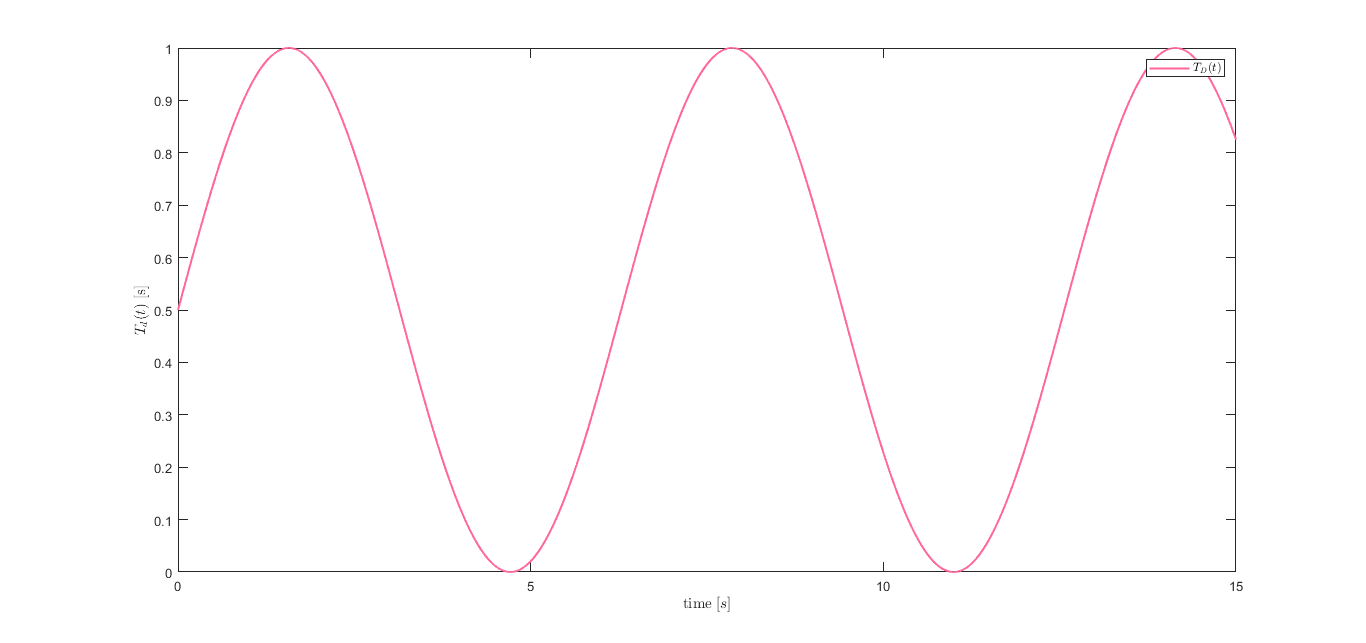
\includegraphics[width=1\linewidth]{Chapters/Chapter3/Figures/Sim1Fig1.png}
    \caption[Σενάριο Καθυστέρησης που ικανοποιεί τις Υποθέσεις]{Σενάριο Καθυστέρησης που ικανοποιεί τις Υποθέσεις}
    \label{Sim1Fig1}
\end{figure}

\begin{figure}[H]
    \centering
    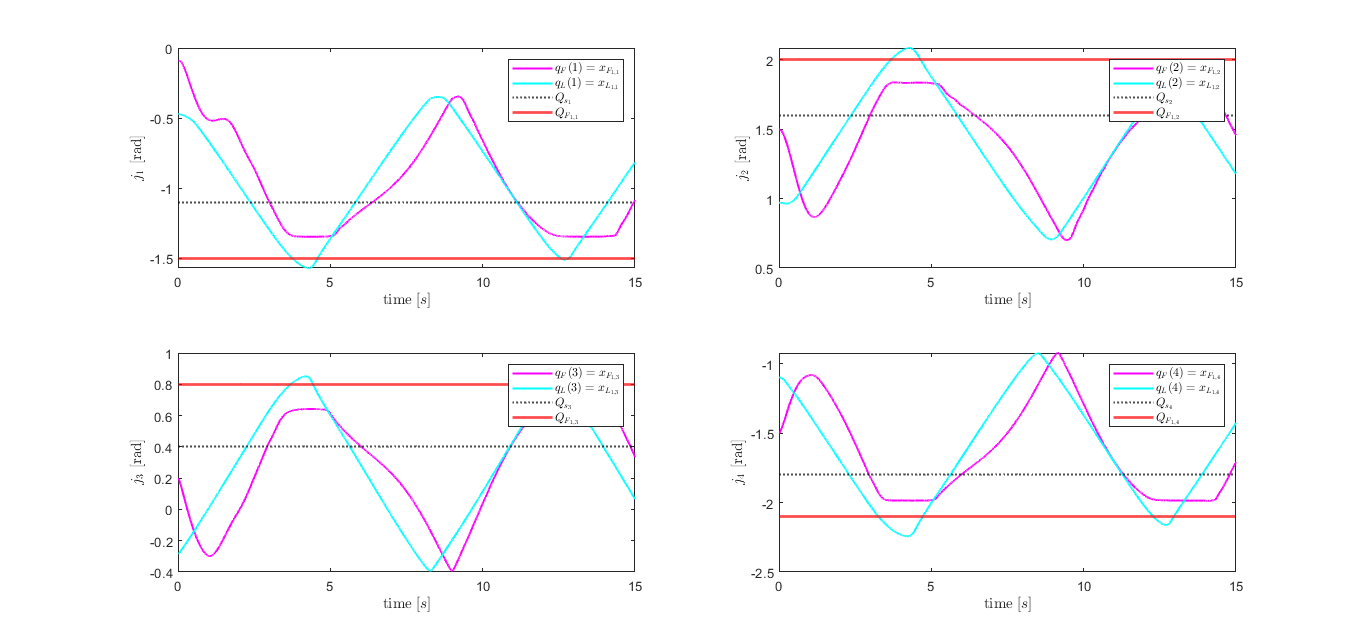
\includegraphics[width=1\linewidth]{Chapters/Chapter3/Figures/Sim1Fig2.png}
    \caption{Οι γωνίες των αρθρώσεων του \textit{Ακόλουθου} $x_{F_{1,i}}(t)$ μαζί με τις γωνίες των αρθρώσεων του \textit{Ηγέτη} $x_{L_{1,i}}(t)$.}
    \label{Sim1Fig2}
\end{figure}

\begin{figure}[H]
    \centering
    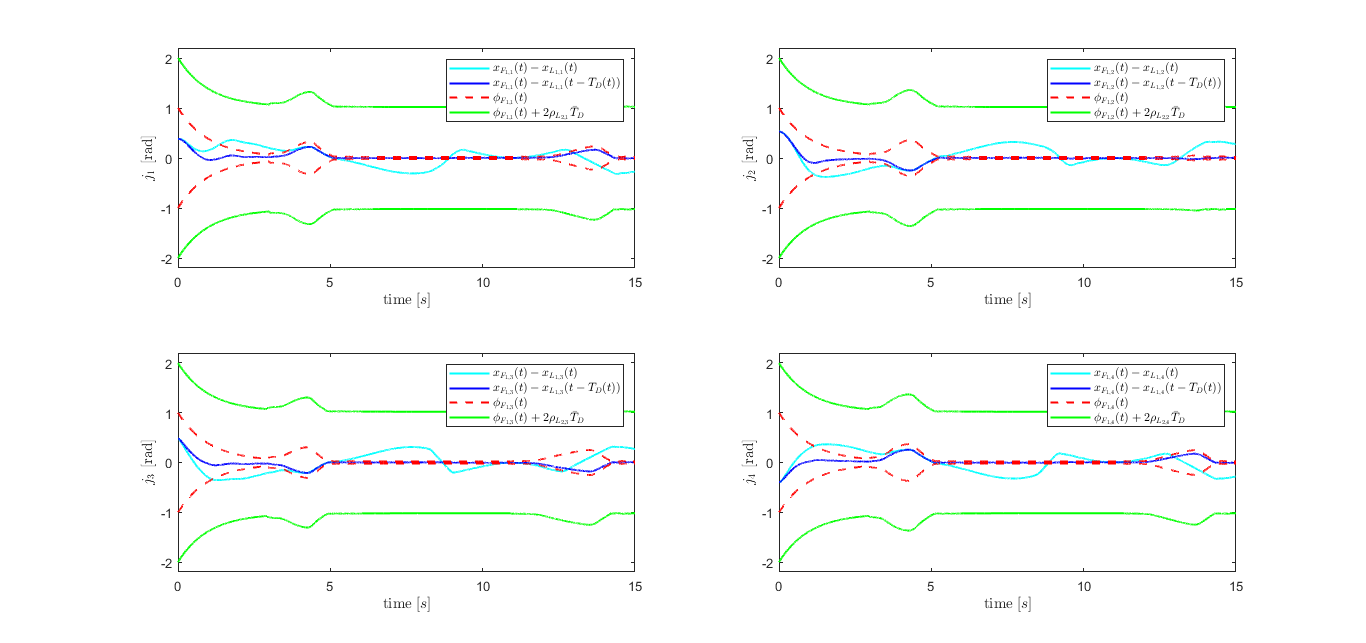
\includegraphics[width=1\linewidth]{Chapters/Chapter3/Figures/Sim1Fig3.png}
    \caption{Τα σφάλματα παρακολούθησης $x_{F_{1,i}}(t) - x_{L_{1,i}}(t - T_{D})$ και $x_{F_{1,i}}(t) - x_{L_{1,i}}(t)$ μαζί με τις αντίστοιχες συναρτήσεις επίδοσης $\phi_{F_{1,i}}(t)$.}
    \label{Sim1Fig3}
\end{figure}
\begin{figure}[!ht]
    \centering
    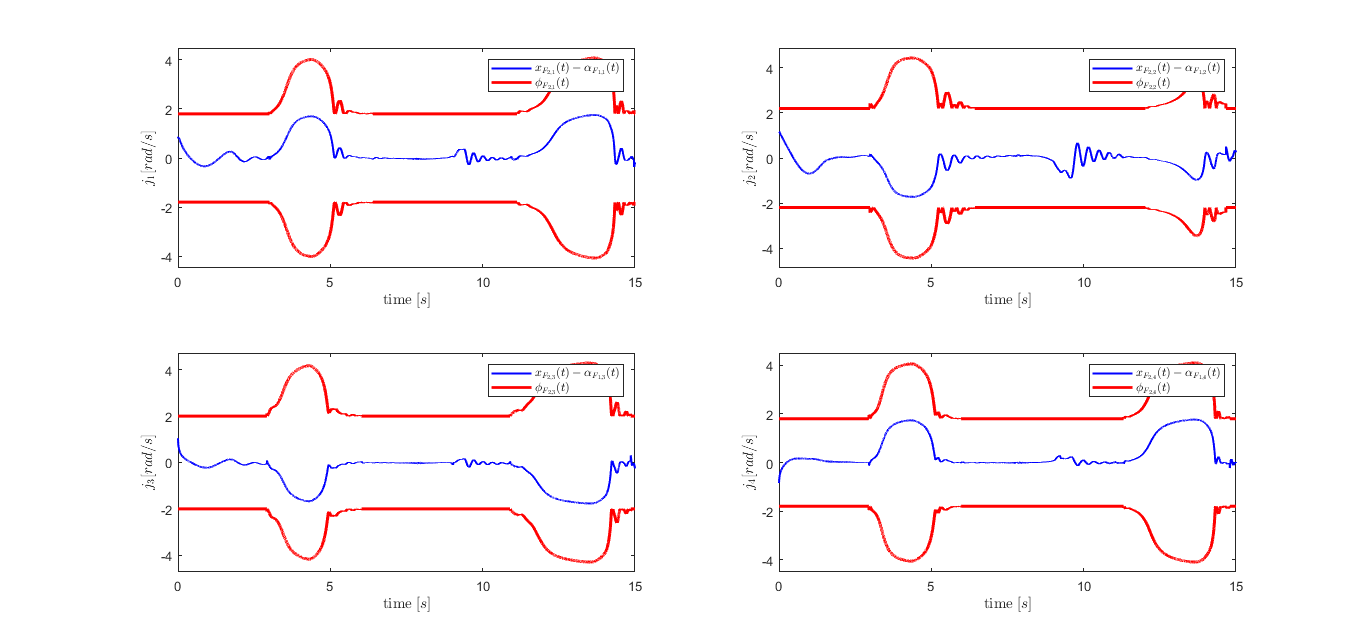
\includegraphics[width=1\linewidth]{Chapters/Chapter3/Figures/Sim1Fig4.png}
    \caption{Τα ενδιάμεσα σφάλματα $x_{F_{2,i}}(t) - \alpha_{F_{1,i}}(t)$ μαζί με τα αντίστοιχα όρια επίδοσης $\phi_{F_{2,i}}(t)$.}
    \label{Sim1Fig4}
\end{figure}

\begin{figure}[H]
    \centering
    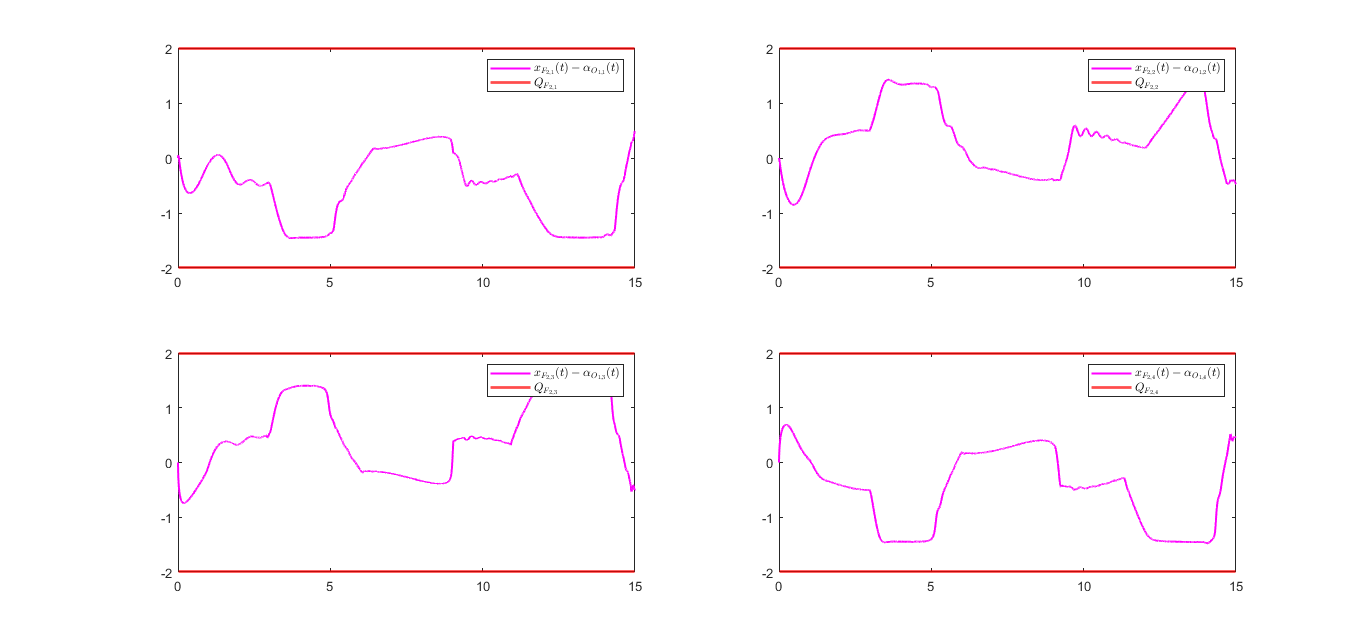
\includegraphics[width=1\linewidth]{Chapters/Chapter3/Figures/Sim1Fig5.png}
    \caption{Τα ενδιάμεσα σφάλματα $x_{F_{2,i}}(t) - \alpha_{O_{1,i}}(t)$ μαζί με τα αντίστοιχα όρια επίδοσης $Q_{F_{2,i}}$.}
    \label{Sim1Fig5}
\end{figure}



\begin{figure}[H]
    \centering
    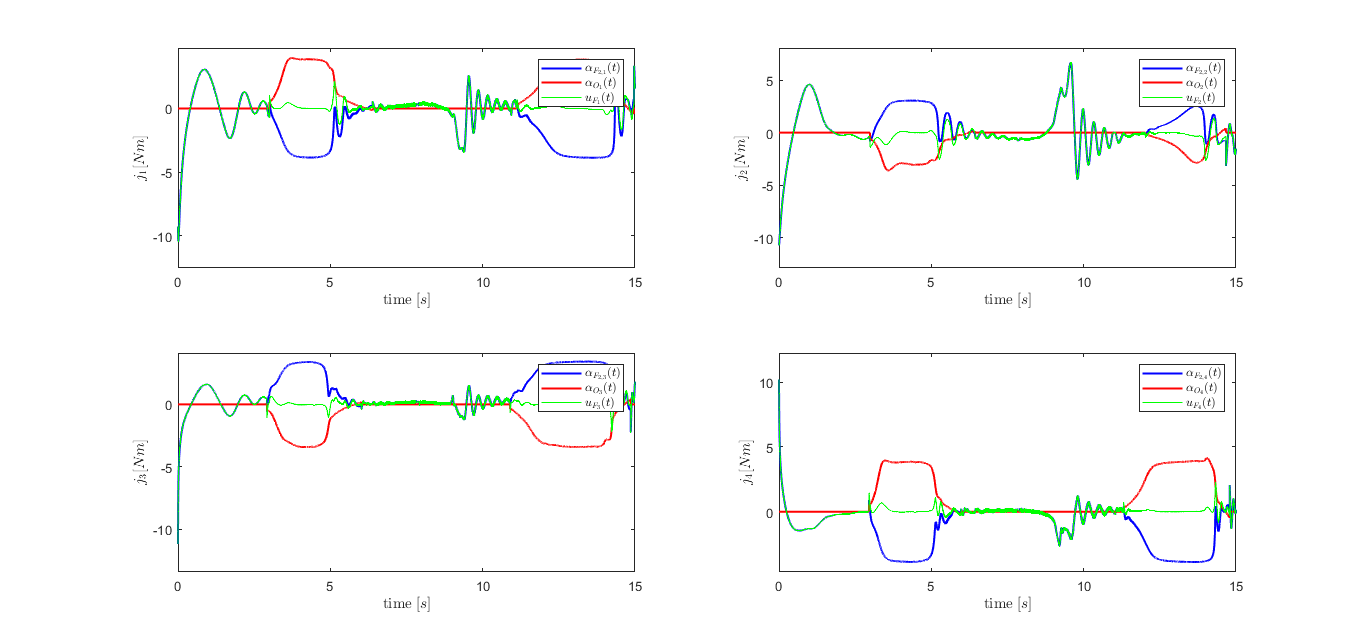
\includegraphics[width=1\linewidth]{Chapters/Chapter3/Figures/Sim1Fig6.png}
    \caption{Η είσοδος ελέγχου του Ακόλουθου $u_{F_{i}}(t)$.}
    \label{Sim1Fig6}
\end{figure}

\begin{figure}[H]
    \centering
    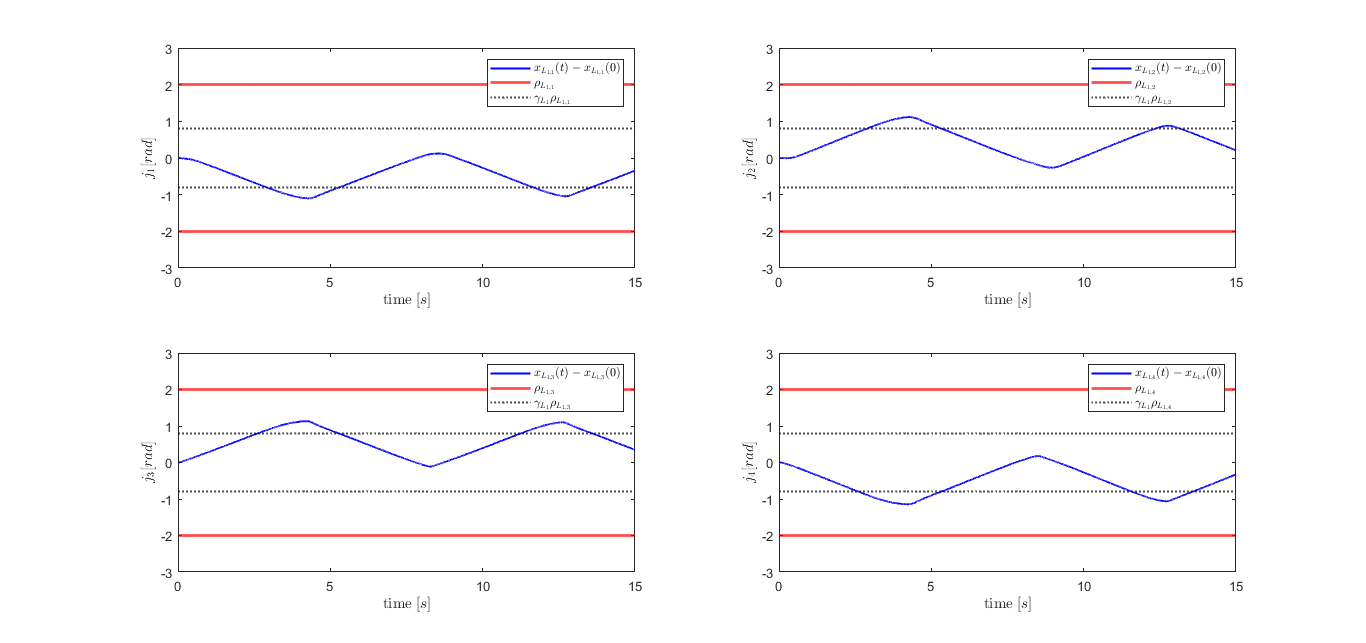
\includegraphics[width=1\linewidth]{Chapters/Chapter3/Figures/Sim1Fig7.png}
    \caption{Τα σφάλματα $x_{L_{1,i}}(t) - x_{L_{1,i}}(0)$ μαζί με τα αντίστοιχα όρια επίδοσης $\rho_{L_{1,i}}$.}
    \label{Sim1Fig7}
\end{figure}



\begin{figure}[H]
    \centering
    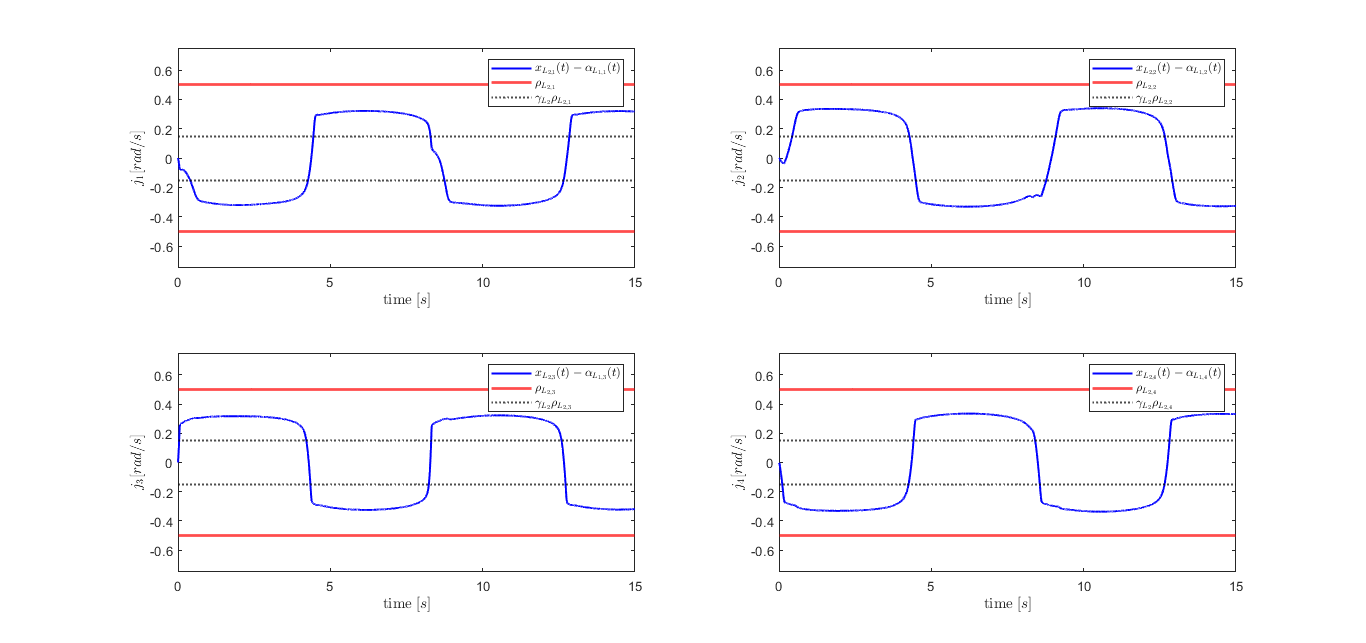
\includegraphics[width=1\linewidth]{Chapters/Chapter3/Figures/Sim1Fig8.png}
    \caption{Τα σφάλματα $x_{L_{2,i}}(t) - \alpha_{L_{1,i}}(t)$ μαζί με τα αντίστοιχα όρια επίδοσης $\rho_{L_{2,i}}$.}
    \label{Sim1Fig8}
\end{figure}

\begin{figure}[H]
    \centering
    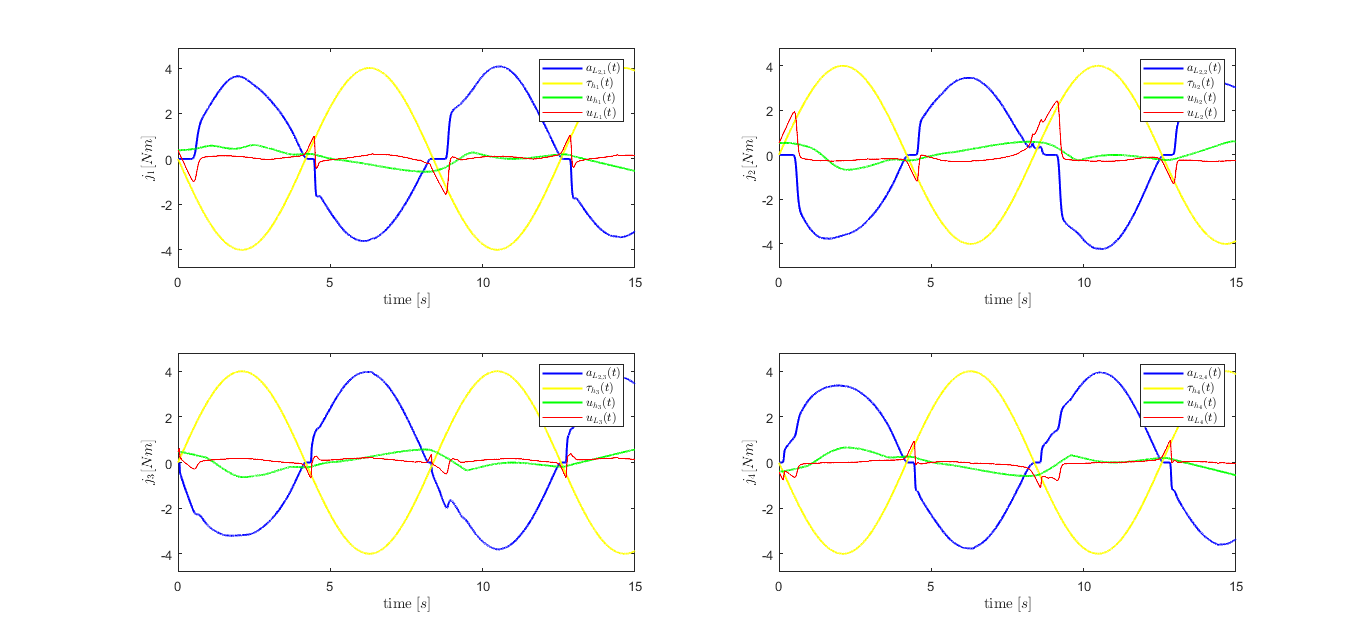
\includegraphics[width=1\linewidth]{Chapters/Chapter3/Figures/Sim1Fig9.png}
    \caption{Η είσοδος ελέγχου στον \textit{Ηγέτη} $u_{L_{i}}(t) = \alpha_{L_{2,i}}(t) + u_{H_{i}}(t)$ μαζί με τις δυνάμεις που ασκεί ο άνθρωπος πάνω του $\tau_{h_{i}}$.}
    \label{Sim1Fig9}
\end{figure}

\begin{observation}\label{fig:obs:1}
Στο σχήμα (\bref{Sim1Fig2}) βλέπουμε πως η ακριβής αναπαράσταση της καθυστερημένης τροχιάς του Ηγέτη στην \textbf{ΠΑΑ} με την παράλληλη αποφυγή του περιορισμού εξόδου στην \textbf{ΠΚΑ} με τρόπο αντίστοιχο με αυτό που απεικονίζεται στο Σχήμα~\bref{control_concept}, καταδεικνύει την επιτυχία του σχεδιαστικού ελέγχου στην αναδοχή προτεραιότητας στην συμπεριφορά του Ακόλουθου, έτσι ώστε να ακολουθεί πιστά τον Ηγέτη αλλά και να παραμένει ασφαλής όταν το πρώτο είναι αδύνατο.
\end{observation}

\bigskip
\begin{observation}\label{fig:obs:2}
Στο Σχήμα~\bref{Sim1Fig6} απεικονίζεται η είσοδος ελέγχου του Ακόλουθου. Όταν ο Ακόλουθος βρίσκεται στην Περιοχή Κινδύνου Ακόλουθου (ΠΚΑ), η είσοδος ελέγχου περιορίζεται, καθώς δίνεται προτεραιότητα στην ασφάλεια του συστήματος. Με την επιστροφή του Ακόλουθου στην Περιοχή Ασφαλείας Ακόλουθου (ΠΑΑ), και μετά από σύντομα μεταβατικά φαινόμενα, η είσοδος ελέγχου επανέρχεται, επιτρέποντας την αξιόπιστη αναπαράσταση της καθυστερημένης τροχιάς του Ηγέτη. Επιπλέον, στην Απόδειξη~\bref{proof_of_the:main} του Θεωρήματος~\bref{the:main} αποδείξαμε ότι η παρακολούθηση παραμένει φραγμένη καθόλη την διάρκεια του διμερούς τηλεχειρισμού, ενώ ο παράγοντας $u_{O}$ που προστέθηκε για την εξασφάλιση της ασφάλειας του Ακόλουθου, τείνει στο άπειρο όσο ο Ακόλουθος πλησιάζει τον περιορισμό $Q_{F_{1, i}}$.
\end{observation}

\bigskip
\begin{observation}\label{fig:obs:3}
Στα σχήματα (\bref{Sim1Fig3}) και (\bref{Sim1Fig4}) παρουσιάζονται τα σφάλματα παρακολούθησης γωνιών αλλά και ταχυτήτων, υπό τις τρέχουσες τροποποιημένες συναρτήσεις επίδοσης (\bref{phiF1_define}), (\bref{phiF2_define}), οι οποίες αυξάνουν τα όριά τους καθώς ο Ακόλουθος βρίσκεται εντός της \textbf{ΠΚΑ} για την διατήρηση της ευστάθειας. Αυτό έχει ως αποτέλεσμα την διατήρηση του Ελέγχου Προδιαγεγραμμένης Απόκρισης καθόλη την διάρκεια του ελέγχου.
\end{observation}

\bigskip
\begin{observation}\label{fig:obs:4}
Στα σχήματα (\bref{Sim1Fig7})-(\bref{Sim1Fig9}) παρουσιάζεται η συμπεριφορά του Ηγέτη, ανεπηρέαστη από την αλλαγή στρατηγικής από την πλευρά του Ακόλουθου εξαιτίας της χαμηλής απτικής ανάδρασης $u_{H}$(\bref{uH}). Με την αύξηση της τελευταίες, η δραστηριότητα του Ακόλουθου θα επιδρούσε στον Ηγέτη σε βαθμό που θα τον αποθάρρυνε από το να συνεχίσει την τροχιά του μακριά από την Περιοχή Ασφαλείας Ακόλουθου (ΠΑΑ).
\end{observation}

\section{Έλεγχος Ευρωστίας} \label{Chapter3Section3}
Καθώς η Υπόθεση~\bref{hyp:3} αποτελεί ικανή και όχι αναγκαία συνθήκη για την επίτευξη του στόχου ελέγχου και τίθεται κρίσιμο να εξεταστεί σε τι βαθμό καθίσταται αυτή περιοριστική, στα δύο επακόλουθα σενάρια θα μελετηθεί η ευρωστία του ελεγχόμενου συστήματος κλειστού βρόχου ως προς μεσαία και ακραία παραβίαση της υπόθεσης. Αυτό θα υλοποιηθεί με την σχεδίαση χρονική καθυστέρησης που $\dot{T}_D(t) > 1$. Από το έργο \cite{bresch2018robust}, φαίνεται εφικτή η διατήρηση της ευστάθειας, μάλλον και των στόχων ελέγχου, χωρίς καμία εγγύηση γι'αυτό.
Για την απόπειρα αυτή, καθίσταται σαφές η αύξηση του τελικού ορίου των συναρτήσεων επίδοσης $\rho^{\infty}_{F_{1,i}}$ από $\mathbf{0.02}$ σε $\mathbf{0.2}$ για όλες τις αρθρώσεις. Η πιο χαλαρή αυτή αντιμετώπιση του προβλήματος παρακολούθησης είναι ικανή να επιφέρει αποτελέσματα.

\bigskip
Στο σενάριο μέτριας παραβίασης θα χρησιμοποιηθεί η καθυστέρηση με άνω φράγμα $\bar{T}_{D} = 0.8\ \text{s}$.

\begin{figure}[H]
    \centering
    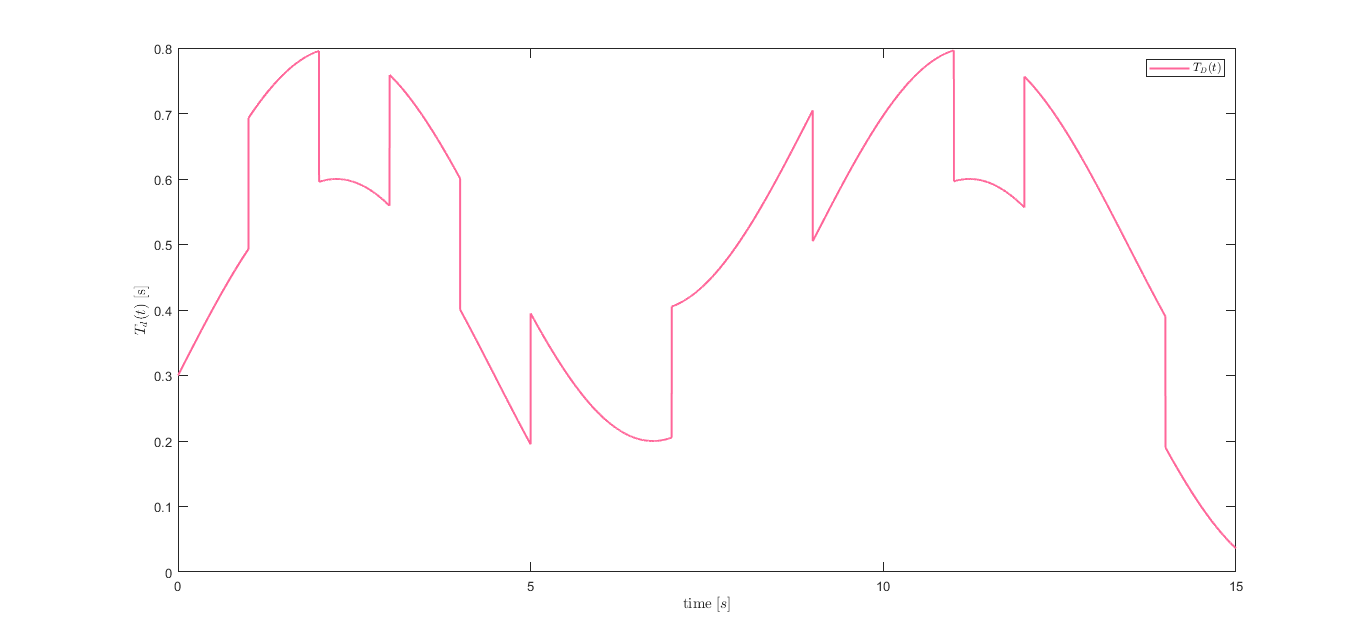
\includegraphics[width=1\linewidth]{Chapters/Chapter3/Figures/Sim2Fig1.png}
    \caption[Σενάριος μέτρια παραβίασης συνθηκών χρονικών καθυστερήσεων]{Σενάριο μέτριας παραβίασης συνθηκών χρονικών καθυστερήσεων}
    \label{Sim2Fig1}
\end{figure}

\begin{figure}[H]
    \centering
    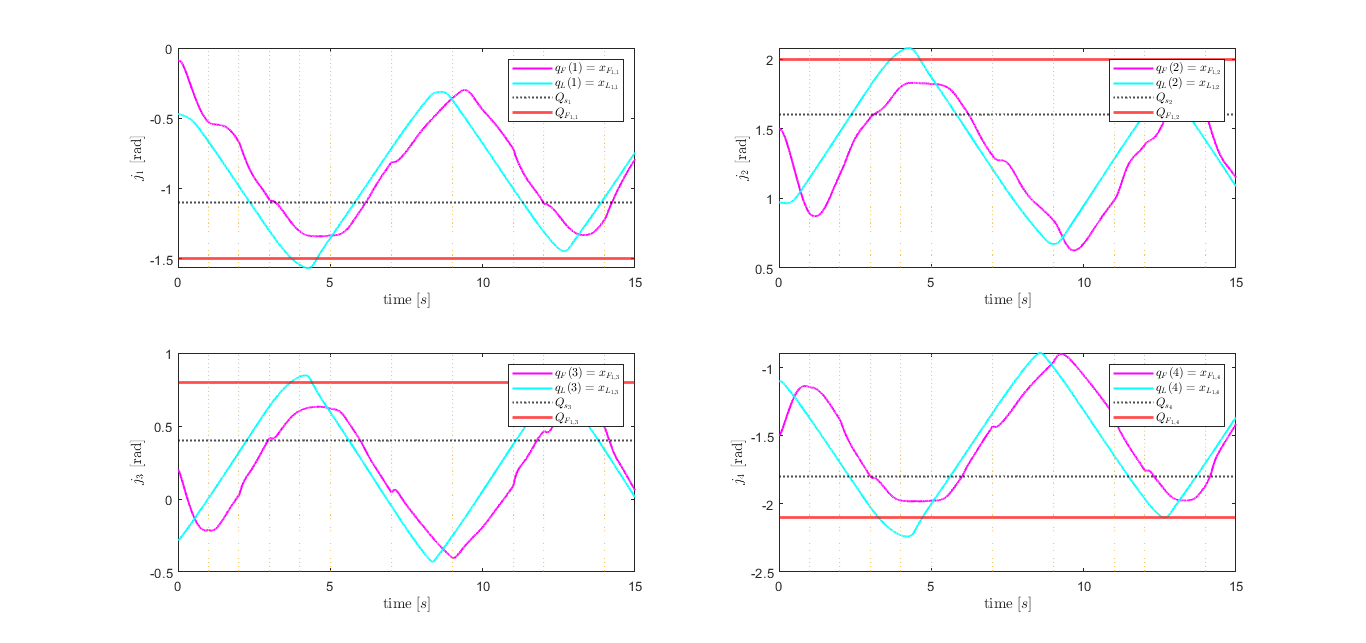
\includegraphics[width=1\linewidth]{Chapters/Chapter3/Figures/Sim2Fig2.png}
    \caption{Οι γωνίες των αρθρώσεων του \textit{Ακόλουθου} $x_{F_{1,i}}(t)$ μαζί με τις γωνίες των αρθρώσεων του \textit{Ηγέτη} $x_{L_{1,i}}(t)$.}
    \label{Sim2Fig2}
\end{figure}

\begin{figure}[H]
    \centering
    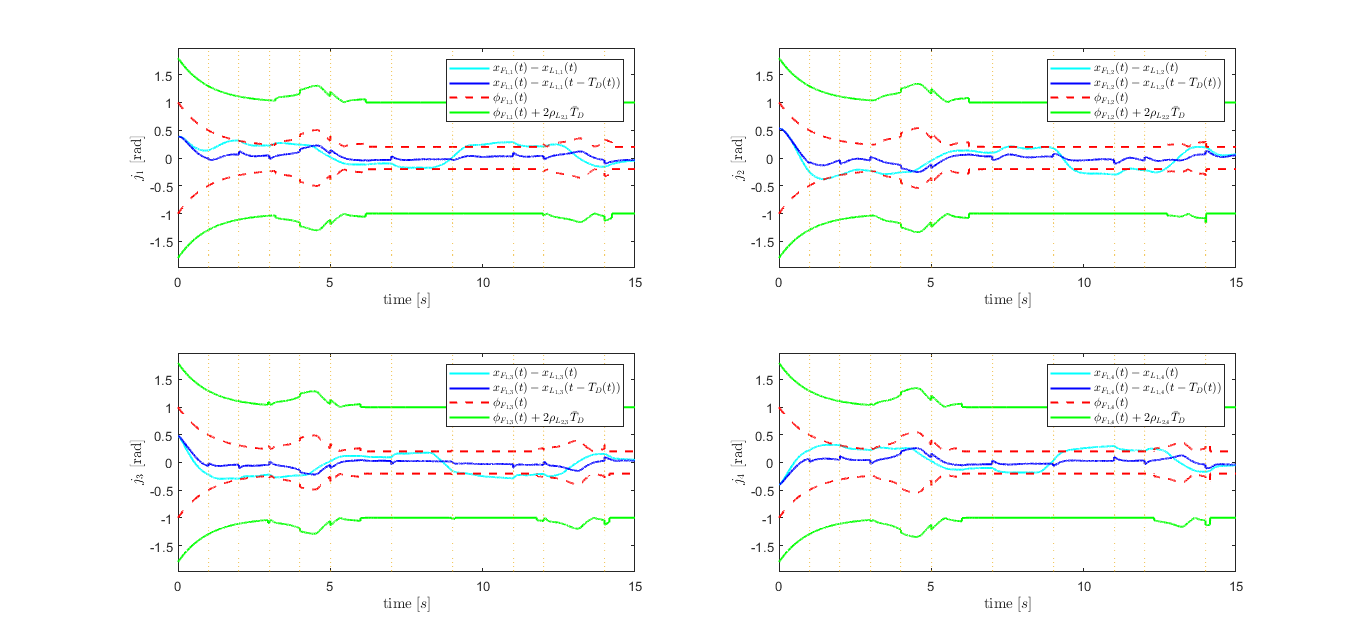
\includegraphics[width=1\linewidth]{Chapters/Chapter3/Figures/Sim2Fig3.png}
    \caption{Τα σφάλματα παρακολούθησης $x_{F_{1,i}}(t) - x_{L_{1,i}}(t - T_{D})$ και $x_{F_{1,i}}(t) - x_{L_{1,i}}(t)$ μαζί με τις αντίστοιχες συναρτήσεις επίδοσης $\phi_{F_{1,i}}(t)$.}
    \label{Sim2Fig3}
\end{figure}

\begin{figure}[H]
    \centering
    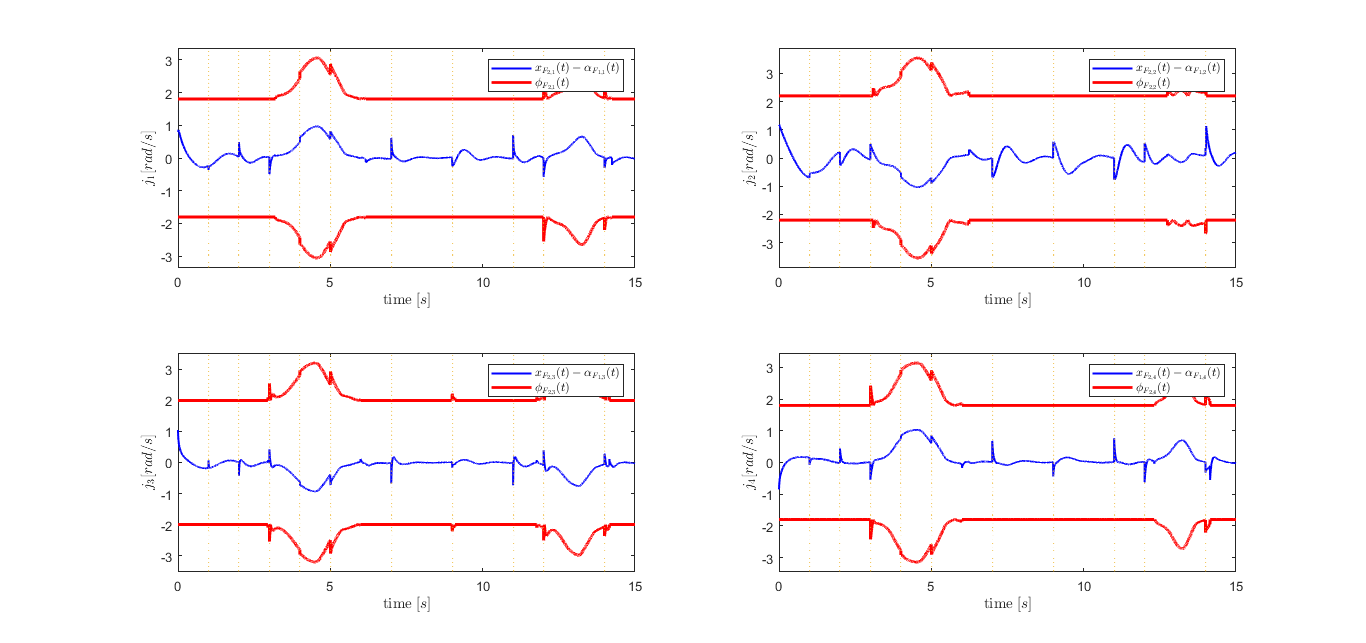
\includegraphics[width=1\linewidth]{Chapters/Chapter3/Figures/Sim2Fig4.png}
    \caption{Τα ενδιάμεσα σφάλματα $x_{F_{2,i}}(t) - \alpha_{F_{1,i}}(t)$ μαζί με τα αντίστοιχα όρια επίδοσης $\phi_{F_{2,i}}(t)$.}
    \label{Sim2Fig4}
\end{figure}

\begin{figure}[H]
    \centering
    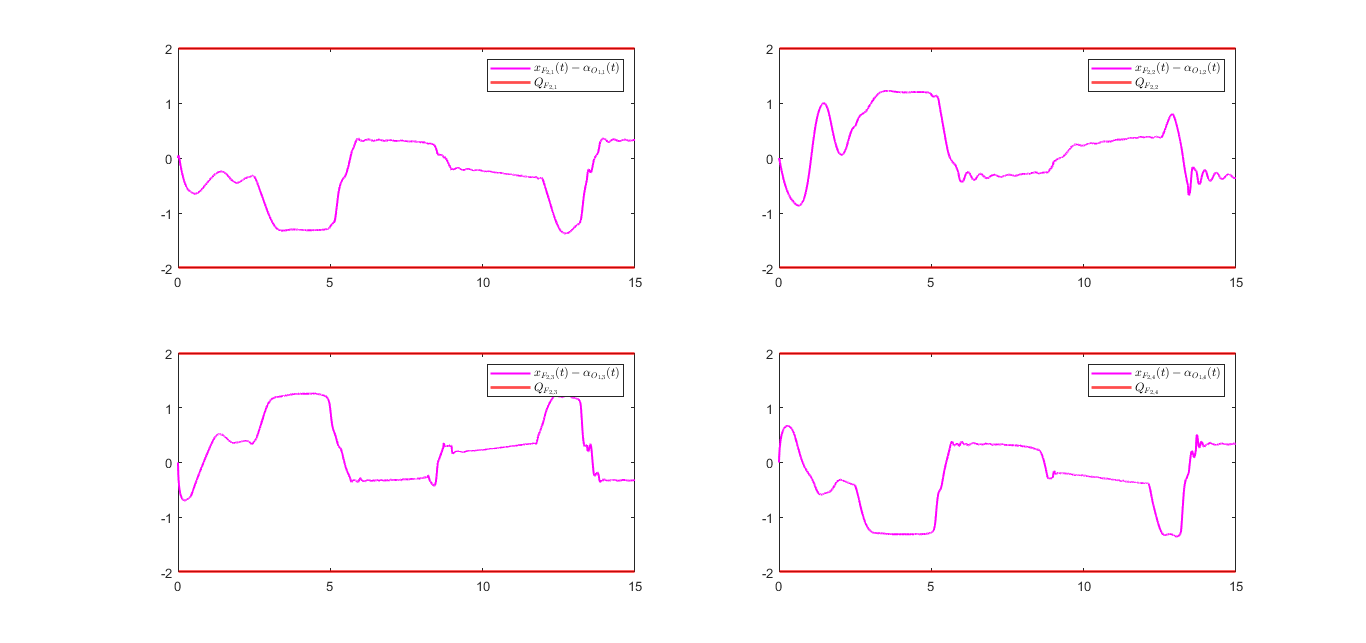
\includegraphics[width=1\linewidth]{Chapters/Chapter3/Figures/Sim2Fig5.png}
    \caption{Τα ενδιάμεσα σφάλματα $x_{F_{2,i}}(t) - \alpha_{O_{1,i}}(t)$ μαζί με τα αντίστοιχα όρια επίδοσης $Q_{F_{2,i}}$.}
    \label{Sim2Fig5}
\end{figure}



\begin{figure}[H]
    \centering
    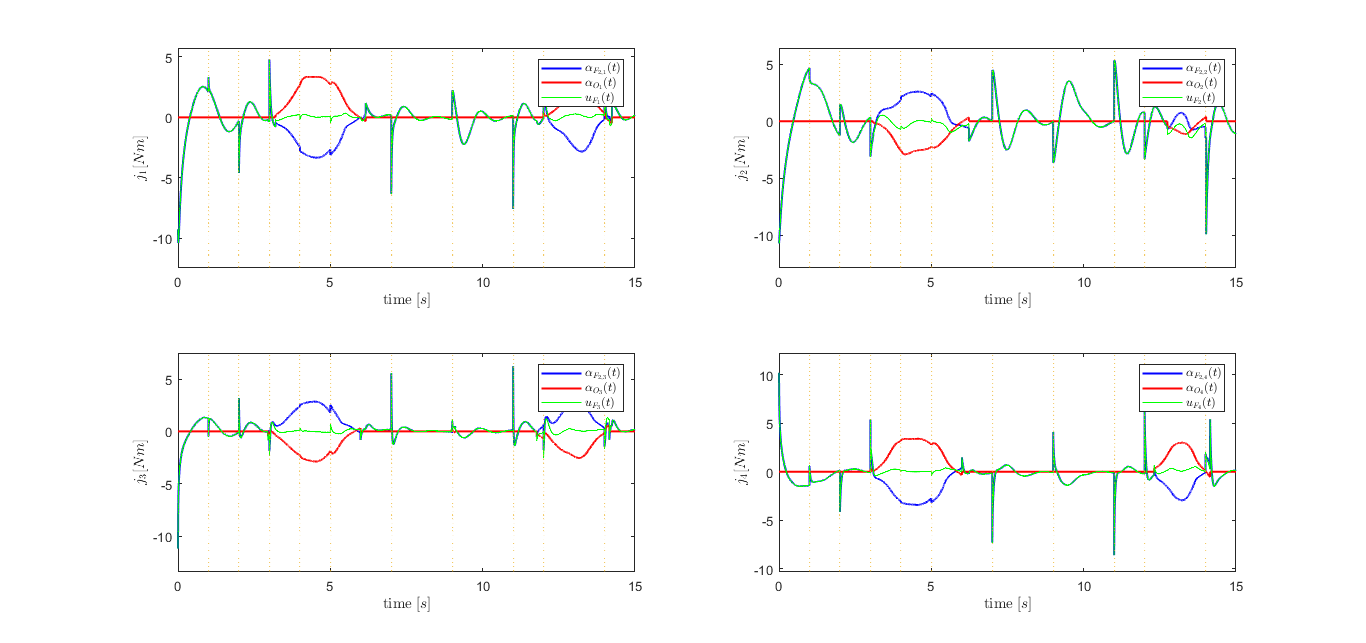
\includegraphics[width=1\linewidth]{Chapters/Chapter3/Figures/Sim2Fig6.png}
    \caption{Η είσοδος ελέγχου του \textit{Ακόλουθου} $u_{F_{i}}(t)$.}
    \label{Sim2Fig6}
\end{figure}

\begin{figure}[H]
    \centering
    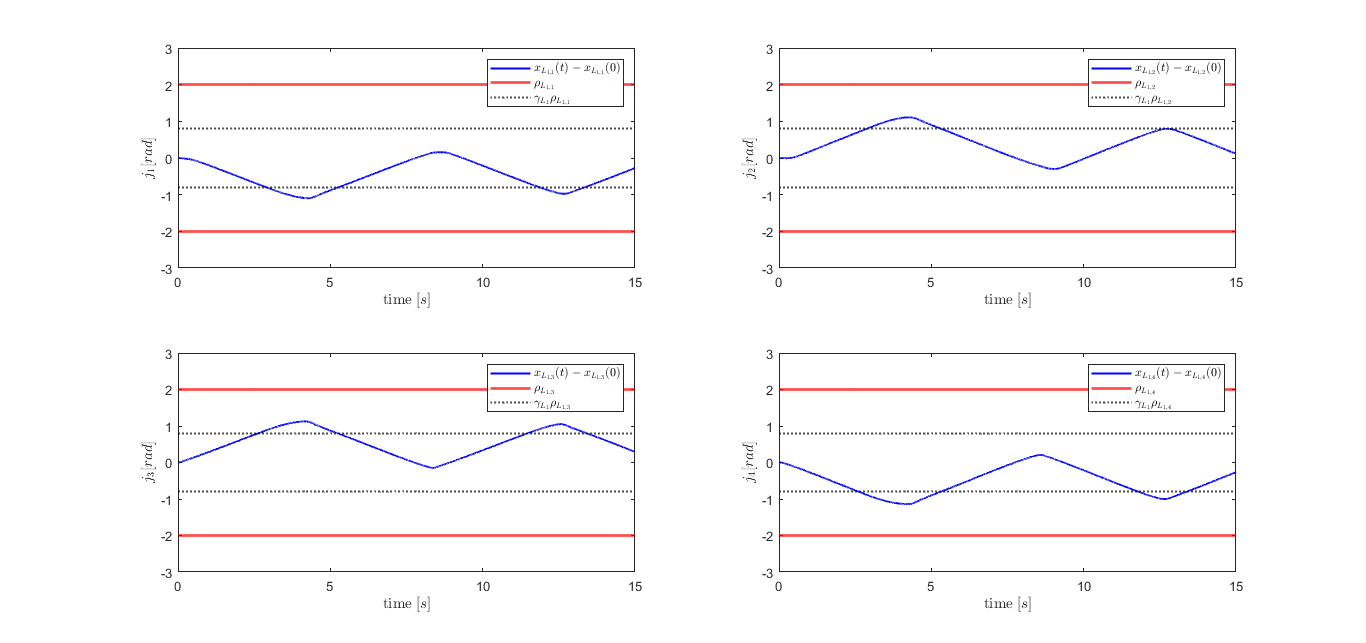
\includegraphics[width=1\linewidth]{Chapters/Chapter3/Figures/Sim2Fig7.png}
    \caption{Τα σφάλματα $x_{L_{1,i}}(t) - x_{L_{1,i}}(0)$ μαζί με τα αντίστοιχα όρια επίδοσης $\rho_{L_{1,i}}$.}
    \label{Sim2Fig7}
\end{figure}



\begin{figure}[H]
    \centering
    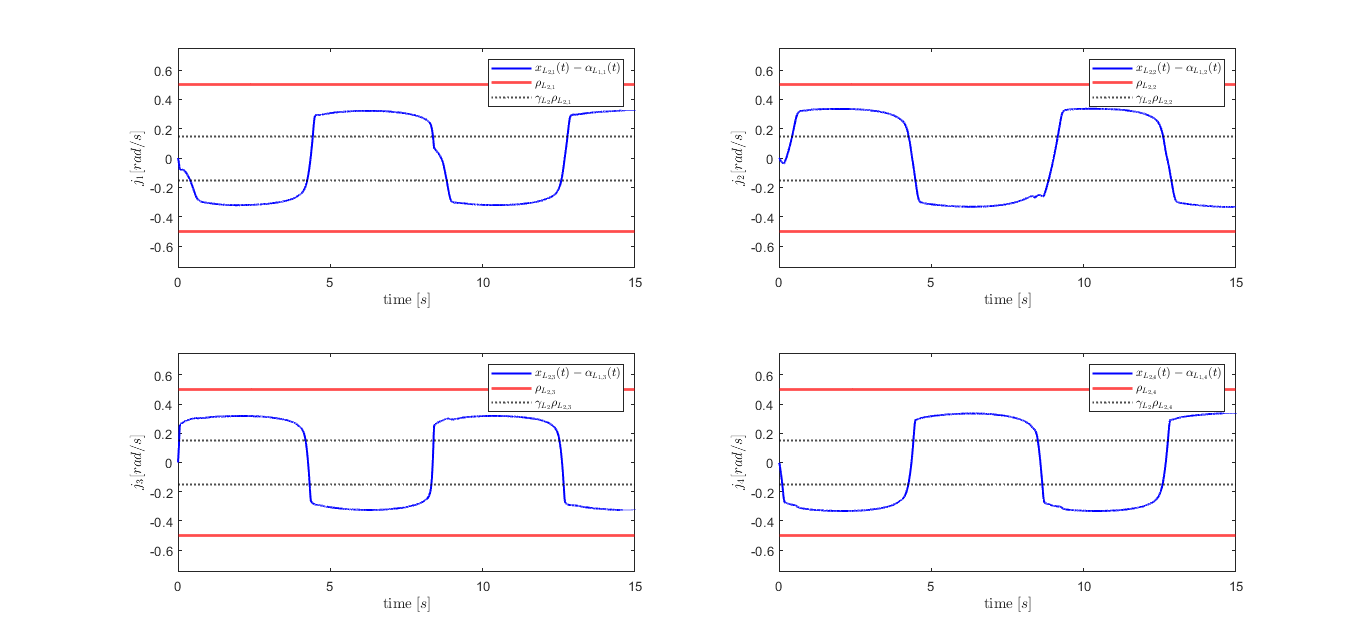
\includegraphics[width=1\linewidth]{Chapters/Chapter3/Figures/Sim2Fig8.png}
    \caption{Τα σφάλματα $x_{L_{2,i}}(t) - \alpha_{L_{1,i}}(t)$ μαζί με τα αντίστοιχα όρια επίδοσης $\rho_{L_{2,i}}$.}
    \label{Sim2Fig8}
\end{figure}

\begin{figure}[H]
    \centering
    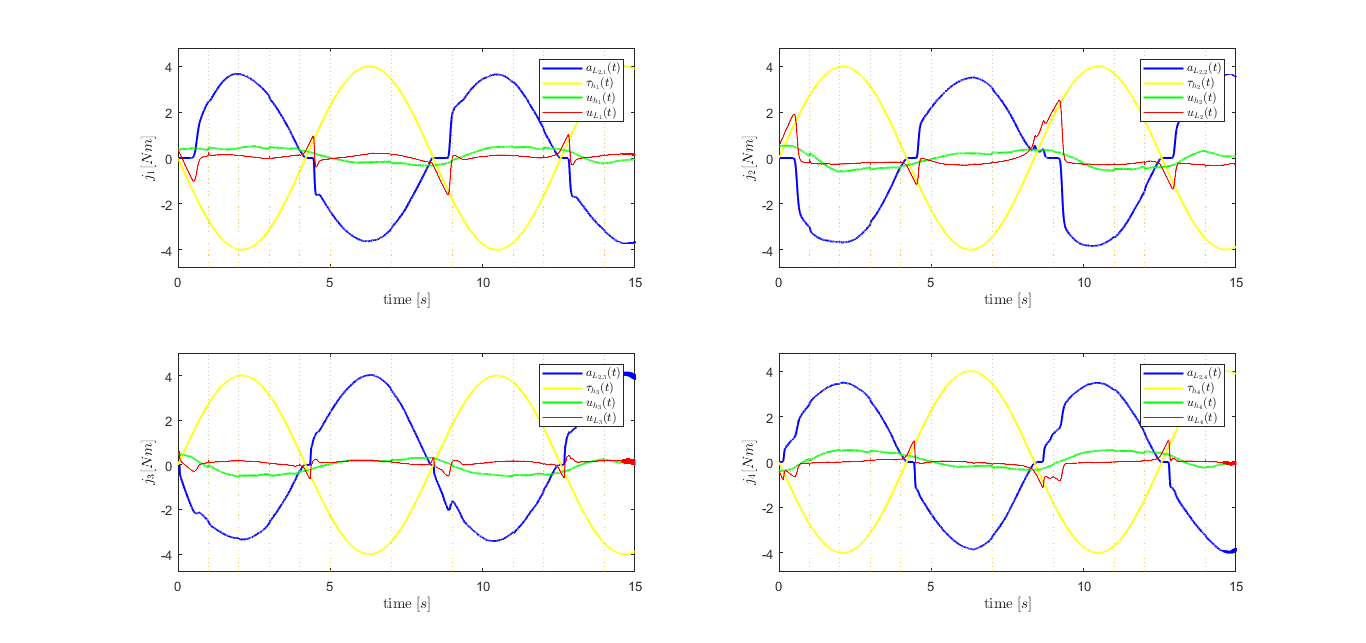
\includegraphics[width=1\linewidth]{Chapters/Chapter3/Figures/Sim2Fig9.png}
    \caption{Η είσοδος ελέγχου στον \textit{Ηγέτη} $u_{L_{i}}(t) = \alpha_{L_{2,i}}(t) + u_{H_{i}}(t)$ μαζί με τις δυνάμεις που ασκεί ο άνθρωπος πάνω του $\tau_{h_{i}}$.}
    \label{Sim2Fig9}
\end{figure}

\begin{observation} \label{figobs5}
Από τα σχήματα (\bref{Sim2Fig2}) και (\bref{Sim2Fig3}) φανερώτεται η ευρωστία του σχεδιαστικού ελέγχου παρόλι την παραβίασης της Υπόθεσης~\bref{hyp:3}. Η παρακολούθηση, αν και όχι ιδιαίτερα αυστηρή, επιτυγχάνεται, ενώ ταυτόχρονα ο Ακόλουθος διατηρείται ακέραιος, μένοντας σε απόσταση ασφαλείας από τους περιορισμούς κατάστασης εξόδου που τον οδηγουσέ ο Ηγέτης. Η επίδραση του φαινομένου αυτού είναι μηδανιμή στην συμπεριφορά του Ηγέτη (\bref{Sim2Fig7})-(\bref{Sim2Fig9}).
\end{observation}

\begin{observation} \label{figobs6}
Στο Σχήμα~\bref{Sim2Fig6}, παρατηρούνται σημαντικές αιχμές στην τιμή της εισόδου ελέγχου του Ακόλουθου κατά τις χρονικές στιγμές όπου η παράγωγος της χρονικής καθυστέρησης τείνει στο άπειρο. Ωστόσο, αυτές οι αιχμές εμφανίζονται μόνο στην Περιοχή Ασφαλείας Ακόλουθου (ΠΑΑ), όπου εφαρμόζεται η στρατηγική παρακολούθησης, και όχι στην Περιοχή Κινδύνου Ακόλουθου (ΠΚΑ). Αυτό υποδηλώνει ότι το καθεστώς ασφαλείας στην ΠΚΑ αποσβένει σημαντικές διακυμάνσεις στην είσοδο ελέγχου, αποτρέποντας τον Ακόλουθο από το να παραβεί τους περιορισμούς.
\end{observation}

\bigskip
Στο σενάριο ακραίας παραβίασης θα χρησιμοποιηθεί η καθυστέρηση με άνω φράγμα $\bar{T}_{D} = 0.3\ \text{s}$. Ύστερα από πολλαπλές δοκιμές, η ελάχιστη τιμή του φράγματος της συνάρτησης επίδοσης στην τελική κατάσταση (\bref{rhoinfty}) που παρέχει ευστάθεια στο ελεγχόμενο σύστημα ήταν από $\mathbf{0.2}$ σε $\mathbf{0.25}$ για κάθε άρθρωση.


\begin{figure}[H]
    \centering
    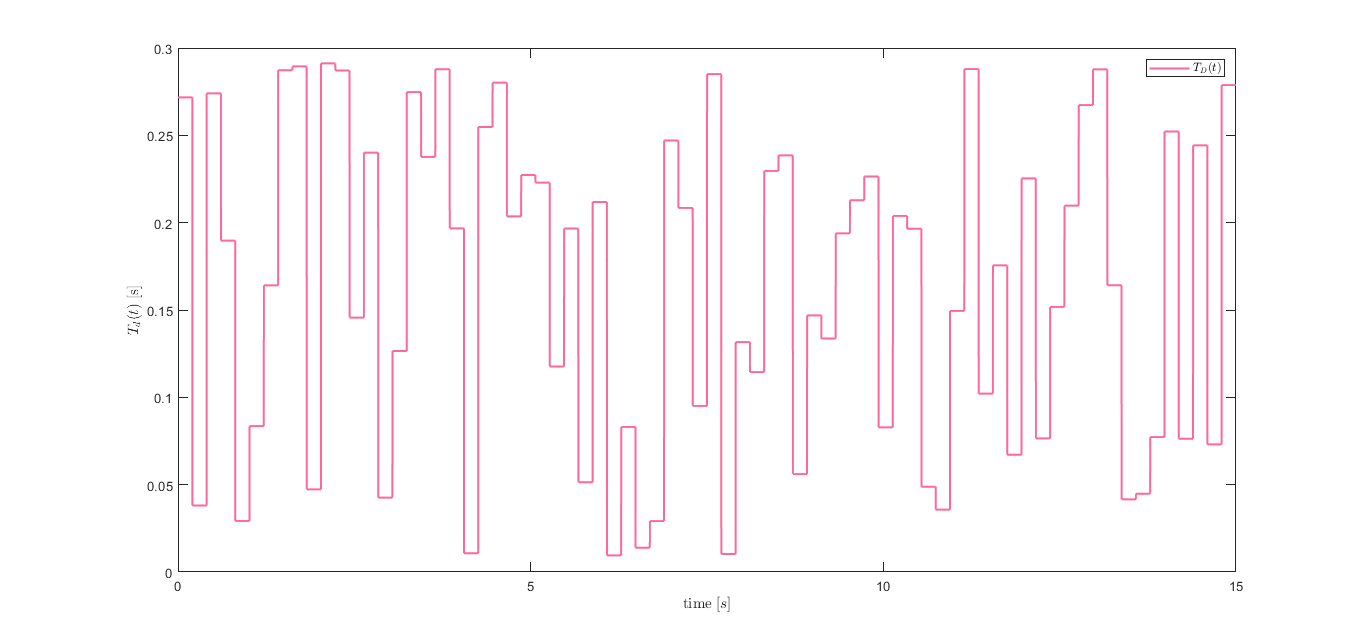
\includegraphics[width=0.9\linewidth]{Chapters/Chapter3/Figures/Sim3Fig1.png}
    \caption[Σενάριο ακραίας παραβίασης συνθηκών χρονικών καθυστερήσεων]{Σενάριο ακραίας παραβίασης συνθηκών χρονικών καθυστερήσεων}
    \label{Sim3Fig1}
\end{figure}

\begin{figure}[H]
    \centering
    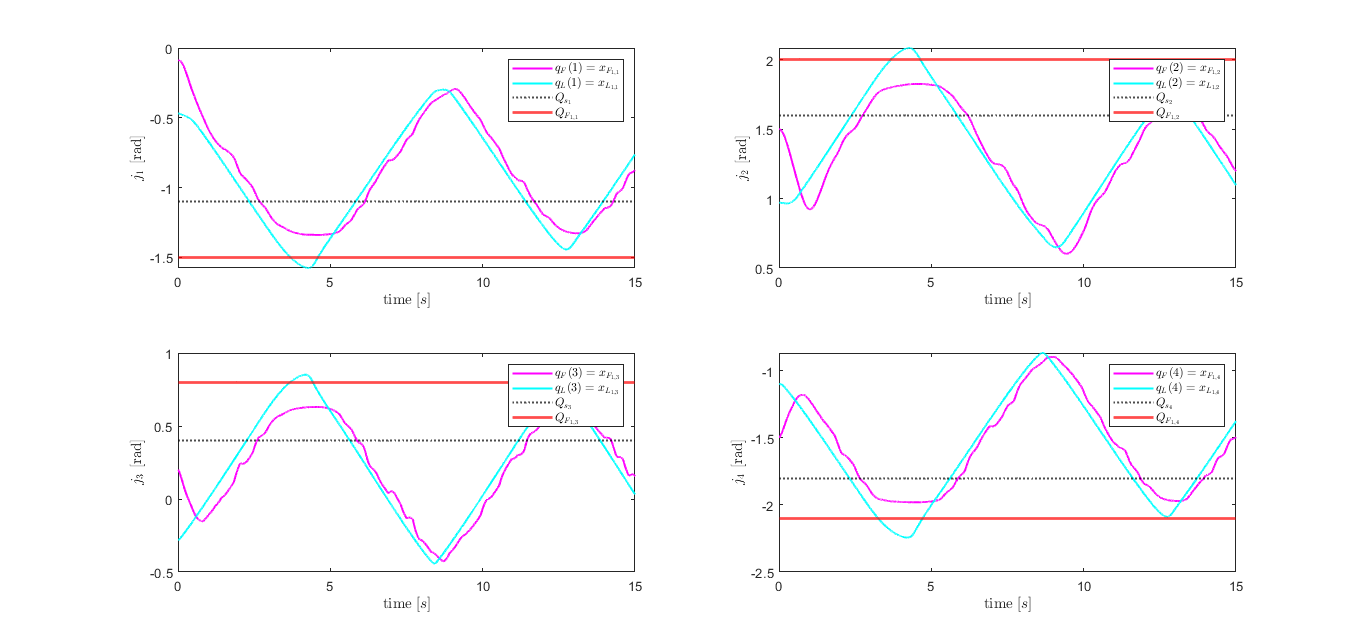
\includegraphics[width=1\linewidth]{Chapters/Chapter3/Figures/Sim3Fig2.png}
    \caption{Οι γωνίες των αρθρώσεων του \textit{Ακόλουθου} $x_{F_{1,i}}(t)$ μαζί με τις γωνίες των αρθρώσεων του \textit{Ηγέτη} $x_{L_{1,i}}(t)$.}
    \label{Sim3Fig2}
\end{figure}

\begin{figure}[H]
    \centering
    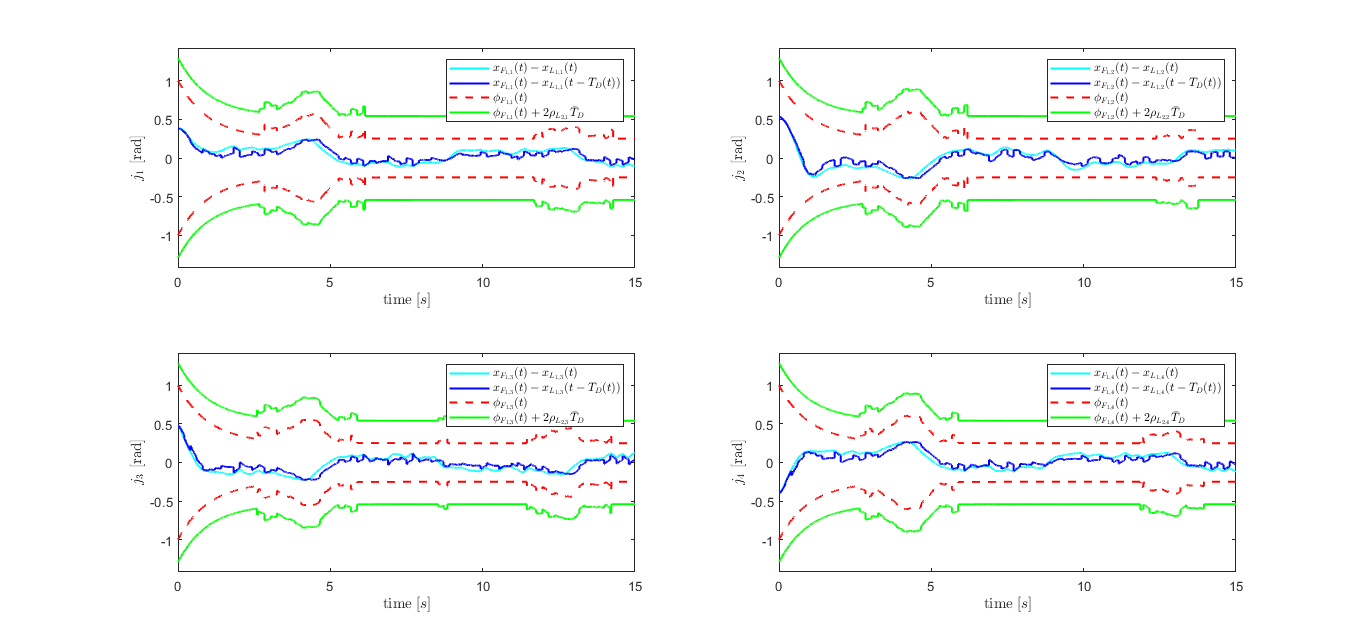
\includegraphics[width=1\linewidth]{Chapters/Chapter3/Figures/Sim3Fig3.png}
    \caption{Τα σφάλματα παρακολούθησης $x_{F_{1,i}}(t) - x_{L_{1,i}}(t - T_{D})$ και $x_{F_{1,i}}(t) - x_{L_{1,i}}(t)$ μαζί με τις αντίστοιχες συναρτήσεις επίδοσης $\phi_{F_{1,i}}(t)$.}
    \label{Sim3Fig3}
\end{figure}

\begin{figure}[H]
    \centering
    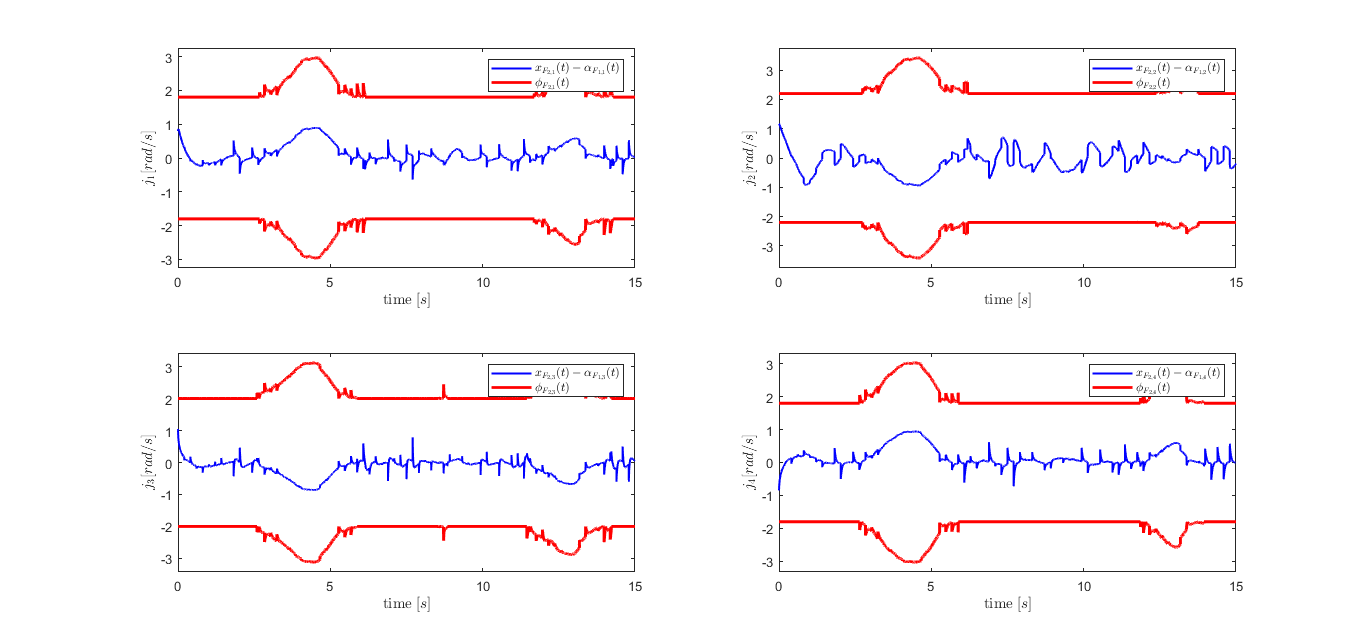
\includegraphics[width=1\linewidth]{Chapters/Chapter3/Figures/Sim3Fig4.png}
    \caption{Τα ενδιάμεσα σφάλματα $x_{F_{2,i}}(t) - \alpha_{F_{1,i}}(t)$ μαζί με τα αντίστοιχα όρια επίδοσης $\phi_{F_{2,i}}(t)$.}
    \label{Sim3Fig4}
\end{figure}

\begin{figure}[H]
    \centering
    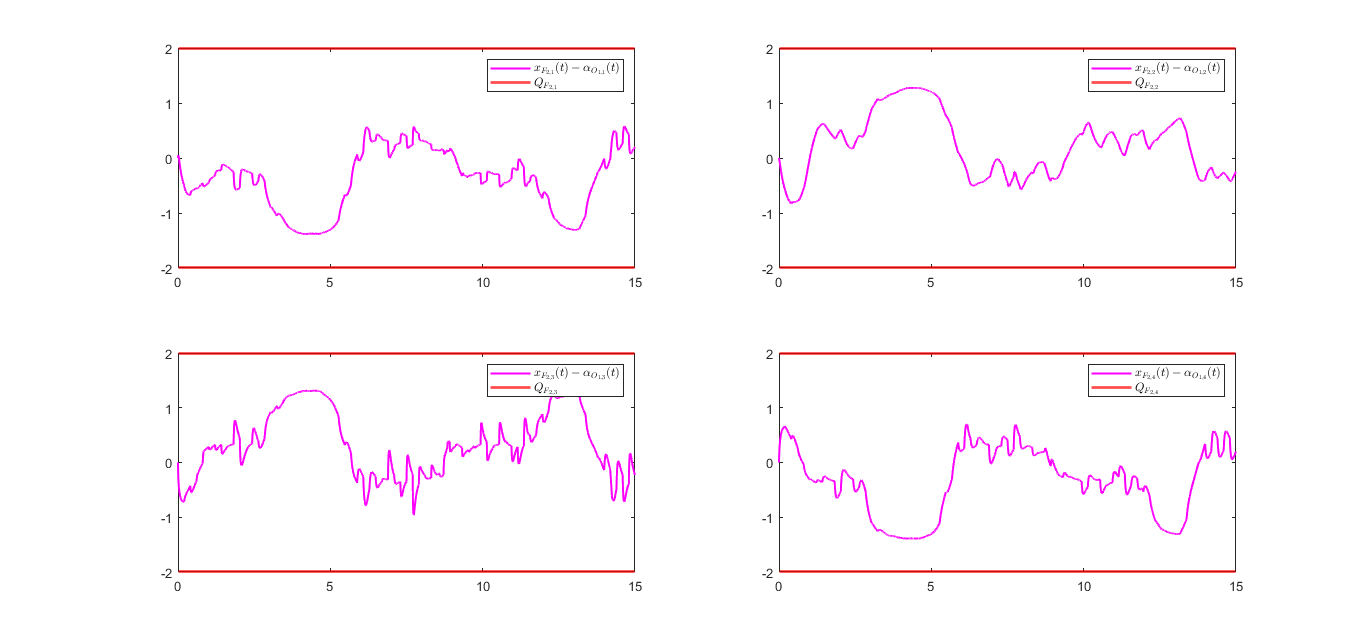
\includegraphics[width=1\linewidth]{Chapters/Chapter3/Figures/Sim3Fig5.png}
    \caption{Τα ενδιάμεσα σφάλματα $x_{F_{2,i}}(t) - \alpha_{O_{1,i}}(t)$ μαζί με τα αντίστοιχα όρια επίδοσης $Q_{F_{2,i}}$.}
    \label{Sim3Fig5}
\end{figure}



\begin{figure}[H]
    \centering
    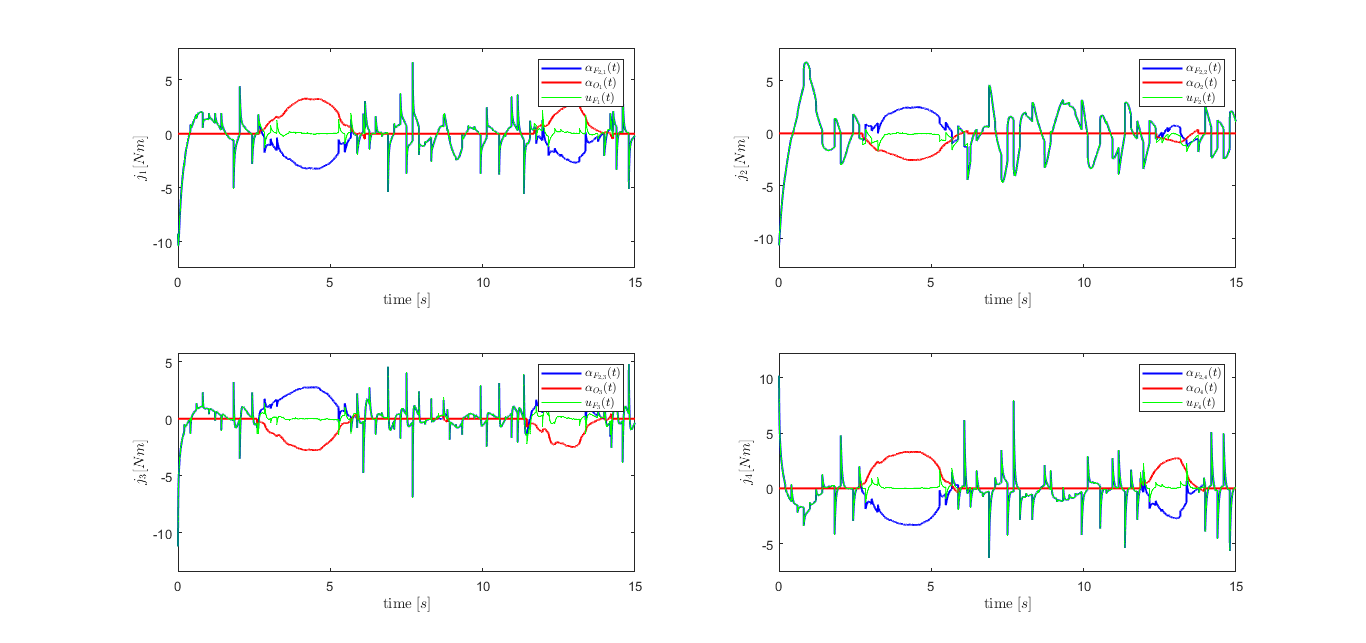
\includegraphics[width=1\linewidth]{Chapters/Chapter3/Figures/Sim3Fig6.png}
    \caption{Η είσοδος ελέγχου του \textit{Ακόλουθου} $u_{F_{i}}(t)$.}
    \label{Sim3Fig6}
\end{figure}

\begin{figure}[H]
    \centering
    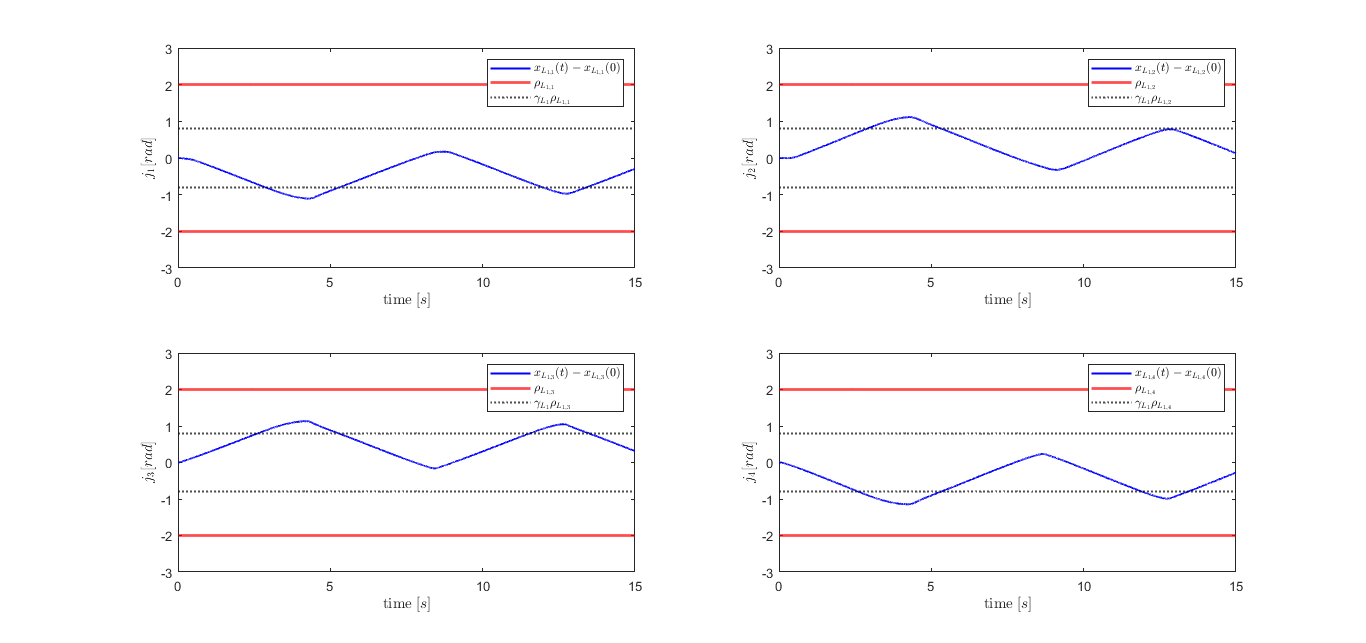
\includegraphics[width=1\linewidth]{Chapters/Chapter3/Figures/Sim3Fig7.png}
    \caption{Τα σφάλματα $x_{L_{1,i}}(t) - x_{L_{1,i}}(0)$ μαζί με τα αντίστοιχα όρια επίδοσης $\rho_{L_{1,i}}$.}
    \label{Sim3Fig7}
\end{figure}



\begin{figure}[H]
    \centering
    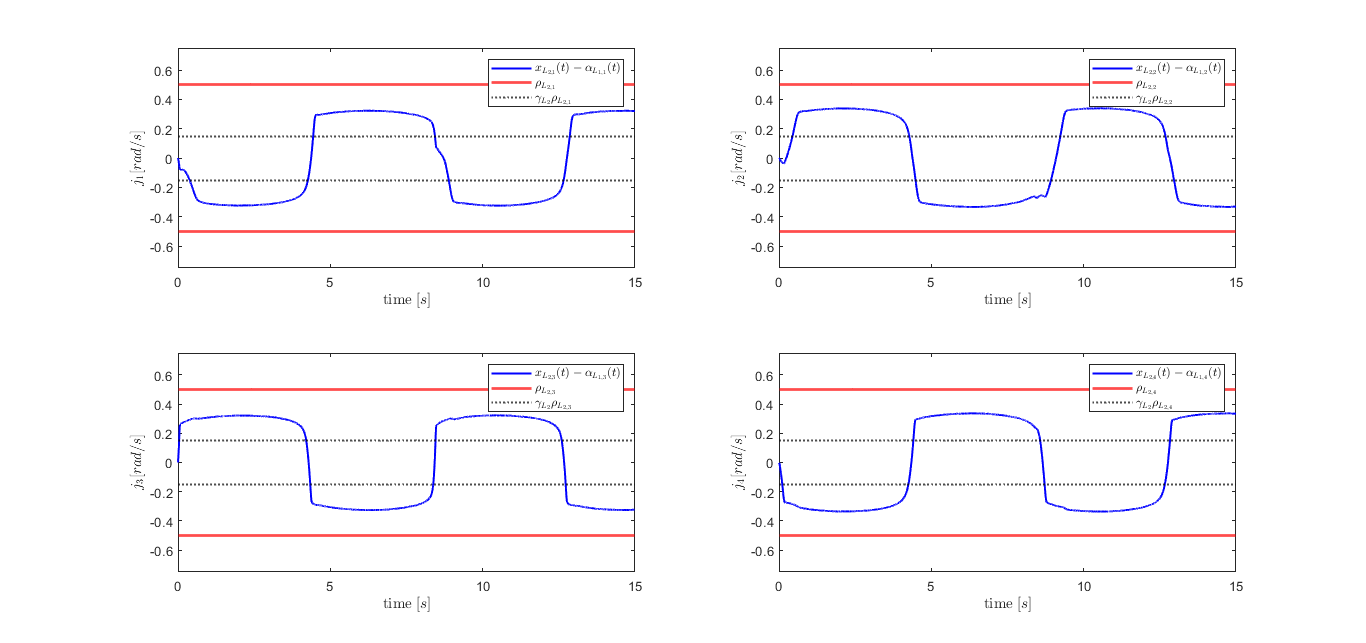
\includegraphics[width=1\linewidth]{Chapters/Chapter3/Figures/Sim3Fig8.png}
    \caption{Τα σφάλματα $x_{L_{2,i}}(t) - \alpha_{L_{1,i}}(t)$ μαζί με τα αντίστοιχα όρια επίδοσης $\rho_{L_{2,i}}$.}
    \label{Sim3Fig8}
\end{figure}

\begin{figure}[H]
    \centering
    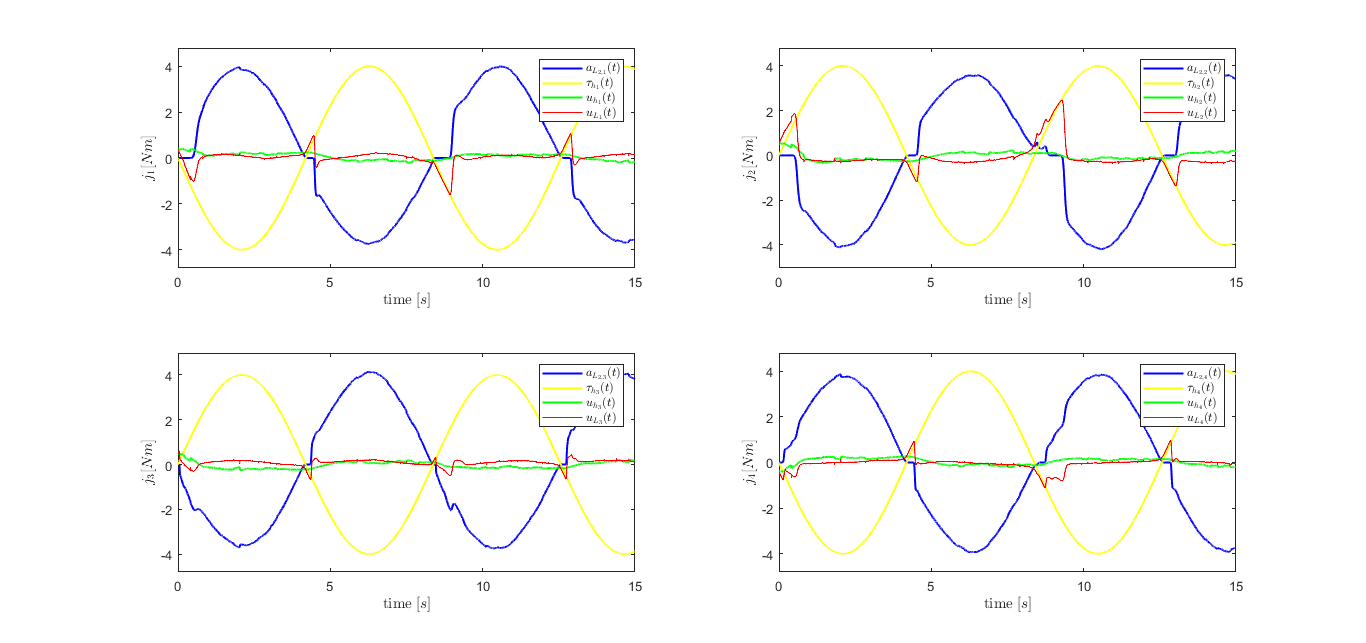
\includegraphics[width=1\linewidth]{Chapters/Chapter3/Figures/Sim3Fig9.png}
    \caption{Η είσοδος ελέγχου στον \textit{Ηγέτη} $u_{L_{i}}(t) = \alpha_{L_{2,i}}(t) + u_{H_{i}}(t)$ μαζί με τις δυνάμεις που ασκεί ο άνθρωπος πάνω του $\tau_{h_{i}}$.}
    \label{Sim3Fig9}
\end{figure}

\begin{observation} \label{figobs20} 
Από την ανάλυση όλων των σχημάτων που αφορούν τον έλεγχο του Ακόλουθου (Σχήματα~\bref{Sim3Fig2} έως~\bref{Sim3Fig6}), προκύπτει ότι, ακόμη και σε αυτή την ακραία περίπτωση, με χαμηλό άνω φράγμα στην χρονική καθυστέρηση και με σημαντική αύξηση της σχεδιαστικής παραμέτρου $\rho^{\infty}_{F_{1,i}}$, η ευρωστία και των δύο ρομποτικών συστημάτων διατηρείται, ενώ οι προδιαγεγραμμένοι στόχοι ελέγχου επιτυγχάνονται. 
\end{observation}

\begin{observation} \label{figobs21}
Στο Σχήμα~\bref{Sim3Fig6}, παρατηρούνται ακόμα πιο σημαντικές αιχμές στην τιμή της εισόδου ελέγχου του Ακόλουθου από τις αντίστοιχες στο Σενάριο~\bref{Chapter3Section3Subsection1}, οι οποίες επιφέρουν την ανάγκη της επιπλέον αύξησης του ορίου του σφάλματος εξόδου στην τελική κατάσταση. Παρόλα αυτά, και στο παρόν ακραίο σενάριο παραβίασης, εντός της Περιοχής Κινδύνου Ακόλουθου (ΠΚΑ), οι έντονες αυτές διακυμάνσεις εξουδετερώνονται σε βαθμό ικανοποιητικό που να μην παραβιάζονται οι περιορισμοί κατάστασης εξόδου.
\end{observation}

\let\cleardoublepage\clearpage
	\chapter{Επίλογος} \label{Chapter4}
Ανακεφαλαιώνοντας, στην παρούσα διπλωματική εργασία αντιμετωπίστηκε το πρόβλημα του διμερούς τηλεχειρισμού σε συστήματα ρομποτικών βραχιόνων τύπου Ηγέτη-Ακόλουθου με άγνωστες και χρονικά μεταβαλλόμενες καθυστερήσεις στο ψηφιακό κανάλι επικοινωνίας και περιορισμούς κατάστασης εξόδου στις αρθρώσεις του Ακόλουθου. Αναπτύχθηκε μια αρχιτεκτονική ελέγχου βασισμένη στον Έλεγχο Προκαθορισμένης Απόδοσης (PPC), που επιτρέπει δυναμική αλλαγή προτεραιοτήτων μεταξύ ακριβούς παρακολούθησης και ασφάλειας, επιλύοντας το ανταγωνιστικό δίλημμα μεταξύ αυτών των δύο στόχων. Η απόδοση του συστήματος αποδείχθηκε συνάρτηση των καθυστερήσεων: όσο μεγαλύτερες οι καθυστερήσεις, τόσο μεγαλύτερα τα εγγυημένα όρια σφάλματος παρακολούθησης, με υποβάθμιση της απόδοσης σε ακραίες περιπτώσεις. Η μαθηματική θεμελίωση του ελέγχου τεκμηριώθηκε πλήρως, και οι εκτενείς προσομοιώσεις σε ρεαλιστικά μοντέλα επιβεβαίωσαν την αποτελεσματική διαχείριση των καθυστερήσεων και την αποφυγή επικίνδυνων ζωνών από τον Ακόλουθο, διατηρώντας την ευστάθεια, την απόδοση και την ασφάλεια του συστήματος, ακόμη και όταν οι καθυστερήσεις υπερέβαιναν τα καθορισμένα όρια.

\bigskip
Παρά τη σημαντική πρόοδο που επιτεύχθηκε, υπάρχουν ακόμα περιθώρια βελτίωσης στο σχεδιασμό ελέγχου για τη διαχείριση πιο πολύπλοκων και δυναμικών περιβαλλόντων. Μελλοντικές μελέτες μπορούν να επεκταθούν από τον χώρο των γωνιών στον κατερσιανό XYZ χώρο, ενώ η απαίτηση για όσο το δυνατόν λιγότερη γνώση αναφορικά με τις διάφοες κλάσεις μη-γραμμικών συστημάτων αποτελεί μείζον θέμα διερεύνησης. Επιπλέον, θα μπορούσαν θα μελετηθούν σενάρια ασυνεχούς και/ή χωρίς γνώση άνω φράγματος χρονικών καθυστερήσεων, περιπτώσεις που μελετήθηκαν στον έλεγχο ευρωστίας αλλά δεν εγγυήθηκε η επιτυχής και μαθηματικά αποδεδειγμένη αντιμετώπισή τους. Τέλος, πέρα από τις προσομοιώσεις με την χρήση λογισμικού MATLAB, θα μπορούσε μελλοντικά να επεκταθεί η παραπάνω μελέτη σε ρεαλιστικούς βραχίονες, εκτελώντας πειράματα με άνθρωπο-χειριστή. 

	
	%----------------------------------------------------------------------------------------
	%	THESIS CONTENT - APPENDICES
	%----------------------------------------------------------------------------------------
	
	
	% include apendices
	%\include{Appendices/AppendixA}
	%\include{Appendices/AppendixB}
	%\include{Appendices/AppendixC}
	
	%----------------------------------------------------------------------------------------
	%	BIBLIOGRAPHY
	%----------------------------------------------------------------------------------------
	\printbibliography[title=Βιβλιογραφία,heading=bibintoc]
	
	%----------------------------------------------------------------------------------------
	
	\end{document}